
\chapter{Dilations}\label{chapter1}

\begin{parsec}{1350}[dils-intro]%
\begin{point}{10}%
In this chapter we will study dilations.
The common theme is that a complicated map
    is actually the composition of a simpler map
    after a representation into a larger algebra.
    The famous Gel'fand--Naimark--Segal construction (see \sref{gns}
        in \cite{bram})
    is a dilation theorem in disguise:
    it shows that every state is a vector state on a larger algebra:
\end{point}
\begin{point}{20}[dils-gns]{Theorem (GNS')}%
    For each pu-map\footnote{%
        pu-map is an abbreviation for positive unital linear map.
        See~\sref{maps} and~\sref{p-uwcont}
            for other abbreviations, like nmiu-map
            and ncpsu-map.
        }~$\omega\colon \scrA \to \C$
        \index{map!ncp(u)-}
        \index{map!nmiu-}
        from a~C$^*$-algebra~$\scrA$,
    there is a Hilbert space~$\scrH$,
    an miu-map~$\varrho\colon \scrA \to \scrB(\scrH)$
    and a vector~$x \in \scrH$
    such that~$\omega = h \after \varrho$
    where~$h \colon \scrB(\scrH) \to \C$
    is given by~$h(T) \equiv \left<x,Tx\right>$.
\end{point}
\begin{point}{30}%
Probably the most famous dilation theorem is that
of Stinespring~\cite[thm.~1]{stinespring}.
(We will see a detailed proof later, in \sref{dils-proof-stinespring}.)
\end{point}
\begin{point}{40}[stinespring-theorem]{Theorem (Stinespring)}
    For every cp-map~$\varphi\colon \scrA \to \scrB (\scrH)$
        between a C$^*$-algebra~$\scrA$
            and the C$^*$-algebra of
            bounded operators on a Hilbert space~$\scrH$,
    there is a Hilbert space~$\scrK$,
        an miu-map~$\varrho\colon \scrA \to \scrB(\scrK)$
        and a bounded operator~$V\colon \scrH \to \scrK$
        such that~$\varphi = \ad_V \after \varrho$,
        where~$\Define{\ad_V}\index{ad@$\ad_V$!Hilbert spaces} \colon \scrB(\scrK) \to \scrB(\scrH)$
        is given by~$\ad_V(T)\equiv V^*TV$.
Furthermore
\begin{enumerate}
\item
    if~$\varphi$ is unital, then~$V$ is an isometry \emph{and}
\item
    if~$\scrA$ is a von Neumann algebra
    and~$\varphi$ is normal, then~$\varrho$ is normal as well.
\end{enumerate}
\end{point}
\spacingfix{}
\begin{point}{50}%
Stinespring's theorem
is fundamental in the study
of quantum information and quantum computing:
it is used to prove entropy inequalities (e.g.~\cite{lindblad}),
bounds on optimal cloners (e.g.~\cite{werner}),
full completeness of quantum programming languages (e.g.~\cite{staton}),
security of quantum key distribution (e.g.~\cite{werner2,kissinger2017picture}),
to analyze quantum alternation (e.g.~\cite{prakash}),
to categorify quantum processes (e.g.~\cite{selinger}) \emph{and}
as an axiom to single out
quantum theory among information processing theories \cite{chiribella}.
These are only a few examples
    of the many thousands building on Stinespring's discovery.

Stinespring's theorem only applies
to maps of the form~$\scrA \to \scrB(\scrH)$
    and so do most of its useful consequences.
One wonders:
    is there an extension of Stinespring's theorem
    to arbitrary ncp-maps~$\scrA \to \scrB$?
A different and perhaps less frequently asked question is whether
     Stinespring's dilation is categorical in some way?
That is: does it have a defining universal property?
Both questions turn out to have an affirmative answer:
Paschke's generalization of GNS for Hilbert C$^*$-modules~\cite{paschke}
    turns out to have the same universal property
        as Stinespring's dilation and so it extends Stinespring
        to arbitrary ncp-maps.

\begin{center}
    \centerline{\begin{tabular}{l|lll}
    Dilation & Maps & LHS & RHS \\ \hline
        (normal) GNS
    & (n)p-maps
    & (n)miu
        & ncp vector state  \\
          \cite{gelfand1943imbedding}, \sref{gns}, \sref{dils-gns} &
    $\scrA \xrightarrow{\varphi} \C$&
    $\scrA \xrightarrow{\varrho} \scrB(\scrK)$ &
    $\scrB(\scrK) \xrightarrow{\langle x, (\ )x\rangle} \C$ \\
         & \multicolumn{3}{l}{\small (Hilbert space~$\scrK$;
                        von Neumann algebra~$\scrA$; $x \in \scrK$)} \\
     \arrayrulecolor{gray}\hline
        (normal) Stinespring
   & (n)cp-maps
    & (n)miu
        & pure ncp-map\\
        \cite{stinespring},
        \sref{stinespring-theorem}&$\scrA \xrightarrow{\varphi} \scrB(\scrH)$
    &$\scrA \xrightarrow{\varrho} \scrB(\scrK)$ 
   &$\scrB(\scrK) \xrightarrow{\ad_{V}} \scrB(\scrH)$ \\
         & \multicolumn{3}{l}{\small (Hilbert spaces~$\scrH$, $\scrK$;
                        vN alg.~$\scrA$;
                    $V \in \scrB(\scrH,\scrK)$)} \\
     \arrayrulecolor{gray}\hline
        Paschke
   & ncp-maps
    & nmiu
        & pure ncp-map\\
        \cite{paschke,wwpaschke}, \sref{existence-paschke}
        &$\scrA \xrightarrow{\varphi} \scrB$
    &$\scrA \xrightarrow{\varrho} \scrP$
   &$\scrP \xrightarrow{h} \scrB$  \\
         & \multicolumn{3}{l}{\small (Von Neumann algebras~$\scrA$, $\scrB$,
                $\scrP$)} \\
     \arrayrulecolor{gray}\hline
        KSGNS
    & cp-maps
    & miu
        & cp-map\\
        \cite{ksgns}, cf.~\cite{lance}
        &$\scrA\xrightarrow{\varphi} \scrB^a(E)$
    &$\scrA \xrightarrow{\varrho} \scrB^a(F)$
    &$\scrB^a(F) \xrightarrow{\ad_T} \scrB^a(E)$  \\
         & \multicolumn{3}{l}{
             \small (C$^*$-algs~$\scrA$, $\scrB$;
                    Hilb.~$\scrB$-modules~$E$, $F$;
                    $T \in \scrB^a (F,  E)$)}
\end{tabular}}
    \captionof{table}{Various dilation theorems.
    Maps~$\varphi$ of the given type
        split as~$\varphi = h \after \varrho$,
        where~$\varrho$ is as in LHS
        and~$h$ is as in RHS.
    The first three appear prominently in this thesis;
        the last, KSGNS, is only briefly touched upon in \sref{ksgns}.}
\end{center}
\spacingfix{} % ok, wtf?
\spacingfix{}
\begin{point}{60}[overview-dils]%
We start this chapter with a detailed proof of Stinespring's theorem.
Then we show that it obeys a universal property.
Before we move on to Paschke's GNS,
    we need to develop Paschke's theory of self-dual Hilbert C$^*$-modules.
Paschke's work builds on Sakai's characterization of von Neumann algebras,
    which would take considerable effort to develop in detail.
Thus to be as self-contained as possible,
    we avoid Sakai's characterization (in contrast to our
        article~\cite{wwpaschke})
    and give new proofs
    of Paschke's results where required.
One major difference is that we will use
    a completion (see \sref{dils-completion}) of a uniform space
    instead of considering the dual space of a Hilbert C$^*$-module.
This uniformity (which we call the \emph{ultranorm uniformity})
    plays a central r\^ole
    in our development of the theory
    and many of the new results.
We finish the first part of this chapter
    by constructing Paschke's dilation
    and establishing that it indeed extends Stinespring's dilation.
We start the second part of this chapter
    by characterizing when the representation in the Paschke dilation
    of an ncp-map is injective (see \sref{paschke-injective}),
    which is a generalization of our answer \cite{stineinj}
    to the same question about the Stinespring dilation.
Then we allow for an intermezzo
    to prove several new results on (self-dual) Hilbert C$^*$-modules,
    notably:
\begin{enumerate}
    \item
    we generalize the Kaplansky density theorem
    to Hilbert C$^*$-modules, see \sref{kaplansky-hilbmod};
    \item
   we prove that every self-dual Hilbert~C$^*$-module over
            a von Neumann algebra factor
            is of a particularly nice form,
            see \sref{selfdual-normalish-form}, and
    \item
    we greatly simplify the construction of the exterior tensor product
        for Hilbert~C$^*$-modules over von Neumann algebras
        in \sref{univprop-ext-tensor}
        and show that its self-dual completion
        is particularly well-behaved, see e.g.~\sref{ba-ext-tensor-pres}.
\end{enumerate}
We use this new insight into the exterior tensor product
    to compute the tensor product
    of dilations, see~\sref{paschke-tensor}.
In the final sections of this chapter we turn our attention to the maps
    that occur on the right-hand side of the Paschke dilation.
In Stinespring's dilation these maps are always of the form~$\ad_V$,
    but in Paschke's dilation different maps may appear ---
    in any case, they are pure in the sense of~\sref{pure}.
The main result of these last sections
    is an equivalence between this and another
    seemingly unrelated notion of purity:
    we show that an ncp-map~$\varphi$ is pure in the sense of~\sref{pure}
    if and only if the map on the left-hand side of
    the Paschke dilation of~$\varphi$ is surjective.
This is a bridge to the next chapter
    in which we prove in greater generality
    that these pure maps have a~$\dagger$-structure,
    see~\sref{dagger-theorem}.
\end{point}
\end{point}
\end{parsec}

\section{Stinespring's theorem}
\begin{parsec}{1360}[dils-completion-to-hilb]%
\begin{point}{10}%
In the proof of Stinespring's theorem
    (\sref{dils-proof-stinespring}),
    it will be necessary to
    ``complete''\footnote{Note that
        we do not require an inner product to be definite.
    The inner product on a Hilbert space \emph{is} definite.
    Thus the completion will quotient out those vectors with
        zero norm with respect to the inner product.}
        a (complex) vector space with inner product into a Hilbert space.
The details of this classical result were only
    sketched~\sref{completion-inner-product-space},
    where it's used in the GNS-construction~(\sref{gns}).
Here we will work through the details
    as the corresponding completion (\sref{dils-completion}) required
    in Paschke's dilation
    is more complex and its exposition will benefit
    from this familiar analog.
\end{point}

\begin{point}{20}[prop-complete-into-hilbert-space]{Proposition}%
    Let~$V$ be a (complex) vector space with inner
        product~$[\,\cdot\,,\,\cdot\,]$.
        \index{$[\,\cdot\,,\,\cdot\,]$!inner product}
    There is a Hilbert space~$\scrH$
        together with a bounded linear map~$\eta\colon V \to \scrH$
            such that
        \begin{inparaenum}
        \item
        $[v,w] = \left<\eta(v), \eta(w)\right>$
            for all~$v,w \in V$ and
        \item
        the image of~$\eta$ is dense in~$\scrH$.
        \end{inparaenum}
\begin{point}{30}{Proof}%
We will form~$\scrH$ from the set of Cauchy sequences from~$V$
    with a little twist.
Recall that two Cauchy
    sequences~$(v_n)_n$ and~$(w_n)_n$ in~$V$
    are said to be equivalent
    if for every~$\varepsilon > 0$
    there is a~$n_0$
    such that~$\| v_n - w_n \| \leq \varepsilon$
    for all~$n \geq n_0$,
    where as usual $\|v\| \equiv \sqrt{[v,v]}$.
Call a Cauchy sequence~$(v_n)_n$ \Define{fast}\index{Cauchy sequence!fast}
    if for each~$n_0$
    we have~$\| v_n - v_m\| \leq \frac{1}{2^{n_0}}$
    for all~$n,m \geq n_0$.
Clearly every Cauchy sequence has a fast subsequence
    which is (as all subsequences are) equivalent with it.
\begin{point}{40}%
    Define~$\scrH$ to be the set of fast Cauchy sequences modulo
        equivalence.\footnote{We use fast Cauchy sequences
            in the definition of~$\scrH$ only to shorten the text:
            any Cauchy sequence is equivalent to a fast one anyway.}
For brevity we will denote an element of~$\scrH$,
    which is an equivalence class of fast Cauchy sequences, simply by
    a single representative.
Also, we often tersely write~$v$ for the Cauchy sequence~$(v_n)_n$.
The set~$\scrH$ is a metric space
    with the standard
    distance~$d(v, w) \equiv \lim_{n\to\infty} \| v_n - w_n\|$.
It is independent of representatives
    as by the reverse and regular triangle inequality combined,
     we get
\begin{equation*}
    \bigl| \| v_n - w_n \| \,-\, \| v_n' - w_n' \| \bigr|
        \ \leq \ 
    \| v_n - v_n' \| \,+\, \|w_n - w_n'\| \ \rightarrow \ 0
\end{equation*}
for~$v,w$ equivalent with a Cauchy sequence~$v'$, respectively $w'$.
To show~$\scrH$ is a complete metric space, assume
$v^1, v^2, \ldots$
is a fast Cauchy sequence of fast Cauchy sequences.
We will show~$(v_n^n)_n$ is a Cauchy sequence.
Here the restriction to fast sequences bears fruit:
without it, the limit sequence is (notationally) harder to construct.
Assume~$n,m,k \geq N$ for some~$N$.  We have
\begin{equation*}
    \| v^n_n - v^m_m \|
       \  \leq \ 
    \| v^n_n - v^n_k \| \,+\,
    \| v^n_k - v^m_k \| \,+\,
    \| v^m_k - v^m_m \|\  \leq \ 
    \| v^n_k - v^m_k \|+ \frac{2}{2^N}.
\end{equation*}
Because~$\lim_{k\to\infty} \|v_k^n-v_k^m \| =d(v^n,v^m) \leq 2^{-N}$
    we can find a~$k \geq N$
    such that~$\| v^n_k - v^m_k \| \leq \frac{2}{2^N}$
    and so~$\|v^n_n - v^m_m\| \leq \frac{4}{2^N}$.
    Thus~$(v^n_n)_n$ is a Cauchy sequence.
It's easily checked~$v^1, v^2, \ldots$
converges to~$(v^n_n)_n$ with respect to~$d$,
with one caveat: the sequence~$(v^n_n)_n$ might not be fast
    and so, might not be in~$\scrH$.
Like any other Cauchy sequence, $(v^n_n)_n$
    has a fast subsequence.
The equivalence class
    of this subsequence is the limit of~$v^1, v^2, \ldots$ in~$\scrH$.
We have shown~$\scrH$ is a complete metric space.
\end{point}
\begin{point}{50}[prop-hilbert-space-completion-extension]%
Define~$\eta\colon V \to \scrH$
    to be the map which sends~$v$ to the equivalence class of the
    constant sequence~$(v)_n$.
By construction of~$\eta$ and~$\scrH$,
    the image of~$\eta$ is dense in~$\scrH$.
Let~$f\colon V \to X$
    be any uniformly continuous map to a complete metric space~$X$.
We will show there is a unique continuous~$g\colon \scrH \to X$
    such that~$g \after \eta = f$.
From the uniform continuity it easily follows
    that~$f$ maps Cauchy sequences to Cauchy sequences
    and preserves equivalence between them.
Together with the completeness of ~$X$
    there is a unique~$g\colon \scrH \to X$
    fixed by~$g((v_n)_n) = \lim_{n\to\infty}f(v_n)$.
Clearly~$g \after \eta = f$.
Finally, uniqueness of~$g$ follows readily from
    the fact~$g$ is fixed on the image of~$\eta$,
    which is dense in~$\scrH$.
\end{point}
\begin{point}{60}[completion-to-hilb-vect]%
Thus we directly get a scalar multiplication
    on~$\scrH$ by extending~$\eta \after r_z \colon V \to \scrH$
    where~$r_z(v) = zv$ is scalar multiplication by~$z \in \C$,
    which is uniformly continuous.
In fact~$z (v_n)_n \equiv (z v_n)_n$.
Extending addition is more involved, but straightforward:
    given representatives~$v,w \in \scrH$
    we know~$(v_n+w_n)_n$ is Cauchy in~$V$
    by uniform continuity of addition and so
    picking a fast subsequence~$v+w$ of $(v_n+w_n)_n$
        fixes an addition on~$\scrH$.
With this expression for addition, and the similar one for
    scalar multiplication, it is easy to see
    they turn~$\scrH$ into a complex vector space with zero~$\eta(0)$
    for which~$\eta$ is linear.
Extending the inner product is bit trickier.
\end{point}
\begin{point}{70}%
To define the inner product on~$\scrH$,
first note that for Cauchy sequences~$v$ and~$w$ in~$V$
we have (using Cauchy--Schwarz, \sref{chilb-cs}, on the second line):
\begin{align*}
    \bigl|[v_n,w_n] - [v_m,w_m]\bigr|
    & \ =\  \bigl|[v_n,w_n-w_m] + [v_n - v_m,w_m]\bigr| \\
    & \ \leq\  \|v_n\| \|w_n - w_m\| + \|v_n-v_m\|\|w_m\|.
\end{align*}
Thus as~$(\|v_n\|)_n$ and~$(\|w_n\|)_n$ are bounded
we see~$([v_n,w_n])_n$ is Cauchy.
In a similar fashion we see~$\bigl|[v_n,w_n] - [v'_n,w'_n]\bigr|
    \leq \|v_n\| \|w_n - w_n'\| + \|v_n-v_n'\|\|w'_n\|\to 0$ as~$n\to \infty$
    for~$v'$ and~$w'$ Cauchy sequences equivalent
to~$v$ respectively~$w$.
Thus
$([v_n,w_n])_n$ is equivalent to
$([v'_n,w'_n])_n$
    and so
    we define~$\left<v,w\right>
        \equiv \lim_{n\to \infty} [v_n,w_n]$ on~$\scrH$.
With vector space structure from~\sref{completion-to-hilb-vect}
we easily see this is an inner product~$\scrH$.
The metric induced by the inner product coincides with~$d$:
\begin{equation*}
    \left<v-w,v-w\right>
   \ =\ \lim_{n}[v_n-w_n,v_n-w_n]
    \ =\ \lim_{n}\|v_n-w_n\|^2
    \ =\  d(v,w)^2.
\end{equation*}
And so~$\scrH$ is a Hilbert space.
Finally, $\left<\eta(v),\eta(w)\right>=[v,w]$ is direct.\qed
\end{point}
\end{point}
\end{point}
\end{parsec}

\begin{parsec}{1370}[dils-stinespring]%
\begin{point}{10}%
We are ready to prove Stinespring's dilation theorem.
\begin{point}{20}[dils-proof-stinespring]{%
    Proof of Stinespring's theorem, \sref{stinespring-theorem}}%
Let~$\varphi\colon \scrA \to \scrB(\scrH)$
    be any cp-map.
Write~$\scrA \odot \scrH$ for the tensor product of~$\scrA$ and~$\scrH$
    as vector spaces.
    \index{*odot@$\odot$!vector spaces}
We will define~$\scrK$ as the Hilbert space completion
    of~$\scrA \odot \scrH$ with respect to the inner
    product~$[\,\cdot\,,\,\cdot\,]$
    \index{$[\,\cdot\,,\,\cdot\,]$!inner product}
    fixed by
\begin{equation}\label{eq-stinespring-innerprod}
    [a\otimes x,\, b \otimes y] \ \equiv\  \left<x, \,\varphi(a^*b)\, y\right>_{\scrH}.
\end{equation}
To proceed, we have to show that~$[\,\cdot\,,\,\cdot\,]$
    is indeed an inner product.
By linear extension, \eqref{eq-stinespring-innerprod}
    fixes a sesquilinear form~$[\,\cdot\,,\,\cdot\,]$.
As~$\varphi$ preserves involution as a positive map,
see \sref{cstar-p-implies-i},
    the sesquilinear form~$[\,\cdot\,,\,\cdot\,]$
is also symmetric, i.e.~$[t,s]=\overline{[s,t]}$.
    Assume~$\sum^n_{i=1} a_i\otimes x_i$
is an arbitrary element of~$\scrA \odot \scrH$.
To see~$[\,\cdot\,,\,\cdot\,]$ is positive,
we need to show
\begin{equation*}
    0 \ \leq\  \bigl[\sum_i a_i\otimes x_i, \sum_j a_j\otimes x_j\bigr]
        \ \equiv\  \sum_{i,j} \left< x_i, \varphi(a_i^*a_j) x_j \right>.
\end{equation*}
The trick is to consider the matrix algebra~$M_n\scrB(\scrH)$
acting on~$\scrH^{\oplus n}$ in the obvious way:
$(A (x_1,\ldots,x_n)^\T)_i \equiv \sum_j A_{ij} x_j$.
(In fact, this yields an
    isomorphism~$M_n\scrB(\scrH) \cong \scrB(\scrH^{\oplus n})$.)
Writing~$x$ for~$(x_1,\ldots,x_n)^\T$ in~$\scrH^{\oplus n}$,
    we get
\begin{equation}\label{eq-stinespring-norm-tensor}
    \sum_{i,j} \left< x_i, \,\varphi(a_i^*a_j)\, x_j \right>
    \ =\  \bigl<
    x,
    (M_n\varphi) \,\bigl(\, (a_i^*a_j)_{ij} \, \bigr)\,
    x \bigr>_{\scrH^{\oplus n}}.
\end{equation}
The matrix~$(a_i^*a_j)_{ij}$
is positive as~$(C^*C)_{ij} = a_i^*a_j$
    with~$C_{ij} \equiv \frac{1}{\sqrt{n}} a_j$.
    By complete positivity~$M_n\varphi(\,(a_i^*a_j)_{ij}\,)$ is positive
    and so is~\eqref{eq-stinespring-norm-tensor},
    hence~$[\,\cdot\,,\,\cdot\,]$ is an inner product.
Write~$\eta\colon \scrA\odot \scrH \to \scrK$ for the Hilbert space completion
    of~$\scrA \odot \scrH$ with the inner product
    described in~\sref{prop-complete-into-hilbert-space}.
\begin{point}{30}[stinespring-extend-operator]%
We need a lemma before we continue.
Let~$T\colon \scrA \odot \scrH \to \scrA \odot \scrH$
be a bounded linear map.
We show there is an extension~$\hat{T} \colon \scrK \to \scrK$.
The operator~$T$ is
uniformly continuous and so is~$\eta\after T \colon \scrA\odot\scrH \to\scrK$.
Thus by \sref{prop-hilbert-space-completion-extension}
there is a unique continuous extension~$\hat{T} \colon \scrK \to \scrK$
with~$\hat{T}(\eta(t)) = \eta(T(t))$
    for all~$t \in \scrA\odot\scrH$.
Clearly~$\hat{T}$ is linear on the image of~$\eta$,
    which is dense and so~$\hat{T}$ is linear everywhere.
As~$\hat{T}$ is linear and continuous, it must be
    bounded, so~$\hat{T} \in \scrB(\scrK)$.
It is easy to see~$\widehat{T+S}=\hat{T}+\hat{S}$ and
    $\widehat{\lambda T} = \lambda \hat{T}$
    for operators~$S,T$ on~$\scrA \odot \scrH$ and~$\lambda \in \C$.
Also~$\widehat{TS} = \hat{T}\hat{S}$:
indeed~$\hat{T}\hat{S} \eta(t)
            = \hat{T} \eta(St)
            = \eta(TSt)$
    and so by uniqueness~$\hat{T}\hat{S} = \widehat{TS}$.
\end{point}
\begin{point}{40}%
    Assume~$b\in \scrA$.
    Let~$\varrho_0(b)$ be the operator on~$\scrA \odot \scrH$
    fixed by
\begin{equation*}
    \varrho_0(b)\, a\otimes x\, \  \equiv\  (b a) \otimes x.
\end{equation*}
Clearly $\varrho_0$ is linear, unital and multiplicative.
We want to show~$\varrho_0(b)$ is bounded for fixed~$b \in \scrA$,
    so that we can define~$\varrho(b) \equiv \widehat{\varrho_0(b)}
            \in \scrB(\scrK)$ using \sref{stinespring-extend-operator}.
    To show~$\varrho_0(b)$ is bounded, we claim that in~$M_n\scrB(\scrH)$
we have
\begin{equation}\label{stinespring-rho-bound-lemma}
(a_i^*b^*ba_j)_{ij} \ \leq\  \|b\|^2 (a_i^*a_j)_{ij}.
\end{equation}
Indeed, as~$b^*b \leq \|b\|^2$,
    there is some~$c$ with~$c^*c = \|b\|^2 - b^*b$.
Define~$C_{ij} \equiv \frac{1}{\sqrt{n}} ca_j$.
We compute:
$ (C^*C)_{ij} = a_i^*c^*ca_j = a_i^* (\|b\|^2 - b^*b) a_j$
and so~\eqref{stinespring-rho-bound-lemma} holds.
Hence
\begin{alignat*}{2}
    \bigl\| \varrho_0(b) \,\sum_i a_i \otimes x_i \bigr\|^2
    & \ = \ \bigl\| \sum_i (ba_i) \otimes x_i \bigr\|^2 \\
    & \ =\  \bigl< x, (M_n\varphi)(\, (a_i^* b^*b a_j)_{ij}\,)\,x\bigr> \\
    &\ \leq\  \|b\|^2 \, \bigl< x, (M_n\varphi)(\, (a_i^* a_j)_{ij}\,) \, x\bigr>
    &\qquad& \text{by \eqref{stinespring-rho-bound-lemma}}\\
    &\ =\  \|b\|^2\, \bigl\| \sum_i a_i \otimes x_i \bigr\|^2
\end{alignat*}
and so~$\varrho_0(b)$ is bounded.
Define~$\varrho(b) \colon \scrA \to \scrB(\scrH)$
    using~\sref{stinespring-extend-operator}
    by~$\varrho(b) \equiv \widehat{\varrho_0(b)}$.
\end{point}
\begin{point}{50}%
We already know~$\varrho$ is a~mu-map.
We want to show it preserves involution: $\varrho(c^*) = \varrho(c)^*$
for all~$c \in \scrA$.
Indeed, for every~$a,b \in \scrA$ and~$x,y \in \scrH$
    we have
    \begin{equation*}
        [\varrho_0(c^*) \, a\otimes x,b \otimes y]
        \ =\  [(c^* a)\otimes x,b \otimes y]
        \ =\  \left<x, \varphi(a^*cb) y \right>
        \ =\  [a\otimes x,\varrho_0(c)\, b \otimes y].
    \end{equation*}
Hence~$
    \left<\varrho(c^*) \eta(a\otimes x), \eta(b\otimes y)\right>=
    \left< \eta(a\otimes x), \varrho(c)\eta(b\otimes y)\right>$.
    As the linear span of vectors of the form~$\eta(a \otimes x)$
        is dense in~$\scrK$,
        we see~$\varrho(c^*)$ is adjoint to~$\varrho(c)$
        and so~$\varrho(c^*) = \varrho(c)^*$, as desired.
\end{point}
\begin{point}{60}%
    Let~$V_0 \colon \scrH \to \scrA \odot \scrH$
        be given by~$V_0 x = 1 \otimes x$.
        This operator~$V_0$ is bounded:
\begin{equation*}
        \| V_0 x\|\  =\  \left<x, \varphi(1^*1) x\right>^{\frac{1}{2}}
        \ =\  \|\sqrt{\varphi(1)} x\| \ \leq \ \|\sqrt{\varphi(1)}\| \|x\|.
\end{equation*}
    Define~$V \equiv \eta \after V_0$.
    For all~$a \in \scrA$ and~$x,y \in \scrH$, we have
\begin{equation*}
            [a \otimes x, V_0 y]
          \  =\ \left<x, \varphi(a^*)y\right>
          \  =\ \left<x, \varphi(a)^*y\right>
          \  =\ \left<\varphi(a) x, y\right>
\end{equation*}
    and so~$V^*$ satisfies~$V^* \eta(a \otimes x) = \varphi(a)x$.
    Hence for all~$a \in \scrA$ and~$x \in \scrH$
\begin{equation*}
    V^* \varrho(a) V x
        \ =\  V^* \varrho(a) \eta(1 \otimes x)
        \ =\  V^* \eta(a\otimes x)
        \ =\  \varphi(a)x.
\end{equation*}
We have shown~$\ad_V \after \varrho = \varphi$.
    If~$\varphi$ is unital,
    then~$V^*Vx = V^* (1\otimes x) = \varphi(1)x=x$
        for all~$x \in \scrH$ and so~$V$ is an isometry.
    (Or equivalently~$\ad_V$ is unital.)
\end{point}
\begin{point}{70}%
Assume~$\scrA$ is a von Neumann algebra.
It remains to be shown that~$\varrho$
    is normal when~$\varphi$ is.
So assume~$\varphi$ is normal.
To start, note that
    the vector functionals~$\left< a\otimes x, (\,\cdot\,) a\otimes x\right>$
    are together a faithful set of np-functionals.
Thus, by~\sref{normal-faithful},
    it is sufficient
    to show that
\begin{equation*}
    b \ \mapsto \ \left<a \otimes x, \varrho(b) \, a \otimes x \right>
    \ \equiv \ \left<x, \varphi(a^* b a) \,x \right>
\end{equation*}
    is normal for every~$a\in \scrA$ and~$x \in \scrH$.
    This is indeed the case, as normal
    maps are closed under composition and~$\left<x, (\,\cdot\,) x\right>$
    is normal by \sref{hilb-suprema},~$a^* (\,\cdot\,) a$ by \sref{ad-normal}
    and~$\varphi$ by assumption.
        \qed
\end{point}
\end{point}
\begin{point}{80}{Remark}%
Stinespring's theorem generalizes GNS.
It seems tempting to directly prove Stinespring instead of GNS ---
however, for our version with ncp-maps,
we used GNS itself in the proof of Stinespring's theorem to show
that~$\varrho$ is normal.
\end{point}
\end{point}
\end{parsec}

\begin{parsec}{1380}%
\begin{point}{10}%
In the following series of exercises, the reader will develop
    a few consequences of Stinespring's theorem
    which are in some fields better-known than
    Stinespring's theorem itself.
As preparation we study the nmiu-maps between type I von Neumann algebras.
The following result can be derived
    from the more general~\cite[thm.~5.5]{Takesaki1},
    but we will give a direct proof,
    which seems to be new.~\cite{ref1382}
\end{point}
\begin{point}{20}[nmiu-between-type-I]{Proposition}%
Let~$\varrho\colon \scrB(\scrH) \to \scrB(\scrK)$    
    be any non-zero\footnote{
        If~$\scrK$ is 0-dimensional,
            then there zero-map~$\scrB(\scrH) \to \scrB(\scrK)$
            is an nmiu-map.} nmiu-map for Hilbert spaces~$\scrH$ and~$\scrK$.
There is a Hilbert space~$\scrK'$
    and a unitary~$U\colon \scrK \to \scrH \otimes \scrK'$
    (see~\sref{cstar-unitary})
    such that~$\varrho(a) = U^* (a\otimes 1) U $
    for all~$a \in \scrB(\scrH)$.
\begin{point}{30}{Proof}%
To start, we will show that~$\varrho$ is injective
    by proving~$\ker\varrho = \{0\}$.
Clearly~$\ker \varrho$ is a two-sided ideal
    --- indeed, if~$\varrho(a) = 0$ for some~$a\in \scrB(\scrH)$,
    then~$\varrho(ab) = \varrho(a)\varrho(b) = 0$
        and~$\varrho(ba) = 0$
        for any~$b \in \scrB(\scrH)$.
As~$\varrho$ is normal,
    we have~$\varrho(\sup D) = \sup_{d \in D} \varrho(d) = 0$
    for any bounded directed~$D\subseteq \ker \varrho$
    of self-adjoint elements.
So by~\sref{prop:weakly-closed-ideal},
    we know~$\ker \varrho = z \scrB(\scrH)$
    for some central projection~$z \in \scrB(\scrH)$.
Either~$z=0$ or~$z=1$.
Clearly~$z\neq 1$, for otherwise~$0=\varrho\neq 0$, which is absurd.
    So~$z=0$ and~$\ker \varrho = \{0\}$, thus~$\varrho $ is injective.
\begin{point}{40}%
Pick an orthonormal basis~$(e_i)_{i \in I}$ of~$\scrH$.
Write~$p_i$ for the projection onto~$\C e_i$,
    i.e.~$p_i \equiv \ketbra{e_i}{e_i}$.
Choose any~$i_0 \in I$
    and write~$\scrK' \equiv \varrho(p_{i_0}) \scrK$.
Pick any orthonormal basis~$(d_j)_{j \in J}$ of~$\scrK'$
    and write~$q_j$ for the projection onto~$\C d_j$,
    i.e.~$q_j \equiv \ketbra{d_j}{d_j}$.
Let~$u_i$ denote the unique partial
        isometry fixed by~$u_i e_i = e_{i_0}$ and
                $u_i e_j = 0$ for~$j\neq i$ ---
                viz.~$u_i \equiv \ketbra{e_{i_0}}{e_i}$.
    Define~$r_{ij} \equiv \varrho(u_i^*) d_j$.
We will show~$(r_{ij})_{(i,j) \in I\times J}$ is an orthonormal
    basis of~$\scrK$.
For this, it is sufficient to
    show~$r_{ij}$ are unit vectors
    and~$\sum_{i,j} \ketbra{r_{ij}}{r_{ij}} = 1$
    (where the sum is defined as supremum over the partial sums),
    using that then~$\ketbra{r_{ij}}{r_{ij}}$
        are pairwise orthogonal projections
        by \sref{orthogonal-tuple-of-projections}.
Clearly these~$r_{ij}$ are unit vectors,
     as by~$u_iu_i^* = p_{i_0}$
        and~$\varrho(p_{i_0}) d_j = d_j$,
        we have~$\|r_{ij}\|^2 = \langle \varrho(u_i u_i^*) d_j,d_j\rangle = 1$.
To show~$1 = \sum_{i,j} \ketbra{r_{ij}}{r_{ij}}$, we compute
\begingroup\allowdisplaybreaks
    \begin{alignat*}{2}
    1 
    & \ = \  \varrho(1)
            &\qquad&\text{as $\varrho$ is unital} \\
    & \ = \  \varrho\bigl( \,\sum_i p_i \,\bigr)
            &&\text{as $e_i$ is an orthn.~basis}\\
        & \ = \  \sum_i \varrho(p_i) &&\text{as $\varrho$ is normal}\\
        & \ = \  \sum_i \varrho(u_i^* p_{i_0} u_i) && \text{by dfn.~$u_i$}\\
    & \ = \  \sum_i \varrho(u_i)^* \varrho(p_{i_0}) \varrho(u_i) 
            && \text{as~$\varrho$ is mi-map}\\
    & \ = \  \sum_i \varrho(u_i)^* \,\bigl( \sum_j q_j \bigr) \, \varrho(u_i)
            && \text{as $d_j$ is an orthn.~basis of~$\scrK'$}
        \\
    & \ = \  \sum_{i,j} \varrho(u_i)^*  \,q_j\, \varrho(u_i) 
            && \text{by \sref{ad-normal}}\\
        & \ = \  \sum_{i,j} \ketbra{r_{ij}}{r_{ij}}.
\end{alignat*}
\endgroup
\end{point}
\begin{point}{50}%
Let~$U \colon \scrK \to \scrH \otimes \scrK'$
    denote the unitary fixed by~$U r_{ij} = e_i \otimes d_j$.
For any~$i\in I$, $j \in J$ and~$a\in\scrB(\scrH)$,
    it is straightforward to show that~$\ketbra{a e_i}{e_{i_0}}
                    = \sum_k \langle e_k, ae_i \rangle \ketbra{e_k}{e_{i_0}}$,
        where the sum converges ultrastrongly
        and consequently
\begingroup\allowdisplaybreaks
\begin{align*}
    \varrho(a)\, r_{ij}
        & \ = \ \varrho(a) \varrho(\ketbra{e_i}{e_{i_0}}) \,d_j 
            &\qquad&\text{by dfn.~$r_{ij}$ and~$u_i$}\\
        & \ = \ \varrho(\ketbra{a e_i}{e_{i_0}}) \,d_j \\
        & \ = \ \varrho\bigl(\, \sum_k \langle e_k, ae_i \rangle
                    \ketbra{e_k}{e_{i_0}} \, \bigr)\,d_j  \\
        & \ = \ \bigl( \sum_k  \langle e_k, ae_i \rangle
                    \, \varrho(\ketbra{e_k}{e_{i_0}})\bigr)\,d_j 
                    &&\text{as $\varrho$ is us-cont.~by~\sref{p-uwcont}} \\
        & \ = \  \sum_k  \langle e_k, ae_i \rangle
                    \, \varrho(\ketbra{e_k}{e_{i_0}})\,d_j \\
        & \ = \ \sum_k  \langle e_k, ae_i \rangle
                    \, U^*\, e_k\otimes d_j 
                    && \text{by dfn.~$U$ and~$u_k$}\\
        & \ = \  U^*\,  \bigl(\, \sum_k e_k \langle e_k, ae_i \rangle 
                   \, \bigr)  \otimes d_j\\
        & \ = \  U^*\,  (ae_i) \otimes d_j 
                   && \text{as $e_k$ is an orthn.~basis}\\
        & \ = \  U^*\,  (a \otimes 1) \, U \, r_{ij} && \text{by dfn.~$r_{ij}$.}
\end{align*}
\endgroup
We have shown~$\varrho(a) = U^* (a \otimes 1) U$. \qed
\end{point}
\end{point}
\begin{point}{60}[typei-inner-auto]{Corollary}%
The nmiu-isomorphisms~$\scrB(\scrH) \to \scrB(\scrK)$
    are precisely of the form~$\ad_U$
    for some unitary~$U\colon \scrK \to \scrH$.
\end{point}
\end{point}
\begin{point}{70}[physics-stinespring]{Exercise*}%
Use \sref{nmiu-between-type-I} and~\sref{stinespring-theorem} to show
    that for every ncp-map~$\varphi\colon \scrB(\scrH) \to \scrB(\scrK)$
    there are a Hilbert space~$\scrK'$
    and a bounded operator~$V\colon \scrK \to \scrH \otimes \scrK'$
    such that~$\varphi(a) = V^* (a \otimes 1)V$.

    Conclude that any quantum channel
        $\Phi$ from~$\scrH$ to itself
        (i.e.~completely positive trace-preserving
            linear map between trace-class operators over~$\scrH$,
            see e.g.~\cite[\S2.6.2]{tomamichel})
        is of the
        form~$\Phi(\varrho) = \TR_{\scrK'}
            [U^* \varrho \otimes \ketbra{v_0}{v_0} U]$
            for some unitary~$U$.
\end{point}
\begin{point}{80}{Exercise* (Kraus' decomposition)}%
Let~$\varphi \colon \scrB(\scrH) \to \scrB(\scrK)$
    be any ncp-map.
By~\sref{physics-stinespring}
    there is a Hilbert space~$\scrK'$
    and bounded operator~$V\colon \scrK \to \scrH \otimes \scrK'$
    such that~$\varphi(a) = V^* (a \otimes 1) V$.
Choose an orthonormal basis~$(e_i)_{i \in I}$ of~$\scrK'$.
Show~$\varphi(a) = \sum_{i \in I} V^* (a \otimes \ketbra{e_i}{e_i}) V$,
where the sum converges ultraweakly.
Deduce there are projections~$P_i \colon \scrH \otimes \scrK' \to \scrH$
with~$\varphi(a) = \sum_{i \in I} V^*P_i^* a P_iV$.
Conclude all ncp-maps~$\varphi\colon \scrB(\scrH) \to \scrB(\scrK)$
are of the form~$\varphi(a) = \sum_{i \in I} V_i^* a V_i$
for some bounded operators~$V_i\colon \scrK \to \scrH$,
for which the partial sums of~$\sum_i V_i^*V_i$ are bounded.
These~$V_i$ are called \Define{Kraus operators}\index{Kraus operators}
    for~$\varphi$.  (For a different approach,
    see e.g.~\cite[thm.~2.3]{davies1976quantum}.)

Now assume~$\scrH$ and~$\scrK$ are finite dimensional.\footnote{%
        For arbitrary~$\scrH$ and~$\scrK$,
            the cardinality of the set of Kraus operators
            can be chosen to be less than or equal
            to~$(\dim \scrH) \cdot (\dim \scrK)$,
            with dimension understood as the cardinality of
                an orthonormal basis and the usual product on cardinals.}
Show that in this case
    the total number of Kraus operators can be chosen
    to be less than or equal to~$(\dim \scrH) \cdot (\dim \scrK)$.
    (There is a similar fact for infinite-dimensional~$\scrH$ and~$\scrK$,
        where the product of numbers is replaced by a maximum of cardinals.)
\end{point}
\end{parsec}

\begin{parsec}{1390}%
\begin{point}{10}{Definition}%
Let~$\varphi\colon \scrA \to \scrB(\scrH)$
    be any ncp-map
    for some Hilbert space~$\scrH$ and von Neumann algebra~$\scrA$.
    A \Define{normal Stinespring dilation}\index{Stinespring dilation}
        (cf.~\cite[ch.~4]{paulsen})
    is a triple~$(\scrK,\varrho, V)$
    with~$\scrK$ a Hilbert space,
    $\varrho\colon \scrA \to \scrB(\scrK)$ an nmiu-map
        (i.e.~normal representation)
        and~$V\colon \scrH \to \scrK$ a bounded operator
        such that~$\varphi$ decomposes as~$\varphi = \ad_V \after \varrho$.
    We just saw every~$\varphi$ has (at least one)
        normal Stinespring dilation.
    A (normal) Stinespring dilation
$(\scrK,\varrho,V)$ is said to be \Define{minimal}\index{Stinespring dilation!minimal}
    if the linear span of~$\varrho(\scrA)V\scrH
        \ \equiv \ \{ \,\varrho(a) Vx; \ a \in \scrA,\ x\in \scrH\,\}$
is dense in~$\scrK$.
By construction the (normal) Stinespring dilation
    from~\sref{dils-proof-stinespring} is minimal.
Every (normal) Stinespring dilation~$(\scrK, \varrho, V)$
    of~$\varphi$
    restricts to a minimal dilation~$(\scrK', \varrho,V)$
    for~$\varphi$, where~$\scrK' \subseteq \scrK$
    is the norm-closure of the linear span of~$\varrho(\scrA)V\scrH$.
\end{point}
\begin{point}{20}%
It is a well-known fact that all minimal normal Stinespring dilations
    for a fixed~$\varphi$ are unitarily equivalent,
    see for instance~\cite[prop.~4.2]{paulsen}.
We will adapt its proof to show that a minimal normal Stinespring
    dilation admits a universal property.
Later we will use this to prove a second universal property \sref{stinespring-is-paschke}
    that allows us to generalize Stinespring's dilation to
    arbitrary ncp-maps.
The modification of the familiar argument
    is mostly straightforward, except for the following lemma,
    which we published earlier as \cite[lem.~11]{wwpaschke}.
\end{point}
\spacingfix{} % wtf?
\parpic[r]{
$\xymatrix{\mathscr{A} \ar[r]^\varrho \ar[rd]_{\varrho'}&
\mathscr{B} \\
& \mathscr{C} \ar[u]_\sigma}$}
\begin{point}{30}[dils-univlemma]{Lemma}%
Let~$\varrho\colon \scrA \to \scrB$ and~$\varrho'\colon \scrA \to \scrC$
    be nmiu-maps between von Neumann algebras,
        and let~$\sigma \colon \scrC \to \scrB$ be an ncp-map
        such that~$\sigma \after \varrho' = \varrho$. Then
\begin{equation*}
\sigma\bigl(\varrho'(a_1)\,c\, \varrho'(a_2)\bigr) \ =\   \varrho(a_1) \,\sigma(c) \,\varrho(a_2)
\end{equation*}
    for all~$a_1,a_2 \in \scrA$ and~$c \in \scrC$.
\begin{point}{40}{Proof}%
By Theorem 3.1 of \cite{choi} (see \sref{choi}),
we know that for all~$c,d\in\scrC$:
\begin{equation}
    \sigma(d^*d) = \sigma(d)^*\sigma(d) \quad \implies \quad
    \sigma(cd) = \sigma(c)\sigma(d).\label{dils-eq-choi}
\end{equation}
We can apply this to~$\varrho'(a)^*\varrho'(a)$
with~$a \in \scrA$ --- indeed we have
\begin{equation*}
\sigma(\varrho'(a)^* \varrho'(a))
  \   =\ \sigma(\varrho'(a^*a))
  \  =\ \varrho(a^*a)
  \  =\ \varrho(a)^*\varrho(a)
  \  =\ \sigma(\varrho'(a))^*\sigma(\varrho'(a))
\end{equation*}
and so by~\eqref{dils-eq-choi},
    we have~$\sigma(c\varrho'(a))
        = \sigma(c)\sigma(\varrho'(a)) = \sigma(c)\varrho(a)$
        for all~$c \in \scrC$.
Thus also (taking adjoints):
$\sigma(\varrho'(a)c) = \varrho(a)\sigma(c)$ for all~$c \in \scrC$.
Hence
\begin{equation*}
\sigma(\varrho'(a_1)c\varrho'(a_2))
            \ =\  \varrho(a_1)\sigma(c \varrho'(a_2))
            \ =\  \varrho(a_1) \sigma(c) \varrho(a_2)
\end{equation*}
    for all~$a_1,a_2 \in \scrA$ and~$c\in \scrC$ as desired.\qed
\end{point}
\end{point}
\begin{point}{50}[dils-univ-stinespring]{Proposition}%
    Assume~$\varphi\colon \scrA \to \scrB(\scrH)$
        is any ncp-map with normal
        Stinespring dilations~$(\scrK, \varrho, V)$
    and~$(\scrK', \varrho', V')$.
        If~$(\scrK,\varrho,V)$ is minimal,
        then there is a unique isometry~$S\colon \scrK \to \scrK'$
        such that~$SV=V'$ and~$\varrho = \ad_S\after \varrho'$.
\begin{point}{60}{Proof}
(This is the same proof we gave in~\cite{wwpaschke}.)
First we will deal with a pathological case.
If~$V = 0$, then~$\varphi = 0$, $V' = 0$, $\scrK = \{0\}$
and~$\varrho = 0$.  Thus the unique linear map~$S\colon \{0\} \to \scrK'$
satisfies the requirements.  Assume~$V \neq 0$.
\begin{point}{70}{Uniqueness}%
Let~$S_1,S_2\colon \scrK \to \scrK'$
be any isometries for which~$S_k V = V'$ and~$\ad_{S_k} \after \varrho' = \varrho$
for~$k =1,2$.
We want to show~$S_1=S_2$.
First we will prove that~$\ad_{S_1} = \ad_{S_2}$.
For~$k=1,2$, $n, m\in \N$, $a_1, \ldots, a_n,\alpha_1, \ldots, \alpha_m \in \scrA$,
$x_1, \ldots, x_n, y_1, \ldots, y_m \in \scrH$ \emph{and}
    $c \in \scrB(\scrK')$,
    we have
\begin{align*}
    \bigl< \ad_{S_k}(c)
        \sum_i \varrho(a_i) V x_i,
        \sum_j \varrho(\alpha_j) V y_j \bigr>
    &\ = \ \sum_{i,j}
        \bigl< V^* \varrho(\alpha_j^*) \,\ad_{S_k}(c)\, \varrho(a_i) V x_i, y_i
            \bigr> \\
            & \ \stackrel{\sref{dils-univlemma}}{=} \ \sum_{i,j}
        \bigl< V^* \ad_{S_k} \bigl(\varrho'(\alpha_j^*) \,c\,
            \varrho'(a_i)\bigr) V x_i, y_j\bigr> \\
    & \ =\  \sum_{i,j}
        \bigl< (V')^* \varrho'(\alpha_j^*) \,c\, \varrho'(a_i) V' x_i, y_j
            \bigr>.
\end{align*}
As the linear span of~$\varrho(\scrA) V\scrH$ is dense in~$\scrK$,
we see~$\ad_{S_1}(c) = \ad_{S_2}(c)$ for all~$c \in \scrB(\scrK')$.
So~$\ad_{S_1} = \ad_{S_2}$
    and thus $\lambda S_1= S_2$ for some~$\lambda \in \C$,
cf.~\cite[lem.~9]{westerbaan2016universal}.
As~$V \neq 0$, there is an~$x \in \scrH$ with~$Vx \neq 0$.
Also~$S_1 V x \neq 0$ as~$S_1$ is an isometry and thus injective.
From this and~$S_1 V x = V'x = S_2Vx = \lambda S_1 Vx$, we get~$\lambda=1$.
Hence~$S_1=S_2$.
\end{point}
\begin{point}{80}{Existence}%
For any~$n \in \N$, $a_1, \ldots, a_n \in \scrA$
    and~$x_1, \ldots, x_n \in \scrH$, we have
\begin{align*}
\bigl\| \sum_i \varrho(a_i)Vx_i \bigr\|^2
&\ =\  \sum_{i,j} \bigl< V^* \varrho(a_j^*a_i) Vx_i, x_j\bigr> \\
&\ =\  \sum_{i,j} \bigl< \varphi(a_j^* a_i)x_i, x_j \bigr> \\
&\ =\  \bigl\| \sum_i \varrho'(a_i) V'x_i \bigr\|^2.
\end{align*}
It follows (again
    using denseness of the linear span of~$\varrho(\scrA) V \scrH$),
that there is a unique isometry~$S\colon \scrK \to \scrK'$
    such that~$S\varrho(a) Vx = \varrho'(a)V' x$
        for all~$a\in \scrA$ and~$x \in\scrH$.
As~$SVx = S\varrho(1)Vx=\varrho'(1)V'x = V'x$ for all~$x\in \scrH$,
    we have~$SV = V'$. Furthermore
we have
\begin{align*}
    S \varrho(a) \sum_i \varrho(a_i)Vx_i
    &\ =\  \sum_i S \varrho(aa_i) Vx_i \\
    &\ =\  \sum_i \varrho'(aa_i) V'x_i \\
    &\  =\ \varrho'(a) \sum_i \varrho'(a_i)V'x_i\\
    &\ =\ \varrho'(a) S \sum_i \varrho(a_i)V x_i.
\end{align*}
for all~$n \in \N$, $a, a_1, \ldots, a_n \in \scrA$ and
    $x_1, \ldots, x_n \in \scrH$.
So~$S \varrho(a) = \varrho'(a)S$.
Thus $S^* \varrho'(a) S = S^*S\varrho(a) = \varrho(a)$ for all~$a\in \scrA$,
whence~$\ad_S \after \varrho' = \varrho$. \qed
\end{point}
\end{point}
\end{point}

\spacingfix{}
\begin{point}{90}{Exercise*}%
    The statement of the universal property
        \sref{dils-univ-stinespring}
        for Stinespring
        was proposed by Chris Heunen in an unpublished note.
    In this note he shows it is equivalent to the existence
        of a left-adjoint, as we will see in this exercise.
    
    Let~$\mathsf{Rep}_{\mathrm{cp}}$
        denote the category with as objects
            ncpu-maps~$\varphi\colon \scrA \to \scrB(\scrH)$
            and as arrows between~$\varphi\colon \scrA \to \scrB(\scrH)$
            and~$\varphi'\colon \scrA' \to \scrB(\scrH')$
            pairs~$(m, S)$
            where~$m\colon \scrA \to \scrA'$ is an nmiu-map
            and~$S\colon \scrH \to \scrH'$ is an isometry
            such that~$\varphi = \ad_S \after \varphi' \after m$.
    Write~$\mathsf{Rep}$
        for the full subcategory of~$\mathsf{Rep}_{\mathrm{cp}}$
        consisting of objects~$\varphi\colon \scrA \to \scrB(\scrH)$
            that are nmiu.

Show using~\sref{dils-univ-stinespring}
    that the inclusion functor~$U \colon \mathsf{Rep}
    \to \mathsf{Rep}_{\mathrm{cp}}$ has a left adjoint.
\begin{point}{91}{Remarks}%
Recently there have been two interesting categorical
    discoveries concerning Stinespring's dilation theorem,
    which deserve a mention.
Parzygnat found a rather different characterization
    of Stinespring's dilation
    theorem as an adjunction~\cite{parzygnat2018stinespring}.
Secondly, Huot and Staton discovered
    that the category of completely positive maps
    between matrix algebras
    is the universal monoidal category with terminal unit
    with a functor from the category of matrix algebras
    with isometries between them.~\cite{huot}
This fact is surprisingly closely related
    to Stinespring's dilation theorem for matrix algebras.
\end{point}

\spacingfix{}
\begin{point}{100}%
In the special case of ncp-maps
    of the form~$\varphi \colon \scrB(\scrH) \to \scrB(\scrK)$,
    there is a different and noteworthy  property
    concerning dilations `of the same dimension'
    called \emph{essential uniqueness of purification}.
This property is the cornerstone of several publications,
    notably \cite{chiribella}, which popularized it.
\end{point}
\end{point}
\begin{point}{110}[ess-uniq-pur]{Exercise* (Essential uniqueness of purification)}
    Let~$\varphi \colon \scrB(\scrH) \to \scrB(\scrK)$
        be any ncp-map.
    By~\sref{physics-stinespring}
    here is a Hilbert space~$\scrK'$
        and bounded operator~$V\colon \scrK \to \scrH \otimes \scrK'$
        such that~$V^* (a\otimes 1) V = \varphi(a)$.
        Assume there is a bounded
            operator~$W\colon \scrK \to \scrH \otimes \scrK'$
        with~$W^* (a \otimes 1) W = \varphi(a)$ as well.
    We will show there is a unitary~$U \colon \scrK' \to \scrK'$
    such that~$V = (1 \otimes U) W$.

    First show that in the special case the dilations are minimal
    (i.e.~the linear span of~$\{(a \otimes 1) V x;\  a \in \scrB(\scrH), x \in \scrK\}$ is dense
            in $\scrH \otimes \scrK'$),
        there is a (unique) unitary~$U_0$ on $\scrH \otimes \scrK'$
        with~$V = U_0 W$ and~$(a \otimes 1) U_0 = U_0 (a \otimes 1)$
            for all~$a \in \scrB(\scrH)$.
    Derive from the latter
    that for each~$y \in \scrK'$ and rank-one projector~$e \in \scrH$,
        there is a~$y' \in \scrK'$
        with~$U_0 (e \otimes y) = e \otimes y'$.
    Conclude~$U_0 = 1 \otimes U$ for some unitary~$U$ on~$\scrK'$.
    Show  that the general case follows from the special case
        in which the dilations are minimal.
\end{point}
\end{parsec}
\begin{parsec}{1400}%
\begin{point}{10}%
    We are ready to state the more general universal property
        that Stinespring's dilation admits,
        which will allow us to generalize it to arbitrary ncp-maps.
\end{point}
%
\parpic[r]{
$\xymatrix@C=1em@R=1em{
\mathscr{A} 
\ar[rr]^\varphi
\ar[rd]_{\varrho}
\ar@/_1.5em/[rdd]_{\varrho'}
& & \mathscr{B} 
\\ &
\mathscr{P}
\ar[ru]_{h}
& \\ &
\mathscr{P}'
\ar@/_1.5em/[ruu]_{h'}
\ar@{..>}[u]_-{\sigma}
}$}%
\spacingfix{}
\begin{point}{20}[def-paschke]{Definition}%
    Let~$\varphi\colon \scrA \to \scrB$
        be any ncp-map between von Neumann algebras.
    A \Define{Paschke dilation}\index{Paschke dilation} of~$\varphi$
    is a triple~$(\scrP, \varrho, h)$
    with a von Neumann algebra~$\scrP$;
    an nmiu-map $\varrho \colon \scrA \to \scrP$
    and ncp-map~$h \colon \scrP \to \scrB$
    with~$\varphi = h \after \varrho$
    and the following universal property holds.
\begin{quote}
    For every triple~$(\scrP', \varrho', h')$
    with a von Neumann algebra~$\scrP'$;
    an nmiu-map $\varrho'\colon \scrA \to \scrP'$
    and ncp-map~$h' \colon \scrP' \to \scrB$
    with~$\varphi = h' \after \varrho'$,
    there is a unique ncp-map~$\sigma \colon \scrP' \to \scrP$
    (the ``mediating map'')
    with~$\sigma \after \varrho' = \varrho$
    and~$h \after \sigma = h'$.
\end{quote}

\par % XXX hack to get parpic to work
\end{point}
\spacingfix{}
\begin{point}{30}[stinespring-is-paschke]{Theorem}%
Let~$\varphi\colon \scrA \to \scrB(\scrH)$
    be any ncp-map
    together with a minimal normal Stinespring dilation~$(\scrK,\varrho,V)$.
    Then $(\scrB(\scrK), \varrho, \ad_V)$
        is a Paschke dilation of~$\varphi$.
\begin{point}{40}{Proof}%
(This is essentially the same proof
    we gave in \cite{wwpaschke}.)
\parpic[r]{
\xymatrix{
\mathscr{A} \ar@/_/[rdd]_{\varrho'}\ar[rd]^\varrho \ar[rr]^\varphi
&& \scrB(\mathscr{H}) \\
& \scrB(\mathscr{K}) \ar[ru]^{\ad_V} \\
& \mathscr{P}' \ar[ruu]|{h'} \ar[r]_{\tilde\varrho}
& \scrB(\tilde{\mathscr{K}}) \ar[uu]_{\ad_{\tilde V}} \ar[lu]|{\ad_S}
}
}%
\noindent Let~$\scrP'$ be any von Neumann algebra
    together with nmiu-map~$\varrho'\colon \scrA \to \scrP'$
    and ncp-map~$h'\colon \scrP' \to \scrB(\scrH)$
    for which it holds that~$h' \after \varrho' = \varphi$.
We must show that there is a unique
    ncp-map~$\sigma\colon \scrP' \to \scrB(\scrK)$
    such that~$\sigma \after \varrho' = \varrho$
    and~$\ad_V \after \sigma = h'$.
First we will prove uniqueness of this map~$\sigma$.
Then we will show that such a~$\sigma$ exists
    by appealing to the universal property~\sref{dils-univ-stinespring}.

\spacingfix{}
\begin{point}{50}{Uniqueness}%
    Let~$\sigma_1,\sigma_2\colon \scrP' \to \scrB(\scrH)$
        be two such ncp-maps.
    Similarly to the uniqueness proof in \sref{dils-univ-stinespring},
    we compute
        that for all~$n,m \in \N$,
        $a_1, \ldots, a_n,\alpha_1, \ldots, \alpha_m \in \scrA$,
        $x_1, \ldots, x_n,y_1 \ldots, y_m \in \scrH$
        and~$c \in \scrP'$, we have
\begin{align*}
    \bigl< \sigma_k(c)
        \sum_i \varrho(a_i) V x_i,
        \sum_j \varrho(a_j) V x_j \bigr>
    &\ = \ \sum_{i,j}
        \bigl< V^* \varrho(\alpha_j^*) \sigma_k(c) \varrho(a_i) V x_i, y_i
            \bigr> \\
            & \ \stackrel{\mathclap{\sref{dils-univlemma}}}{=} \ \sum_{i,j}
        \bigl< V^* \sigma_k \bigl(\varrho'(\alpha_j^*) c
            \varrho'(a_i)\bigr) V x_i, y_j\bigr> \\
    & \ =\  \sum_{i,j}
            \bigl< h'(\varrho'(\alpha_j^*) c \varrho'(a_i) )x_i, y_j
            \bigr>.
\end{align*}
By definition of minimality of a Stinespring dilation,
the set of vectors of the form~$\sum_i \varrho(a_i) Vx_i$
    is norm dense in~$\scrK$
    and so~$\sigma_1(c)=\sigma_2(c)$ as desired.
\end{point}

\spacingfix{}

\begin{point}{60}{Existence}%
Let~$(\tilde\scrK, \tilde\varrho, \tilde V)$
be a minimal normal Stinespring dilation of~$h'$.
The triple~$(\tilde\scrK, \tilde\varrho \after \varrho', \tilde V)$
is a normal Stinespring dilation of~$\varphi$.
Thus by \sref{dils-univ-stinespring}
    there is a (unique) isometry~$S \colon \scrK \to \tilde\scrK$
    with~$SV = \tilde V$
    and~$\ad_S \after \tilde\varrho \after \varrho' = \varrho$.
Define~$\sigma = \ad_S \after \tilde\varrho$.
Clearly~$\sigma \after \varrho' = \ad_S \after \tilde\varrho \after \varrho'
    = \varrho$
    and~$\ad_V \after \sigma =
        \ad_V \after \ad_S \after \tilde\varrho
        = \ad_{SV} \after \tilde\varrho
        = \ad_{\tilde V} \after \tilde\varrho = h'$
        as desired. \qed
\end{point}
\par
\end{point}
\spacingfix{}
\begin{point}{70}%
The converse holds as well:
    by \sref{paschke-unique-up-to-iso}
    every Paschke dilation of a map~$\varphi \colon \scrA \to \scrB(\scrH)$
    is up to a unique nmiu-isomorphism a minimal Stinespring dilation.
Later we will show that
    every ncp-map~$\varphi\colon \scrA \to \scrB$
    has a Paschke dilation:
    it turns out that Paschke's generalization of
    GNS to Hilbert C$^*$-modules fits the bill.
Before we show this,
    we look at some other examples and basic properties
        of Paschke dilations.
First, as Paschke dilations are defined by a simple universal property,
    they are unique up to a unique nmiu-isomorphism:
\par
\end{point}
\end{point}
\spacingfix{}
\begin{point}{80}[paschke-unique-up-to-iso]{Lemma}%
If $(\scrP_1, \varrho_1, h_1)$
and $(\scrP_2, \varrho_2, h_2)$
    are two Paschke dilations for 
    the same ncp-map $\varphi\colon \scrA \to \scrB$,
    then there is a unique (nmiu)
    isomorphism~$\vartheta \colon \scrP_1 \to \scrP_2$
    with~$\vartheta \after \varrho_1 = \varrho_2$
    and~$h_2 \after \vartheta = h_1$.
\begin{point}{90}{Proof}%
There are unique mediating maps~$\sigma_1\colon \scrP_1 \to \scrP_2$
and~$\sigma_2 \colon \scrP_2 \to \scrP_1$.
It is easy to see~$\sigma_1 \after \sigma_2$
satisfies the same defining property
as the unique mediating map~$\id\colon \scrP_2 \to \scrP_2$
and so~$\sigma_1 \after \sigma_2 = \id$.
Similarly~$\sigma_2 \after \sigma_1 = \id$.
Define~$\vartheta = \sigma_1$.
We just saw~$\vartheta$ is an ncp-isomorphism.
Note~$\vartheta(1) = \vartheta(\varrho_1(1)) = \varrho_2(1) = 1$
and so~$\vartheta$ is unital.
But then
    $\vartheta$ is an nmiu-isomorphism
    by \sref{iso}. \qed
\par
\end{point}
\end{point}
\spacingfix{}
\begin{point}{100}[paschke-basics]{Exercise}%
The following can be shown using only the defining universal property.
\begin{enumerate}
\item
Show~$(\scrA,\varrho,\id)$ is a Paschke dilation of
    an nmiu-map~$\varrho\colon \scrA \to \scrB$.
\item
Let~$(\scrP, \varrho, h)$ be any Paschke dilation.
Prove~$(\scrP, \id, h)$ is a Paschke dilation for~$h$.
(Hint: use~$\id\colon \scrP \to \scrP$
is the unique ncp-map with~$\id \after \varrho = \varrho$
and~$h \after \id = h$.)
\item
    Let~$ \left(\begin{smallmatrix} \varphi_1 \\ \varphi_2
    \end{smallmatrix}\right) \colon \scrA \to \scrB_1 \oplus \scrB_2$
    be an ncp-map.
Show~$(\scrP_1 \oplus \scrP_2,
        \left(\begin{smallmatrix} \varrho_1 \\ \varrho_2 \end{smallmatrix}\right),
        h_1 \oplus h_2)$
        is a Paschke dilation of~$\left(\begin{smallmatrix} \varphi_1 \\ \varphi_2 
        \end{smallmatrix}\right)$
    if~$(\scrP_i, \varrho_i, h_i)$
    is a Paschke dilation of~$\varphi_i$ for~$i=1,2$.
\item
Let~$\varphi\colon \scrA \to \scrB$
    be any ncp-map with Paschke dilation~$(\scrP, \varrho, h)$
    and~$\lambda \in \R$ with $\lambda > 0$.
Prove~$(\scrP, \varrho, \lambda h)$
    is a Paschke dilation of~$\lambda \varphi$.
\end{enumerate}
\spacingfix{}
\end{point}
\begin{point}{110}{Examples}%
Later we will be able to compute more dilations.
\begin{enumerate}
\item
In \sref{paschke-tensor}, we will see
    that if~$(\scrP_i, \varrho_i, h_i)$
    is a Paschke dilation of an ncp-map~$\varphi_i \colon \scrA_i \to \scrB_i$
    for~$i=1,2$,
    then~$(\scrP_1 \otimes \scrP_2, \varrho_1\otimes \varrho_2, h_1\otimes h_2)$
    is a Paschke dilation of~$\varphi_1 \otimes \varphi_2$.
\item
In \sref{paschke-corner}, we will
    show that~$(\cceil{p}\scrA, h_{\cceil{p}}, h_p)$
    is a Paschke dilation of the
    ncp-map~$h\colon \scrA \to p \scrA p$
    given by~$h(a) = pap$ for some projection~$p\in \scrA$.
\item
In \sref{paschke-pure}, it's proven
    that a map~$\varphi$
    with Paschke dilation~$(\scrP, \varrho, h)$
    is pure (in the sense of \sref{pure})
    if and only if~$\varrho$ is surjective.
\item
In \sref{dils-filter-basics-exercise}
    the Paschke dilations of~$\varphi$
    and~$c \after \varphi$ for a filter~$c$ are related.
\end{enumerate}
\spacingfix{}
\end{point}
\end{parsec}

\section{Hilbert C$^*$-modules}
\begin{parsec}{1410}%
\begin{point}{10}%
Recall that by GNS
    every state (pu-map)~$\omega\colon \scrA \to \C$
    on a von Neumann algebra~$\scrA$
    splits as~$h \after \varrho$
    for some nmiu-map~$\varrho\colon \scrA \to \scrB(\scrH)$,
        Hilbert space~$\scrH$
        and vector state~$h (T) =  \left<x, T x\right>$
         for some~$x \in \scrH$.
It is easy to see~$(\scrH, \varrho, h)$ is a Paschke dilation of~$\omega$.


Paschke showed that GNS can be generalized by replacing the scalars~$\C$
    with an arbitrary von Neumann algebra~$\scrB$:
    every `state'~ncp-map $\varphi\colon \scrA \to \scrB$
    splits as~$h \after \varrho$
    for some nmiu-map~$\varrho\colon \scrA \to \scrB^a (X)$,
    and `vector state' $h(T) = \left<x, Tx\right>$,
    where~$X$ is a self-dual Hilbert C$^*$-module over~$\scrB$, $x \in X$
     and~$\scrB^a(X)$ are the~$\scrB$-linear bounded operators on~$X$.
It turns out~$(\scrB^a(X), \varrho, h)$
    is a Paschke dilation of~$\varphi$.
Before we will prove this,
    we first develop the theory of (self-dual) Hilbert C$^*$-modules.

We already encountered Hilbert C$^*$-modules
    in the development of the basics of completely positive maps
    in my twin brother's thesis \cite{bram}.
(They appear in \sref{chilb-basic}.)
As Hilbert C$^*$-modules are central to the present topic,
    we will prove some basic results again, which were already
    covered by my twin.
\end{point}
\begin{point}{20}[dils-basicdfns]{Definition}%
    Let~$\scrB$ be a C$^*$-algebra and~$X$
        be a right $\scrB$-module.
        A \Define{$\scrB$-valued inner product}
            \index{inner product!$\scrB$-valued}
            \index{*langle@$\langle\,\cdot\,,\,\cdot\,\rangle$!$\scrB$-valued}
            on~$X$
        is a map~$\left<\,\cdot\,,\,\cdot\,\right>\colon X \times X \to \scrB$
        such that
        \begin{enumerate}
            \item $\left<x, \,\cdot\,\right> \colon X \to  \scrB$
                    is~$\scrB$-linear for all~$x \in X$
                    --- viz.~$\left< x, yb\right> = \left<x, y\right>b$;
            \item $\left<x,y\right>^* = \left<y,x\right>$
                for all~$x,y\in X$ \emph{and}
            \item $\left<x,x\right> \geq 0$ for all~$x \in X$.
        \end{enumerate}
        A $\scrB$-valued inner product is called \Define{definite}\index{inner product!$\scrB$-valued!definite}
        provided~$x = 0$ whenever~$\left<x,x\right>=0$.
        A \Define{pre-Hilbert $\scrB$-module}\index{Hilbert $\scrB$-module!pre-} $X$
        is a right $\scrB$-module $X$
        together with a definite~$\scrB$-valued inner product.

It will turn out~$\Define{\| x \|} = \| \left<x,x\right> \|^{\frac{1}{2}}$\index{$\|\ \|$!Hilbert module}
        defines a norm on a pre-Hilbert~$\scrB$-module $X$.
A \Define{Hilbert $\scrB$-module}\index{Hilbert $\scrB$-module}
    (also called a \Define{Hilbert C$^*$-module over~$\scrB$})
    is a pre-Hilbert~$\scrB$-module
    which is complete in this norm.
\begin{point}{21}%
A pre-Hilbert~$\scrB$-module is called \Define{self dual}
                \index{Hilbert~$\scrB$-module!self-dual}
    if for each~$\scrB$-linear~$\tau\colon X \to \scrB$,
                there is a~$t \in X$ such that~$\tau(x) = \left<t,x\right>$
                    for all~$x \in X$.
\end{point}
\begin{point}{22}{Beware}%
In his original definition~\cite[\S2.1]{paschke}, Paschke
    chose to make his~$\scrB$-valued inner product~$\scrB$-linear
    on the left instead of on the right.
He also assumes his inner products to be definite.
\end{point}
\end{point}
\begin{point}{30}{Examples}%
    Several examples\cite{paschke} of (pre-)Hilbert C$^*$-modules follow,
    to each of which we will return in the remainder.
\begin{itemize}
\item
Hilbert $\C$-modules are the same as Hilbert spaces.
They are all self dual.

\item
Any C$^*$-algebra~$\scrB$ is a self-dual Hilbert C$^*$-module over itself
    with $\scrB$-valued inner product~$\left<a,b\right> = a^*b$.
By the C$^*$-identity, the Hilbert~$\scrB$-module
    norm on~$\scrB$ coincides with
    the norm of the C$^*$-algebra.

\item
More generally: if~$J \subseteq \scrB$
    is any right ideal of~$\scrB$,
    then~$J$ is a pre-Hilbert~$\scrB$-module
    with~$\left<a,b\right> = a^*b$.
If~$J$ is closed with respect to the norm, then~$J$ is a Hilbert~$\scrB$-module.
It might not be self dual.

\item
Principal right-ideals are self dual:
    the right ideal~$e \scrB$ for a projection~$e \in \scrB$
    is a self-dual Hilbert~$\scrB$-module with~$\left<ea,eb\right> = a^*eb$.
Later we will see that every self-dual
    Hilbert~$\scrB$-module over a von Neumann algebra~$\scrB$
        is built up from such~$e \scrB$.
    
\item
If~$X$ and~$Y$ are (pre-)Hilbert~$\scrB$-modules,
        then their direct sum~$X \oplus Y$ (as right~$\scrB$-modules)
    is a (pre-)Hilbert~$\scrB$-module
    with the familiar inner product~$\left<(x,y), (x',y')\right>
                = \left<x,x'\right>+\left<y,y'\right>$.
If~$X$ and~$Y$ are self dual, then so is~$X \oplus Y$.
\end{itemize}
\end{point}
\end{parsec}
\subsection{The basics of Hilbert~C$^*$-modules}
\begin{parsec}{1420}%
\begin{point}{10}%
    Perhaps the most important stones in the foundation
        of the theory of operator algebras
        are the Cauchy--Schwarz inequality
        $| \langle x,y\rangle|^2 \leq \|x\|^2\|y\|^2$
        and the polarization
        identity~$\langle x,y\rangle = \frac{1}{4} \sum_{k=0}^3 i^k \|i^k x+ y\|^2$,
        see \sref{inner-product-basic}.
    Also in the development of Hilbert C$^*$-modules,
        their generalizations support the bulk of the structure.
\end{point}
\begin{point}{20}[module-innerprod-state]{Definition}%
Let~$X$ be a right~$\scrB$-module with~$\scrB$-valued inner
    product~$\left<\,\cdot\,,\,\cdot\,\right>$ for some
    C$^*$-algebra~$\scrB$.
For any positive functional~$f\colon \scrB \to \C$,
write~$\Define{\left<x,y\right>_f} = f(\left<x,y\right>)$\index{$\langle \,\cdot\,,\,\cdot\,\rangle_f$!$\scrB$-module}
and~$\Define{\|x\|_f} = \smash{ \langle x,x\rangle^{\nicefrac{1}{2}}_f}$\index{$\|\ \|_f$!$\scrB$-module}.
This~$\left<\,\cdot\,,\,\cdot\,\right>_f$
    is a complex-valued inner product on~$X$.
Hence, by~\sref{inner-product-basic},
    we know that~$\|\,\cdot\,\|_f$ is a seminorm
        (i.e.~a not-necessarily-positive-definite norm.)
\begin{point}{21}%
We start with the Cauchy--Schwarz inequality
    for~$\scrB$-valued inner products.
The proof is the same as Paschke gives
        in \cite[prop.~2.3 (ii)]{paschke},
        but we use it to prove a slightly more general result.
\end{point}
\end{point}
\begin{point}{30}[module-CS]{Proposition (Cauchy--Schwarz)}%
Let~$X$ be a right~$\scrB$-module
    with~$\scrB$-valued inner product~$\left<\,\cdot\,,\,\cdot\,\right>$
    for some~C$^*$-algebra~$\scrB$.
Then~$\left<x,y\right>\left<y,x\right> \ \leq\  \|\left<y,y\right>\| \left<x,x\right>$.
\begin{point}{40}{Proof}%
Let~$f\colon \scrB \to \C$ be any state (pu-map).
Since the states on~$\scrB$ are order separating,
see \sref{states-order-separating},
it suffices to show~$f(\left<x,y\right>\left<y,x\right>)
\leq \|\left<y,y\right>\| f(\left<x,x\right>)$.
If~$f(\left<x,y\right>\left<y,x\right>) = 0$
the inequality holds trivially,
so assume~$f(\left<x,y\right>\left<y,x\right>) \neq 0$.
Using Cauchy--Schwarz for~$\left<\,\cdot\,,\,\cdot\,\right>_f$,
    we derive
\begin{align*}
    f(\left<x,y\right>\left<y,x\right>)^2
        &\  =\  \left<x,y\left<y,x\right>\right>_f^2 \\
        &\  \leq\  \|x\|_f^2 \, \|y \left<y,x\right>\|_f^2 \\
    & \ =\  \|x\|_f^2\, f(\left<x,y\right>\left<y,y\right>\left<y,x\right>)\\
    & \ \leq\  \|x\|_f^2 \,
    \|\left<y,y\right>\| \,
    f(\left<x,y\right>\left<y,x\right>),
\end{align*}
    which yields the inequality by dividing by
$f(\left<x,y\right>\left<y,x\right>)$. \qed
\end{point}
\end{point}
\begin{point}{50}[module-seminorm]{Exercise}
Let~$X$ be a right $\scrB$-module
    with~$\scrB$-valued inner product~$\left<\,\cdot\,,\,\cdot\,\right>$
    for some C$^*$-algebra~$\scrB$.
First use Cauchy--Schwarz (\sref{module-CS})
    to show~$\|\left<x,y\right>\| \leq \|x\|\|y\|$.
With this, derive $\|x\| =\|\left<x,x\right>\|^{\frac{1}{2}}$ is a seminorm on~$X$ with
    $\|x \cdot b \| \leq \|x\|\|b\|$
    for all~$b \in \scrB$.
    (See \cite[prop.~2.3]{paschke}.)
\begin{point}{60}%
From this, it follows easily that
that the addition and the module action
are jointly uniformly continuous
    and that the inner product is uniformly continuous in each argument
    separately.
(The inner product is also jointly continuous,
    but not uniformly.)
\end{point}
\end{point}
\begin{point}{70}{Definition}%
Let~$V$ be a right $\scrB$-module for some~C$^*$-algebra~$\scrB$.
A~\Define{$\scrB$-sesquilinear form}\index{sesquilinear form!$\scrB$-valued} on~$V$
    is a map~$B\colon V\times V \to \scrB$
    such that for each~$y\in V$
    the maps~$x \mapsto B(y, x)$
        and~$x \mapsto B(x,y)^*$ are~$\scrB$-linear --- that is:
\begin{equation*}
\beta^* \,\langle x,y\rangle \,b \ =\ \langle \,x \beta\,,\, y b \,\rangle 
    \qquad \text{for all $x,y \in X$ and~$b,\beta \in \scrB$}.
\end{equation*}
\spacingfix{}
\begin{point}{71}{Remark}%
It seems that~$\scrB$-sesquilinear forms do not explicitly appear
    in the established literature,
    even though its associated polarization identity
    is often used implicitly.
\end{point}
\end{point}
\begin{point}{80}{Example}%
Let~$X$ be a pre-Hilbert~$\scrB$-module.
For every~$\scrB$-linear~$T\colon X \to X$
    the map~$\left<(\,\cdot\,), T (\,\cdot\,)\right>$
    is a~$\scrB$-sesquilinear form.
In \sref{hilbmod-sesquilinear-forms}
    we will see that on a self-dual Hilbert~C$^*$-module
    all \emph{bounded}
    $\scrB$-sesquilinear forms
    are of this form.
\end{point}
\begin{point}{90}[hilbmod-polarization]{Exercise}%
Let~$B$ be a $\scrB$-sesquilinear form.
Prove the \Define{polarization identity}\index{polarization identity}:
\begin{equation*}
    B(x,y) \ =\  \frac{1}{4} \sum_{k=0}^3 i^k B(i^k x + y, i^k x + y).
\end{equation*}
\end{point}
\spacingfix{}
\end{parsec}

\begin{parsec}{1430}%
\begin{point}{10}{Definition}%
Let~$X$, $Y$ be pre-Hilbert~$\scrB$-modules
    for some~C$^*$-algebra~$\scrB$.
    A ($\C$-)linear map~$T\colon X \to Y$
    is said to be \Define{adjointable}\index{adjointable}
    if there is a linear map~$S \colon Y \to X$
    such that~$\left<y, Tx\right>_Y = \left<Sy, x\right>_X$
    for all~$x \in X$ and~$y \in Y$.
Adjoints are unique:
    if~$S$ and~$S'$ are both adjoints of~$T$
    an easy computation shows~$\left<(S-S')y,(S-S)'y\right>=0$
    for all~$y \in Y$.
We write \Define{$T^*$} for the adjoint of~$T$ (if it exists)
and~$\Define{\scrB^a(X)}$\index{$\scrB^a(X)$}
    for the subset of (norm-)bounded operators on~$X$
    which are adjointable. (See \cite[\S2]{paschke}.)
\end{point}
\begin{point}{11}%
The second part of the following lemma is well-known,
    but is proven in a new way using
    the equivalence which is inspired
    by~\cite[thm.~2.8 (ii)]{paschke}.
\end{point}
\begin{point}{20}[adjointable-cstar-identity]{Lemma}%
For a linear map~$T \colon X \to Y$
between pre-Hilbert~$\scrB$-modules~$X$,~$Y$ \emph{and}
real number~$B > 0$,
the following are equivalent.
\begin{enumerate}
    \item $\|T x\| \leq B \|x\|$ for all~$x \in X$.
    \item $\|\left<y,Tx\right>\| \leq B \|y\|\|x\|$
            for all~$x \in X$ and~$y \in Y$.
\end{enumerate}
If~$T$ is bounded and adjointable, then 
    ~$\|T^*\| = \|T\|$ and~$\|T^*T\|=\|T\|^2$.
\begin{point}{30}{Proof}%
   Assume~$\|Tx\| \leq B \|x\|$ for all~$x \in X$.
   Then by \sref{module-seminorm}
   we find that for all~$y \in X$ we have~$\|\left<y, Tx\right>\|
            \leq \|y\|\|Tx\|
            \leq B \|y\|\|x\|$, as desired.

For the converse, pick~$x\in X$
    and assume~$\|\left<y,Tx\right>\| \leq B \|y\|\|x\|$
            for all~$y \in Y$.
Then~$\|Tx \|^2 = \|\left<Tx,Tx\right>\|
                \leq B\|Tx\|\|x\|$.
So~$\|Tx\| \leq B\|x\|$
    by dividing~$\|Tx\|$ if~$\|Tx\|\neq0$
    and trivially otherwise.

Now assume~$T$ is adjointable and bounded.
Then~$\|\left<x,T^*y\right>\| = \|\left<y, Tx\right>\| \leq \|T\|\|y\|\|x\|$
    for all~$x \in X$, $y\in Y$
    and so by the previous~$\| T^*\| \leq \|T\|$.
As adjoints are unique and~$T$ is an adjoint of~$T^*$
    we get~$T^{**}=T$
    and so~$\|T\| = \|T^{**}\| \leq \|T^*\| \leq \|T\|$, as desired.

For the final identity, note that for any~$x \in X$ we have
\begin{equation*}
\|Tx\|^2 \ =\  \|\left<Tx,Tx\right>\| 
            \ =\  \| \left<x, T^*Tx\right>\|
            \ \leq\  \|x \| \|T^*Tx \|
            \ \leq\  \|x\|^2 \|T^*T\|
\end{equation*}
and so~$\|T\| \leq \|T^*T\|^{\frac{1}{2}}$.
Hence~$\|T\|^2 \leq \|T^*T\| \leq \|T^*\|\|T\| = \|T\|^2$.
    \qed
\end{point}
\end{point}
\begin{point}{40}[hilbmod-cstar]{Proposition}%
Let $X$ be a Hilbert~$\scrB$-module for some~C$^*$-algebra~$\scrB$.
With composition as multiplication,
    adjoint as involution
    and operator norm,
    the set of adjointable operators
     $\scrB^a(X)$ is a C$^*$-algebra. \cite[\S2]{paschke}
\begin{point}{50}{Proof}
It is easy to see~$T^*+S^*$ is an adjoint of~$T+S$
    for~$T,S \in \scrB^a(X)$
    and so~$T+S$ is adjointable with~$(T+S)^* = T^*+ S^*$.
    Similarly it is easy to see~$\scrB^a(X)$
        is closed under scalar multiplication, composition and involution
        with~$(\lambda T)^* = \overline{\lambda} T^* $,
            $(TS)^* = S^*T^*$ and
            $T^{**} =T$.
Also the identity~$1$ is clearly bounded and self-adjoint.
So~$\scrB^a(X)$ is a unital~$*$-algebra.
By \sref{adjointable-cstar-identity} 
    the C$^*$-identity holds.
It only remains to be shown that~$\scrB^a(X)$ is complete.
Let~$T_1,T_2,\ldots$ be a Cauchy sequence in~$\scrB^a(X)$.
As~$X$ is a Banach space $\scrB(X)$ is complete
    and so~$T_n \to T$ for some~$T \in \scrB(X)$.
We have to show~$T$ is adjointable.
For any~$n,m \in \N$ we have~$\|T_n^* - T_m^*\|
= \|(T_n - T_m)^*\| = \|T_n - T_m\|$
and so~$T^*_1, T^*_2,\ldots$
is also Cauchy
and converges to, say, $S \in \scrB(X)$.
So
\begin{equation*}
\left<S x, y\right> =
\langle\lim_{n} T^*_n x, y\rangle = \lim_n \left<T_n^* x, y\right>
                = \lim_n \left<x, T_n y\right>
                =  \left<x, T y\right>,
\end{equation*}
for any~$x \in X$ and~$y \in Y$.
Thus~$S = T^*$ and~$T \in \scrB^a(X)$ as desired. \qed
\end{point}
\end{point}
\end{parsec}
\begin{parsec}{1440}%
\begin{point}{10}[hilbmod-ordersep]{Proposition}%
Let~$X$ be a Hilbert~$\scrB$-module for some~C$^*$-algebra~$\scrB$.
The vector states on~$\scrB^a(X)$ are order separating ---
that is: $T \geq 0$ if and only if~$\left<x,Tx\right> \geq 0$
for all~$x \in X$.
\begin{point}{20}{Proof}%
(Proof from \cite[lem.~4.1]{lance}.)
Assume~$T \in \scrB^a(X)$ with~$T \geq 0$.
Then~$T = S^*S$ for some~$S \in \scrB^a(X)$
    and so~$\left<x, Tx\right> = \left<Sx,Sx\right> \geq 0$
    for all~$x \in X$.

For the converse, assume~$\left<x, Tx\right> \geq 0$
    for all~$x \in X$.
We claim $T$ is self-adjoint.
By the polarization identity
$\left<x, Ty\right>
    = \frac{1}{4} \sum^3_{k=0} i^k \left< i^k x+y, T(i^k x+y)\right>$,
    see \sref{hilbmod-polarization},
    we have~$\left<x,Ty \right> = \left<Tx, y\right>$ for all~$x,y \in X$
    and so~$T^*=T$.
There are positive~$T_+,T_- \in \scrB^a(X)$
with~$T = T_+ - T_-$ and~$T_+T_- = 0$, see \sref{cstar-pos-neg-part}.
By assumption~$0 \leq \left<T_-x,TT_-x\right>$
    from which~$-\left<x,T_-^3x\right> \geq 0$,
    but~$T_-^3 \geq 0$ so~$T_-^3 = 0$.
    Thus~$T_- = 0$ (by the functional calculus, \sref{functional-calculus})
    and so~$T \geq 0$. \qed
\end{point}
\end{point}
\begin{point}{30}{Lemma}%
Let~$T\colon X \to Y$
    be an adjointable linear map
    between pre-Hilbert $\scrB$-modules~$X,Y$.
    Then~$T$ is~$\scrB$-linear. \cite[\S2]{paschke}
\begin{point}{40}{Proof}%
We have
    $\left<y, (Tx)b\right>
    =\left<T^*y, x\right>b
    =\left<y, T(xb)\right>$
for any~$x \in X$, $y \in Y$ and~$b \in \scrB$.
In particular we
get~$\left<(Tx)b-T(xb), (Tx)b-T(xb)\right>=0$
taking~$y = (Tx)b-T(xb)$
    and so~$T(x)b=T(xb)$. \qed
\end{point}
\end{point}
\begin{point}{50}[blinear-inprod-inequality]{Proposition}%
Let~$X$ and~$Y$ be right~$\scrB$-modules with~$\scrB$-valued
    inner products for some~C$^*$-algebra~$\scrB$.
If~$T \colon X \to Y$ is a bounded~$\scrB$-linear map,
    then we have the
        inequality~$\left<Tx,Tx\right>\leq \|T\|^2 \left<x,x\right>$
    for any~$x \in X$.  (cf.~\cite[rem.~2.9]{paschke}.)
\begin{point}{60}{Proof}
(The proof is a slight variation on the first part
of \cite[thm.~2.8]{paschke}.)
Pick~$\varepsilon > 0$.
By \sref{cstar-positive-1}
    we know $\left<x,x\right> + \varepsilon$ is invertible.
Define~$h = (\left<x,x\right> + \varepsilon)^{-\frac{1}{2}}$.
Clearly
\begin{equation*}
0 \ \leq\  \left<xh,xh\right>
    \ =\  h (\left<x,x\right> + \varepsilon)h - h^2 \varepsilon
    \ =\  1 - h^2 \varepsilon \ \leq\  1.
\end{equation*}
Thus~$\|xh\| \leq 1$
and so~$\|h\left<Tx, Tx\right>h\| = \|T(xh)\|^2 \leq \|T\|^2$.
From this and~$0 \leq h\left<Tx,Tx\right>h$
we get~$h\left<Tx,Tx\right>h \leq \|T\|^2$. Hence, by dividing by~$h$
    on both sides,
\begin{equation*}
\left<Tx,Tx\right> \ \leq \ \|T\| h^{-2}\  =
    \  \|T\|^2(\left<x,x\right> + \varepsilon)
\end{equation*}
for all~$\varepsilon > 0$
and so~$\left<Tx,Tx\right> \leq \|T\|^2 \left<x,x\right>$ as desired. \qed
\end{point}
\end{point}
\end{parsec}

\begin{parsec}{1450}%
\begin{point}{10}[hilbmod-vectstates-cp]{Proposition}%
Let~$\scrB$ be a von Neumann algebra,
    $X$ be a Hilbert~$\scrB$-module
    and~$x \in X$.
Then the map~$h\colon \scrB^a(X )\to \scrB$
defined by~$h(T) = \left<x,Tx\right>$
is completely positive.
\begin{point}{20}{Proof}%
Pick any~$n \in \N$, ~$T_1, \ldots, T_n \in \scrB^a(X)$
    and~$b_1, \ldots, b_n \in \scrB$
    and compute
\begin{align*}
\sum_{i,j} b_i^* h(T_i^*T_j)b_j
&\ =\ \sum_{i,j} b_i^* \left<x,T_i^*T_j x\right> b_j\\
&\ =\ \sum_{i,j} \left<T_i x b_i,T_j x b_j\right>  \\
&\ =\ \bigl\langle\sum_i T_i x b_i, \sum_i T_i x b_i\bigr\rangle \ \geq\  0,
\end{align*}
which shows~$h$ is indeed completely positive. \qed
\end{point}
\end{point}
\end{parsec}

\subsection{Ultranorm uniformity}
\begin{parsec}{1460}%
\begin{point}{10}%
In \sref{prop-complete-into-hilbert-space}
    we saw how to complete a complex vector space with inner product
    to a Hilbert space.
Now we will see how to complete a right $\scrB$-module
    with $\scrB$-valued inner product
    to a \emph{self-dual} Hilbert~$\scrB$-module
    under the assumption~$\scrB$ is a von Neumann algebra.
    We will use a different construction than Paschke used~\cite{paschke}.
Paschke showed that for a pre-Hilbert $\scrB$-module~$X$
    the set of functionals~$X'$
        (i.e.~$\scrB$-module homomorphisms into~$\scrB$)
    turns out to  be a self-dual Hilbert~$\scrB$-module,
    which he uses as the completion of~$X$.
A considerable part of his paper~\cite{paschke}
    is devoted to this construction.
It requires Sakai's characterization of von Neumann algebras,
    which we have not covered.
To avoid developing Sakai's theory,
    we give a different construction.
Instead of embedding~$X$ into a dual space,
    we will stay closer to the similar fact for Hilbert spaces
    and use a topological completion.
A simple metric completion will not do,
    we will need to complete $X$ as a \emph{uniform space}.
Uniformities are structures that sit between topological spaces
    and metric spaces: every metric space is a uniformity
        (see~\sref{dils-uniformity-examples})
        and every uniformity is a topological space.
We will refresh the basics of uniformities ---
for a thorough treatment, see for instance \cite[ch.~9]{willard}.
\end{point}
\begin{point}{20}[dils-dfn-uniformity]{Definition}%
    A \Define{uniform space}\index{uniform space} is a set~$X$
    together with a family of relations
    $\Phi \subseteq \wp (X\times X)$ called \Define{entourages}\index{entourages}
    \index{p@$\wp$, power set}
        satisfying the following conditions.
    \begin{enumerate}
    \item
        The set of entourages~$\Phi$ is a filter.
        That is:
        \begin{inparaenum}
        \item
        if~$\varepsilon,\delta \in \Phi$,
            then~$\varepsilon \cap \delta \in \Phi$
        \emph{and}
        \item
        if~$\varepsilon \subseteq \delta$ and~$\varepsilon \in \Phi$,
            then~$\delta \in \Phi$.
        \end{inparaenum}
    \item
        For every~$\varepsilon \in \Phi$
            and~$x \in X$ we have~$x \mathrel\varepsilon x$.
    \item
        For each~$\varepsilon \in \Phi$,
            there is a~$\delta \in \Phi$
            such that~$\delta^2 \subseteq \varepsilon$.
        So, if~$x \mathrel\delta y$ and~$y \mathrel\delta z$
            then~$x \mathrel\varepsilon z$ for any $x,y,z \in X$.
    \item
        For every~$\varepsilon \in \Phi$,
            there is a~$\delta \in \Phi$
                with~$\delta^{-1}\subseteq \varepsilon$.
        So, if~$x \mathrel\delta y$ then~$y \mathrel\varepsilon x$
            for any~$x,y \in X$.
    \end{enumerate}
    A uniform space is \Define{Hausdorff}\index{uniform space!Hausdorff}
        whenever~$x \mathrel\varepsilon y$
            for all~$\varepsilon \in \Phi$
            implies that~$x=y$.
\begin{point}{30}%
The elements of~$X$ are the points of the uniform space.
The entourages~$\varepsilon \in \Phi$
    are generalized distances:
one reads~$x \mathrel\varepsilon y$ as
    `the point $x$ is at most~$\varepsilon$ far from to~$y$'.
With this in mind, the second axiom states every point is arbitrarily close
    to itself.
The third axiom requires that for every entourage~$\varepsilon$
    there is an entourage which acts like~$\nicefrac{\varepsilon}{2}$.
There might be several~$\nicefrac{\varepsilon}{2}$
    which fit the bill.
Whenever we write~$\nicefrac{\varepsilon}{2}$
    we implicitly pick some entourage that
    satisfies~$(\nicefrac{\varepsilon}{2})^2 \subseteq \varepsilon$.
Also we will use the obvious shorthand~$\nicefrac{\varepsilon}{4}
=   \nicefrac{(\nicefrac{\varepsilon}{2})}{2}$.
\end{point}
\end{point}
\begin{point}{31}{Definition}%
Let~$X$ be a set together with
    a family of relations~$B \subseteq \wp (X \times X)$.
The set~$B$ is said to be a \Define{subbase (for a uniformity on~$X$)}
    if it satisfies axioms 2, 3 and 4
    of \sref{dils-dfn-uniformity}. (Cf.~\cite[dfn.~5.5]{willard}.)
\end{point}
\begin{point}{40}{Exercise}%
Let~$X$ be a set together with a subbase~$B$.
Write~$\Phi$ for the filter generated by~$B$
    (that is: $\delta \in \Phi$
        iff~$\varepsilon_1 \cap \ldots \cap \varepsilon_n \subseteq \delta$
            for some~$\varepsilon_1, \ldots, \varepsilon_n \in B$).
Show that~$(X,\Phi)$ is a uniform space.
\end{point}
\begin{point}{50}[dils-uniformity-examples]{Examples}%
Using the definition of a subbase, it is easy
to describe the entourages of some common uniformities.
    \begin{enumerate}
        \item
    Let~$(X,d)$ be a metric space.
Define~$\hat\varepsilon \equiv \{(x,y);\ d(x,y) \leq \varepsilon\}$
for any $\varepsilon > 0$.
The set~$B \equiv \{ \hat\varepsilon; \ \varepsilon > 0\}$
is a subbase and so fixes a uniformity~$\Phi$ on~$X$.
In this sense every metric space is a uniformity.
        \item
    Let~$X$ be a set together with a (infinite)
            family~$(d_{\alpha})_{\alpha\in I}$
            of pseudometrics.\footnote{Like a metric,
                a pseudometric~$d$ is symmetric,
                obeys the triangle inequality
                    and~$d(x,x)=0$,
                    but unlike a metric~$d(x,y)=0$
                    is not required to entail~$x=y$.}
    Define~$E_{\alpha,\varepsilon} = \{ (x,y); \ d_\alpha(x,y)
            \leq \varepsilon\}$.
            Then~$B \equiv \{ E_{\alpha,\varepsilon}; \ \varepsilon > 0, \ 
                    \alpha \in I\}$
                    is a subbase and fixes
                    a uniformity~$\Phi$ on~$X$.
(Every uniform space is of this form, see e.g.~\cite[thm.~39.11]{willard}.)
\item
Let~$V$ be a vector space with a
family of seminorms~$(\|\  \|_\alpha)_{\alpha \in I}$.
As a special case of the previous,
 $V$ has a uniformity fixed by
    pseudometrics~$d_\alpha(x,y) = \|x-y\|_\alpha$.
    (If additionally~$x =0$ provided~$\|x\|_\alpha = 0$ for all~$\alpha$,
    then~$V$ is called a locally convex space.)

\item
Assume~$\scrB$ is a von Neumann algebra.
There are several uniformities on~$\scrB$ --- two of which
    are of particular interest to us.
    The \Define{ultrastrong uniformity}\index{ultrastrong} on~$\scrB$
is fixed by the seminorms~$\|b\|_f = f(b^*b)^{\frac{1}{2}}$
        where~$f\colon \scrB \to \C$ is an np-map.
        The \Define{ultraweak uniformity}\index{ultraweak} on~$\scrB$
    is given by the seminorms~$|f(b)|$
        for np-maps~$f\colon \scrB \to \C$.

    \end{enumerate}
    \spacingfix{}
\begin{point}{60}%
We are ready to define a uniformity for Hilbert $\scrB$-modules.
Later, we will complete~$X$ with respect to this uniformity.
\end{point}
\end{point}
\begin{point}{70}[dils-ultranorm]{Definition}%
Let~$\scrB$ be a von Neumann algebra.
Assume~$X$ is a right $\scrB$-module
    with~$\scrB$-valued inner product~$[\,\cdot\,,\,\cdot\,]$.
    \index{$[\,\cdot\,,\,\cdot\,]$!inner product!$\scrB$-valued}
We call the uniformity on~$X$
    given by seminorms~$\|x\|_f = f([x,x])^{\frac{1}{2}}$
    for np-maps~$f\colon \scrB \to \C$
    the \Define{ultranorm uniformity}\index{ultranorm}.
\begin{point}{80}%
The ultranorm uniformity will play a very similar r\^ole
    to the norm for Hilbert spaces.
If~$\scrB=\C$, then the ultranorm uniformity is
    the same as the uniformity induced by the norm.
If~$X=\scrB$ with~$[a,b]=a^*b$,
    then the ultranorm uniformity coincides with the ultrastrong uniformity.
\end{point}
\begin{point}{90}{Beware}%
    The ultranorm uniformity is (in general) not given by a single norm.
    Furthermore the ultranorm uniformity is weaker than the norm uniformity
        (that is: norm convergence implies ultranorm convergence,
            but not necessarily the other way around),
        even though on von Neumann algebras the
        ultraweak uniformity
        is stronger than the weak uniformity.
\end{point}
\begin{point}{100}{Remarks}%
The ultranorm uniformity has appeared earlier in the literature
    under various different names; for instance as the~$\tau_1$-topology
    in~\cite[thm.~3.5.1]{manuilov2000hilbertc} and as the s-topology
    in~\cite[2.9]{ghez1985w}.
In previous work the ultranorm uniformity only plays a minor r\^ole,
    often amongst other topologies.
In this thesis we put the ultranorm uniformity center-stage
    as the right generalization of the norm
    and give it the `ultranorm' name to match this view.
\end{point}
\end{point}
\end{parsec}

\begin{parsec}{1470}%
\begin{point}{10}[uniformity-basics]{Definition}%
Let~$X$ be a uniform space with entourages~$\Phi$.
It is easy to translate the familiar notions for
    metric spaces to uniform spaces.
\begin{enumerate}
    \item A net~$(x_\alpha)_\alpha$ is said to
        \Define{converge}\index{uniform space!convergence} to~$x$
            if for each~$\varepsilon \in \Phi$
            there is an~$\alpha_0$
            such that for all~$\alpha > \alpha_0$
                we have~$x \mathrel\varepsilon x_\alpha$.
Note that a net can converge to two different points.
Indeed, this is the case if we start of with a pseudometric
    that is not a metric.
\item A net~$(x_\alpha)_\alpha$ is called \Define{Cauchy}\index{Cauchy net}
        if for each~$\varepsilon \in \Phi$
            there is an~$\alpha_0$
            such that for all~$\alpha,\beta > \alpha_0$
            we have~$x_\alpha \mathrel\varepsilon x_\beta$.
            The uniform space $X$ is \Define{complete}\index{uniform space!complete}
    when every Cauchy net converges.
\item
Let~$(Y,\Psi)$ be a second uniform space.
A map~$f\colon X \to Y$
is said to be \Define{uniformly continuous}\index{uniform space!uniformly continuous}
if for each~$\varepsilon \in \Psi$
there is a~$\delta \in \Phi$
such that for all~$x \mathrel\delta y$
we have~$f(x) \mathrel\varepsilon f(y)$.
The map~$f$ is merely \Define{continuous}\index{uniform space!continuous}
if for each~$x$ and~$\varepsilon\in\Psi$,
there is a~$\delta \in \Phi$
such that for all~$x \mathrel{\delta} y$
we know~$f(x) \mathrel\varepsilon f(y)$.
\item
We say two Cauchy nets
$(x_\alpha)_{\alpha\in I}$
and~$(y_\beta)_{\beta\in J}$ are \Define{equivalent}\index{Cauchy net!equivalent},
in symbols: $(x_\alpha)_\alpha \sim (y_\beta)_\beta$,
when for every~$\varepsilon \in \Phi$
there are~$\alpha_0 \in I$ and~$\beta_0 \in J$
such that for all~$\alpha \geq \alpha_0$ and~$\beta \geq \beta_0$
we have~$x_\alpha \mathrel\varepsilon x_\beta$.

\item
    A subset~$D \subseteq X$ is said to be \Define{dense}\index{uniform space!dense}
    if for each~$\varepsilon \in \Phi$ and~$x \in X$,
    there is a~$y \in D$
    with~$x \mathrel\varepsilon y$.
\end{enumerate}
\spacingfix{}
\end{point}
\begin{point}{20}[dils-uniform-spaces-basics]{Exercise}%
    In the same setting as the previous definition.
    \begin{enumerate}
\item
    Show that equivalence of Cauchy nets is an equivalence relation.
    Show that if~$(x_\alpha)_\alpha$ is a subnet of
    a Cauchy net~$(y_\alpha)_\alpha$,
        that then~$(x_\alpha)_\alpha$ is equivalent to~$(y_\alpha)_\alpha$.
\item
    Prove that if~$(x_\alpha)_\alpha$ and~$(y_\alpha)_\alpha$
        are equivalent Cauchy nets and~$x_\alpha \to x$,
        then also~$y_\alpha \to x$.
\item
    Assume~$(x_\alpha)_\alpha$ is a Cauchy net with~$x_\alpha \to x$
        and~$x_\alpha \to y$.  Prove~$x = y$ whenever~$X$ is Hausdorff.
\item\label{ex-continuous-preserves-lims}
    Show that if~$f\colon X \to Y$ is a continuous map
    between uniform spaces
        and we have~$x_\alpha \to x$ in~$X$,
        then~$f(x_\alpha) \to f(x)$ in~$Y$.
\item
    Assume~$f$ is a uniformly continuous map between uniform spaces.
    Show that $f$ maps Cauchy nets to Cauchy nets
    and furthermore that~$f$ maps equivalent Cauchy nets to equivalent
        Cauchy nets.
\item\label{ex-cauchy-from-dense-subset}
    Suppose~$D \subseteq X$ is a dense subset.
    Show that for each~$x \in X$
    there is a Cauchy net~$(d_\alpha)_{\alpha \in \Phi}$
    in~$D$ with~$d_\alpha \to x$ in~$X$.
\item
    Assume~$f,g\colon X \to Y$ are continuous maps between uniform spaces
        where~$Y$ is Hausdorff.
Conclude from \ref{ex-continuous-preserves-lims} and
    \ref{ex-cauchy-from-dense-subset}
    that~$f$ and~$g$ are equal whenever they agree on a dense subset of~$X$.
\end{enumerate}
\spacingfix{}
\end{point}
\begin{point}{30}[dils-product-uniformity]{Exercise}%
    Let~$(X_i)_{i \in I}$ be a family of sets with
        uniformities~$(\Phi_i)_{i \in I}$.
    For each~$i_0 \in I$
    and~$\varepsilon \in \Phi_{i_0}$,
    define a relation on
    $\Pi_{i \in I} X_i$ by
    $(x_i)_{i \in I} \mathrel{\hat\varepsilon} (y_i)_{i \in I}
    \iff x_{i_0} \mathrel\varepsilon y_{i_0}$.
    Show~$\{ \hat\varepsilon;\ \varepsilon \in \Phi_i, \ i\in I \}$
    is a subbase for $\Pi_{i \in I} X_i$;
    that the projections~$\pi_i \colon \Pi_{i \in I} X_i \to X_i$
    are uniformly continuous with respect to them
    \emph{and} that they make~$\Pi_{i \in I} X_i$
    into the product of~$(X_i)_{i \in I}$
    in the category of uniform spaces with uniformly continuous maps.
\end{point}
\end{parsec}

\begin{parsec}{1480}%
\begin{point}{10}[blinear-bounded-is-ultranorm]{Proposition}%
Let~$X$ and~$Y$ be right $\scrB$-modules
    with~$\scrB$-valued inner products.
A bounded $\scrB$-linear map~$T\colon X \to Y$
    is uniformly ultranorm continuous.
\begin{point}{20}{Proof}%
Let~$f\colon \scrB \to \C$ be an np-map
    and~$\varepsilon > 0$.
Assume~$\|x-y\|_f \leq \frac{\varepsilon}{\|T\|}$.
By \sref{blinear-inprod-inequality}
we have~$\left<T(x-y), T(x-y)\right> \leq \|T\|^2\left<x-y,x-y\right>$
and so
\begin{equation*}
    \|Tx - Ty\|_f \  =\  f(\left<T(x-y),T(x-y)\right>)^{\frac{1}{2}}
\ \leq\  \|T\| \|x-y\|_f \leq \varepsilon.
\end{equation*}
Thus~$T$ is uniformly continuous w.r.t.~the ultranorm uniformity. \qed
\end{point}
\end{point}
\begin{point}{30}[ultranormcontstruct]{Corollary}%
Let~$\scrB$ be a von Neumann algebra
    and~$X$ a right~$\scrB$-module
    with~$\scrB$-valued inner product.
For~$x_0 \in X$ the maps
\begin{align*}
    (x,y) &\mapsto x+y & x &\mapsto \left<x_0, x\right>
    & b &\mapsto x_0 b \\
    X\times X &\to X & X &\to \scrB & \scrB & \to X
\end{align*}
are all uniformly continuous w.r.t.~the ultranorm uniformity.
\end{point}
\begin{point}{40}[ultranormscalar]{Exercise}%
Let~$\scrB$ be a von Neumann algebra and~$X$ a right~$\scrB$-module
    with~$\scrB$-valued inner product.
Show that~$x \mapsto xb$
    is ultranorm continuous for any~$b \in \scrB$.
\end{point}
\begin{point}{50}[innerprod-ultraweak]{Proposition}%
Let~$X$ be a right~$\scrB$-module
    with~$\scrB$-valued inner product~$[\,\cdot\,,\,\cdot\,]$
    \index{$[\,\cdot\,,\,\cdot\,]$!inner product!$\scrB$-valued}
    for some C$^*$-algebra~$\scrB$.
If~$x_\alpha \to x$ and~$y_\alpha \to y$
    in the ultranorm uniformity,
    for some nets~$(x_\alpha)_{\alpha\in I}$, $(y_\alpha)_{\alpha \in I}$,
    then~$[x_\alpha,y_\alpha] \to [x,y]$ ultraweakly.
\begin{point}{60}{Proof}%
Let~$\varepsilon > 0$ and np-map~$f\colon \scrB \to \C$ be given.
Note that~$\|y_\alpha\|_f \to \|y\|_f$;
    indeed by the reverse triangle inequality 
    $|\|y_\alpha\|_f - \|y\|_f| \leq \| y_\alpha - y\|_f \to 0$.
Thus we can find~$\alpha_1$ such that~$\|y_\alpha\|_f \leq \|y\|_f + 1$
    for~$\alpha \geq \alpha_1$.

We can find~$\alpha_2$
    such that for all~$\alpha \geq \alpha_2$
    we have $\|x-x_\alpha\|_f \leq \frac{1}{2}\varepsilon (\|y\|_f + 1)^{-1}$
    and
    $\|y-y_\alpha\|_f \leq \frac{1}{2}\varepsilon (\|x\|_f + 1)^{-1}$.
Pick~$\alpha_0 \geq \alpha_1,\alpha_2$.
Then for~$\alpha \geq \alpha_0$ we have
\begin{align*}
    |f([x_\alpha,y_\alpha] - [x,y])| 
    & \ = \ |[x_\alpha - x, y_\alpha]_f + [x,y_\alpha - y]_f| \\
    & \ \leq \ 
         \|x_\alpha - x\|_f \| y_\alpha\|_f + \|x\|_f\|y_\alpha - y\|_f
                && \text{ by \sref{module-CS}}\\
    & \ \leq \ 
         \|x_\alpha - x\|_f (\|y\|_f+1) + (\|x\|_f+1)\|y_\alpha - y\|_f \\
    & \ \leq \ 
         \varepsilon.
\end{align*}
Thus~$[x_\alpha,y_\alpha] \to [x,y]$ ultraweakly. \qed
\end{point}
\end{point}
\begin{point}{70}[hilbmod-denseordersep]{Corollary}%
Let~$X$ be a Hilbert~$\scrB$-module
    together with an ultranorm-dense subset~$D \subseteq X$.
The vector states from~$D$ are order separating:
for each~$T \in \scrB^a(X)$ we have
$T \geq 0$ if and only if~$\left<x,Tx\right> \geq 0$
    for all~$x \in D$.  Cf.~\sref{hilbmod-ordersep}.
\end{point}
\end{parsec}

\begin{parsec}{1490}%
\begin{point}{10}[dfn-selfdual-basis]{Definition}
    Let~$X$ be pre-Hilbert $\scrB$-module
        for a von Neumann algebra~$\scrB$.
    Let~$E \subseteq X$ be some subset.
    \begin{enumerate}
        \item $E$ is \Define{orthogonal}\index{orthogonal} if~$\left<e,d\right> = 0$
            for~$e,d \in E$ with~$e \neq d$.
        \item $E$ is \Define{orthonormal}\index{orthonormal} if additionally
                    $\left<e,e\right>$ is a non-zero projection
                    for~$e \in E$.
        \item A family $(b_e)_{e \in E}$ in~$\scrB$
                is said to be \Define{$\ell^2$-summable}
                if the partial sums of~$\sum_{e \in E} b_e^*b_e$
                are bounded.
        \item $E$ is an \Define{(orthonormal) basis}\index{basis@(orthonormal) basis} if
                it is orthonormal and additionally
            \begin{enumerate}
                \item for each~$x \in X$ we have
                    \begin{equation*}
                        x \ =\  \sum_{e \in E} e\left<e,x\right>,
                    \end{equation*}
                    where the sum converges in the ultranorm uniformity
                    \emph{and}
                \item  the sum~$\sum_{e \in E} eb_e$
                        converges in the ultranorm uniformity
                    for any~$\ell^2$-summable $(b_e)_{e \in E}$
                        in~$\scrB$.
            \end{enumerate}
    \end{enumerate}
\spacingfix{}
\begin{point}{20}{Notation}%
As with Hilbert spaces, it will sometimes be more convenient
    to view an orthonormal basis as a sequence/family~$(e_i)_{i \in I}$,
    instead of a subset. This should cause no confusion.
\end{point}
\begin{point}{21}{Remark}%
The first assumption `(a)' in the definition of an orthonormal basis~$E$
    requires that every element~$x$ can be reconstructed
    from its coefficients~$(\left<e, x\right>)_{e \in E}$.
This assumption fails, for instance, if there is a non-zero element
    orthogonal to all basis elements.
The second assumption `(b)' requires that behind
    any a reasonable family of coefficients,
    there is a corresponding element.
This second assumption fails if the module is not ultranorm complete,
    see~\sref{dils-selfdual}.
\end{point}
\begin{point}{22}{Beware}%
In the literature, there are several different definitions of an
    orthonormal basis
    for a Hilbert~$\scrB$-module~$X$.
\begin{enumerate}
\item
Some~\cite{landi2012orthogonal,manuilov2000hilbertc}
    define an orthonormal basis as an orthonormal subset~$E \subseteq X$
        such that~$x = \sum_{e \in E} e \left<e, x\right>$
    for all~$x \in X$
    where the sum converges in the \emph{norm}.
This notion of basis is independent of ours:
        there is a basis in our sense
         that is not a basis
        in their sense ($\{ \ketbra{0}{0}, \ketbra{1}{1}, \ldots\}$
        in~$\scrB(\ell^2)$)
        and vice versa (the standard Hilbert module~$H_{\scrB(\ell^2)}$
            defined in~\cite[\S3]{landi2012orthogonal} has a basis
            in their sense, but not a basis in ours
            as it is not self dual, cf.~\sref{dils-selfdual}.)
\item
Others such as~\cite[lemma~8.5.23]{blecher2004operator}
    define an orthonormal basis
        only when~$X$ is a self-dual (\sref{dils-selfdual})
        Hilbert C$^*$-module
            over a von Neumann algebra.
    In this case an orthonormal basis
        is defined
        as an orthonormal subset~$E \subseteq X$
    such that~$x = \sum_{e \in E} e \left<e, x \right>$
        for all~$x \in X$
        where the sum converges in the~$w^*$-topology of~$X$
        (with respect to the unique Banach space predual
    of~$X$ for which the inner product is
    separately~$w^*$-continuous,
        see \cite[lemma 8.5.4]{blecher2004operator}.)
This notion is equivalent to ours, but only defined
    for self-dual modules over von Neumann algebras.
\end{enumerate}
\spacingfix{}
\end{point}
\end{point}
\begin{point}{30}[mod-projelabs]{Exercise}%
Let~$X$ be a pre-Hilbert $\scrB$-module for a C$^*$-algebra~$\scrB$.
Show that we have~$ e \langle e,e \rangle = e$
    for any~$e \in X$
   where~$\langle e, e\rangle$ is a projection.

    (Hint: consider~$\| e(1-\langle e, e \rangle) \|^2$;
                 cf.~\cite[thm.~3.12]{paschke}.)
\end{point}
\begin{point}{40}[mod-parseval]{Exercise}
Let~$X$ be a pre-Hilbert~$\scrB$-module for a von Neumann algebra~$\scrB$
    with an orthonormal basis~$E \subseteq X$.
    Show \Define{Parseval's identity}\index{Parseval's identity} holds, that is:
\begin{equation*}
    \langle x, x \rangle \ =\ 
    \sum_{e \in E} \langle x, e\rangle \langle e, x\rangle,
\end{equation*}
where the sum converges ultraweakly. \cite{paschke}
(Hint: use~\sref{innerprod-ultraweak}.)
\end{point}
\begin{point}{50}[dils-selfdual]{Theorem}%
    Assume~$\scrB$ is a von Neumann algebra.
    For any pre-Hilbert~$\scrB$-module~$X$,
        the following conditions are equivalent.
        \begin{enumerate}
            \item $X$ is self dual.
            \item $X$ is ultranorm complete.
            \item Every norm-bounded ultranorm-Cauchy net in~$X$ converges.
            \item $X$ has an orthonormal basis.
        \end{enumerate}
        \spacingfix{}
\begin{point}{60}{Proof}%
We will prove $1 \Rightarrow 3 \Rightarrow 4 \Rightarrow 2 \Rightarrow 4 \Rightarrow 1$.
The equivalence~$1 \Leftrightarrow 4$
    was already shown by Paschke in \cite[thm.~3.12]{paschke},
    but we give a different proof.
The equivalence~$1 \Leftrightarrow 3$ turns out
    proven by Frank already \cite[thm.~3.2]{frank1990self}
    in a different way.
The final equivalence~$1 \Leftrightarrow 2$ is new, as far as we know.
\begin{point}{70}{1 $\Rightarrow$ 3, self-dual~$X$ are bounded complete}%
    Let~$X$ be a self-dual pre-Hilbert~$\scrB$-module.
    To show norm-bounded ultranorm completeness,
     assume~$(x_\alpha)_\alpha$ is an ultranorm-Cauchy net in~$X$
        with~$\|x_\alpha\| \leq B$ for some~$B \geq 0$.
     For the moment pick an~$y \in X$.
By \sref{module-CS} we
    have~$f(\left<x_\alpha,y\right>\left<y,x_\alpha\right>) \leq \|y\|^2
        f(\left<x_\alpha,x_\alpha\right>)$ for any~np-map~$f\colon \scrB \to \C$
        and so~$\left<y,x_\alpha\right>$ is an ultrastrong-Cauchy net in~$\scrB$.
Von Neumann algebras are ultrastrongly complete, see \sref{vn-complete},
so we can define~$\tau(y) = (\uslim_\alpha \left<y, x_\alpha\right>)^*$,
    where~\Define{$\uslim$}\index{uslim@$\uslim$} denotes
    the ultrastrong limit.
As addition and multiplication by a fixed element
are ultrastrongly continuous (see \sref{mult-uws-cont})
    $\tau$ is~$\scrB$-linear.
We will show~$\tau$ is bounded.
For each~$\alpha$ we have~$\left<x_\alpha, y\right>\left<y, x_\alpha\right>
        \leq \|y\|^2\left<x_\alpha, x_\alpha\right> \leq \|y\|^2B^2$ and so
\begin{equation*}
    \tau(y)\tau(y)^*
    \ \overset{\sref{usconv}}{=} \ 
    \uwlim_\alpha \left<x_\alpha,y\right>\left<y,x_\alpha\right>
    \ \leq \ \|y\|^2B^2,
\end{equation*}
where \Define{$\uwlim$}\index{uwlim@$\uwlim$}
    denotes the ultraweak limit.
Thus~$\|\tau(y)\|^2 = \|\tau(y)\tau(y)^*\| \leq \|y\|^2B^2$.
So~$\tau$ is bounded.
By self-duality, there is a~$t \in X$ such that~$\tau(y) = \left<t,y\right>$
for all~$y \in X$.
And so for each np-map~$f\colon \scrB \to \C$ we have
\begin{equation}\label{selfdual-bramA}
    \|\left<y, t-x_\alpha\right>\|_f \ =\ 
    \|\left<y, t\right>-\left<y,x_\alpha\right>\|_f \ =\ 
    \|\tau(y)^*-\left<y,x_\alpha\right>\|_f\  \rightarrow \  0.
\end{equation}
In~\sref{module-innerprod-state}
    we introduced the inner product~$\left<\,\cdot\,,\,\cdot\,\right>_f$
    defined by~$\left<x,y\right>_f \equiv f(\left<x,y\right>)$.
From Kadison's inequality \sref{omega-norm-basic}
it follows~$|f(a)|^2 \leq f(a^*a)f(1)$
and so
\begin{equation}\label{selfdual-bramB}
    |\left<y,t-x_\alpha\right>_f|^2
    \ \leq \ f( \left<t-x_\alpha,y\right> \left<y,t-x_\alpha\right>) f(1)
    \ =\  \| \left<y,t-x_\alpha\right> \|_f^2 f(1).
\end{equation}
Combining~\eqref{selfdual-bramA} and~\eqref{selfdual-bramB},
    we see~$|\left<y,t-x_\alpha\right>_f| \rightarrow 0$.
Let~$\varepsilon > 0$ be given.
As~$\|x_\alpha\|_f$ is norm bounded
we can find~$B > 0$ such that~$\|x_\alpha\|_f \leq B$
for all~$\alpha$.
As~$(x_\alpha)_\alpha$ is ultranorm Cauchy,
we can pick~$\alpha$ such that~$\|x_\beta - x_\alpha\|_f \leq (\|t\|_f + B)^{-1}
\frac{\varepsilon}{2}$ for all~$\beta \geq \alpha$.
Find~$\beta$ such that~$|\left<t-x_\alpha,t-x_\beta\right>_f|
    \leq \frac{\varepsilon}{2}$.
Putting it all together:
\begin{align*}
    \left<t-x_\alpha,t-x_\alpha\right>_f
    & \ \leq\  |\left<t-x_\alpha,t-x_\beta\right>_f| \,
    +\, |\left<t-x_\alpha,x_\beta-x_\alpha\right>_f| \\
    & \ \leq\  \frac{\varepsilon}{2}
    + \| t- x_\alpha \|_f \|x_\beta - x_\alpha\|_f\\
    & \ \leq\  \frac{\varepsilon}{2}
    + (\| t\|_f + B) \,\|x_\beta - x_\alpha\|_f \ \leq\  \varepsilon.
\end{align*}
Thus~$x_\alpha$ converges ultranorm to~$t$.
So~$X$ is ultranorm bounded complete.
\end{point}
\begin{point}{80}[selfdual-bcompl-then-basis]{3
    $\Rightarrow$ 4, bounded complete~$X$ has an orthonormal basis}
    Assume norm-bounded ultranorm-Cauchy nets converge in~$X$.
By Zorn's lemma, there is a maximal orthonormal subset~$E \subseteq X$.
We will show~$E$ is a basis.

Let~$(b_e)_{e \in E}$ be an~$E$-tuple in~$\scrB$
such that the partial sums of~$\sum_{e \in E} b_e^*b_e$ are bounded.
We want to show~$\sum_{e \in E} e b_e$ converges in the ultranorm
    uniformity.
As the summands of~$\sum_{e \in E}b_e^*b_e$ are positive,
    the partial sums form a directed bounded net
    that converges ultrastrongly
    to its supremum~$\sum_{e \in E} b_e^*b_e$.
By~\sref{mod-projelabs},
    we have~$e \left<e,e\right> = e$ for each~$e \in E$
    and so~$\left<x,e\right>\left<e,e\right> = \left<x,e\right>$
    for every~$x \in X$.
Thus for any finite subset~$S \subseteq E$
\begin{equation*}
    \Bigl<\sum_{e \in S} eb_e, \sum_{e \in S} eb_e\Bigr>
    \ =\  \sum_{e \in S} b_e^* \left<e,e\right>b_e
    \ \leq\  \sum_{e \in S} b_e^*b_e.
\end{equation*}
To show~$\sum_e eb_e$ converges ultranorm,
    pick any np-map~$f\colon \scrB \to \C$.
As~$\sum_{e \in E} b^*_eb_e$ converges ultraweakly,
we have~$\sum_{e \in E} f(b^*_eb_e) < \infty$.
Thus the tails of the series~$\sum_{e \in E - S} f(b_e^*b_e)$ tend to zero, hence for finite~$S,T\subseteq E$ we know
\begin{equation*}
    \bigl\| \sum_{e \in S} eb_e - \sum_{e\in T} eb_e \bigr\|_f^2
        \ =\  \bigl\| \sum_{e \in S\Delta T} eb_e  \bigr\|_f^2
        \ \leq \ \sum_{e \in S\Delta T} f(b_e^*b_e).
\end{equation*}
The latter vanishes as~$S \cap T$ grows.
Thus the partial sums of ~$\sum_{e \in E} eb_e$ are ultranorm Cauchy
and norm-bounded by~$\| \sum_{e \in E} b_e^*b_e \|$,
so~$\sum_{e \in E} eb_e$ converges in the ultranorm uniformity.

Pick~$x \in X$.
We have to show~$\sum_{e \in E} x\left<e,x\right>$
converges in the ultranorm uniformity to~$x$.
For any finite subset~$S \subseteq E$ we have
\begin{equation*}
    0\  \leq\  \Bigl< x - \sum_{e \in S} e\left<e,x\right>,
        x - \sum_{e \in S} e\left<e,x\right> \Bigr>
       \  =\  \left<x,x\right> - \sum_{e \in S} \left<x,e\right>\left<e,x\right>.
\end{equation*}
Rearranging we find \Define{Bessel's inequality}\index{Bessel's inequality}:
\begin{equation*}
\sum_{e \in S} \left<x,e\right>\left<e,x\right>
   \  \leq \ \left<x,x\right>.
\end{equation*}
Hence the $E$-tuple~$(\left<e,x\right>)_e$
is~$\ell^2$-summable
and so~$\sum_{e \in E} e \left<e,x\right>$
converges in the ultranorm uniformity.
Consider~$x' = x - \sum_{e \in E} e\left<e,x\right>$.
We are done if we can show~$x' = 0$.

To see~$x'=0$, we
first show that~$X$ has \Define{polar decomposition}\index{polar decomposition}:
    for each~$y \in X$, there is an~$u\in X$
    with~$\left<u,u\right> = \ceil{\left<y,y\right>}$
        and~$y=u\left<y,y\right>^{\frac{1}{2}}$.
By \sref{approximate-pseudoinverse}
    the positive element~$\left<y,y\right>^{\frac{1}{2}}$
    has an approximate pseudoinverse~$h_1, h_2, \ldots$
    --- that is:
    $h_n \left<y,y\right>^{\frac{1}{2}} =
         \left<y,y\right>^{\frac{1}{2}} h_n
         = \ceil{h_n}$
         and~$\sum_n h_n \left<y,y\right>^{\frac{1}{2}} = \sum_n \ceil{h_n}
                    = \ceil{\left<y,y\right>}$. Note
\begin{equation*}
    \left<yh_n,yh_m\right> \ = \ 
        (h_n \left<y,y\right>^{\frac{1}{2}})
        (\left<y,y\right>^{\frac{1}{2}} h_m) \ =\  \ceil{h_n}\ceil{h_m}
\end{equation*}
and so using that~$\ceil{h_1}, \ceil{h_2}, \ldots$ are pairwise orthogonal,
    we see
\begin{equation*}
    \bigl< \sum_{n=1}^N y h_n, \sum_{n=1}^N y h_n \bigr> 
    \ =\  \sum_{n=1}^N \sum_{m=1}^N \ceil{h_n} \ceil{h_m}
                \ =\  \sum_{n=1}^N \ceil{h_n}
                \ \leq\  \ceil{\left<y,y\right>}.
\end{equation*}
Thus~$( \sum_{n=1}^N y h_n)_N$ forms an ultranorm-Cauchy net
    norm bounded by~$1$.
By assumption this bounded net converges:
    write~$u \equiv \sum_n yh_n$.
(So in the special case~$X = \scrB$,
    we have~$u = y / \langle y,y \rangle^{\frac{1}{2}}$,
    see~\sref{proto-douglas}.)
We derive
\begin{align*}
u \left<y,y\right>^{\frac{1}{2}}
&\ =\  \sum_n yh_n \left<y,y\right>^{\frac{1}{2}} 
    && \text{by dfn.~$u$ and \sref{ultranormscalar}}
\\
&\ =\  \sum_n y \ceil{h_n} 
    && \text{by dfn.~$h_n$}\\
    &\ =\  y \sum_n\ceil{h_n}
&& \text{by \sref{ultranormcontstruct}} \\
&\ =\  y \ceil{\left<y,y\right>} && \text{by dfn.~$h_n$}\\
&\ =\  y,
\end{align*}
where the last equality 
follows from~$y (1- \ceil{\left<y,y\right>})=0$,
    which is justified by
\begin{equation*}
    \bigl<
        y (1- \ceil{\left<y,y\right>}),
        y (1- \ceil{\left<y,y\right>}) \bigr>
        \ = \ 
        (1- \ceil{\left<y,y\right>}) \left<y,y\right>
        (1- \ceil{\left<y,y\right>})
        \ = \  0.
\end{equation*}
This finishes the proof of polar decomposition.

Recall we want to
show~$x' \equiv x - \sum_{e \in E} e\left<e,x\right>= 0$.
Reasoning towards contradiction, assume~$x' \neq 0$.
By polar decomposition~$x' = u\left<x',x'\right>^{\frac{1}{2}}$
for some~$u \in X$ with~$\left<u,u\right> = \ceil{\left<x',x'\right>}$.
Note~$\left<u,u\right> \neq 0$
    for otherwise~$x' = 0$, quod non.
For any~$e_0 \in E$, we have
\begin{equation*}
   \left<e_0, x'\right> \ =\ 
   \bigl<e_0, x-\sum_{e\in E} e\left<e,x\right>\bigr> 
   \ \overset{\sref{ultranormcontstruct}}{=} \ 
   \left<e_0, x\right> - \sum_{e \in E}\left<e_0, e\right>\left<e,x\right> \ =\  0
\end{equation*}
and so~$0 = \left<e,x'\right> = \left<e, u\right>\left<x',x'\right>^{\frac{1}{2}}$ for any~$e \in E$.
Thus
\begin{equation*}
        \left<e, u\right> \ =\ 
        \left<e, u\right> \left<u,u\right> \ = \ 
        \left<e, u\right> \ceil{\left<x',x'\right>}
        \ \overset{\sref{mult-cancellation}}{=}\  0.
\end{equation*}
Thus~$E \cup \{ u \}$ contradicts the maximality of~$E$.
Hence~$x'=0$ and so~$x = \sum_{e \in E} e\left<e,x\right>$ as desired.
\end{point}
\begin{point}{90}{4 $\Rightarrow$ 2, basis implies completeness}%
    Assume~$X$ has an orthonormal basis~$E$.
    Let~$(x_\alpha)_\alpha$ be an ultranorm-Cauchy net.
    Pick~$e \in E$.
    By \sref{ultranormcontstruct}
    $(\left<e, x_\alpha\right>)_\alpha$ is an ultrastrong-Cauchy net.
    As von Neumann algebras are ultrastrongly complete
    (see \sref{vn-complete})
        there is a~$b_e \in \scrB$
            to which~$\left<e,x_\alpha\right>$ converges ultrastrongly.
    We will show~$x_\alpha$ converges in the ultranorm uniformity
        to~$\sum_{e \in E} e b_e$.

We will first show that~$\sum_{e \in E} e b_e$ converges.
As before, it is sufficient to show~$\sum_{e \in E} b_e^*b_e$ is bounded.
For this, it suffices to show~$\sum_{e\in E} f( b_e^*b_e ) $ is bounded
        for each np-map~$f\colon \scrB \to \C$,
    as ultraweakly-bounded nets are norm bounded,
    see \sref{ultraweakly-bounded-implies-bounded}.
For any~$e \in E$
    we have~$\|b_e\|_f = \lim_\alpha \|\left<e,x_\alpha\right>\|_f$
    and so~$f(b_e^*b_e) =\lim_\alpha f(\left<x_\alpha,e\right> \left<e, x_\alpha\right>)$.
    Pick a finite subset~$S \subseteq E$. Then we have
\begin{alignat*}{3}
    f\bigl(\sum_{e \in S} b_e^*b_e\bigr)
    &\ =\  \sum_{e \in S} \lim_\alpha 
     f(\left<x_\alpha,e\right> \left<e, x_\alpha\right>) \\
     &\  = \ \lim_\alpha 
            f\bigl(\sum_{e \in S}\left<x_\alpha,e\right>
                \left<e, x_\alpha\right>\bigr) \\
            &\ \leq\  f(\left<x_\alpha,x_\alpha\right>)
                &\qquad&\text{by Bessel's inequality.}
 \end{alignat*}
As~$x_\alpha$ is ultranorm Cauchy,
the net~$f(\left<x_\alpha,x_\alpha\right>)$
    must be Cauchy and so bounded.
Hence~$\sum_{e \in E} e b_e$ converges in the ultranorm uniformity.

To prove~$x_\alpha$ converges to~$\sum_{e \in E} e b_e$,
    pick any~$\varepsilon > 0$
        and np-map $f\colon \scrB \to \C$.
We want to find~$\alpha_0$
    such that~$\| x_\alpha - \sum_{e \in E} e b_e\|_f \leq \varepsilon$
        for all~$\alpha \geq \alpha_0$.
As~$(x_\alpha)_\alpha$ is ultranorm Cauchy,
we can pick an~$\alpha_0$
such that~$\| x_\alpha - x_\beta \|_f \leq \frac{1}{2\sqrt{2}} \varepsilon$
for all~$\alpha,\beta \geq \alpha_0$.
As~$x_\alpha = \sum_{e \in E} e \left<e,x_\alpha\right>$
we find with Parseval's identity (\sref{mod-parseval}) that
\begin{equation*}
    \bigl\| x_\alpha - \sum_{e \in E} eb_e \bigr\|_f^2
    \ =\  \bigl\| \sum_{e \in E} e(\left<e, x_\alpha\right> - b_e) \bigr\|_f^2
    \ =\  \sum_{e \in E}\| \left<e, x_\alpha\right> - b_e \|_f^2.
\end{equation*}
Take a finite subset~$S \subseteq E$
such that
    $\sum_{e \in E - S}\| \left<e, x_\alpha\right> - b_e \|_f^2 \leq
        \frac{1}{2}\varepsilon^2$.
If we can also show
    $\sum_{e \in  S}\| \left<e, x_\alpha\right> - b_e \|_f^2 \leq
        \frac{1}{2}\varepsilon^2$,
        then we are done.
For any~$\beta \geq \alpha$
    we have using the triangle inequality of~$\|\,\cdot\,\|_f$
        on~$X$
\begin{align*}
    \Bigl(\sum_{e \in S}\| \left<e, x_\alpha\right>
        - b_e \|_f^2\Bigr)^{\frac{1}{2}}
        &\ =\  \bigl\|\sum_{e \in S} e\left<e, x_\alpha\right> - eb_e \bigr\|_f\\
        &\ \leq\  \bigl\|\sum_{e \in S} e\left<e, x_\alpha-x_\beta\right> \bigr\|_f\
        +\bigl\|\sum_{e \in S} e\left<e, x_\beta\right> - eb_e \bigr\|_f\\
        &\ =\  \Bigl( \sum_{e \in S}\|\left<e, x_\alpha-x_\beta\right> \|_f^2 \Bigr)^{\frac{1}{2}}
        +\Bigl(\sum_{e \in S}\| \left<e, x_\beta\right> - b_e \|_f^2
        \Bigr)^{\frac{1}{2}}.
\end{align*}
We want to show the previous is bounded by~$\frac{1}{\sqrt{2}}\varepsilon$.
We bound the two terms separately.
For the first term using Bessel's
inequality and our choice of~$\alpha_0$
we have
$\sum_{e \in S}\|\left<e, x_\alpha-x_\beta\right> \|_f^2 
\leq \|x_\alpha - x_\beta\|^2_f \leq \bigl(\frac{1}{2\sqrt{2}}\varepsilon\bigr)^2.$
As~$\|\left<e,x_\beta\right> - b_e\|_f$
vanishes for each~$e \in S$ and~$S$ is finite,
we can find sufficiently large~$\beta$
such that the right term is also bounded by~$\frac{1}{2\sqrt{2}}\varepsilon$.
Thus~$x_\alpha$ converges in the ultranorm uniformity
to~$\sum_{e \in E} e b_e$, as desired.
\end{point}
\begin{point}{100}{2 $\Rightarrow$ 4, completeness implies basis}%
    Follows from~3 $\Rightarrow$ 4
        as~2 $\Rightarrow$ 3 is trivial.
\end{point}
\begin{point}{110}{4 $\Rightarrow$ 1, basis implies self-duality}%
    Assume~$X$ has an orthonormal basis~$E$.
    Suppose~$\tau\colon X \to \scrB$ is a bounded $\scrB$-linear map.
    We want to show there is some~$t \in X$
    such that~$\tau(x) = \left<t,x\right>$ for all~$x \in X$.
    Pick any~$x \in X$.
    By assumption~$\sum_{e \in E} e  \left<e,x\right>$
        converges in the ultranorm uniformity to~$x$.
As by \sref{blinear-bounded-is-ultranorm} $\tau$ is ultranorm continuous
        we see
        \begin{equation*}
            \tau(x) \ =\  \sum_{e \in E} \tau(e) \left<e,x\right>
                \ =\  \sum_{e \in E} \left<e \tau(e)^*,x\right>.
        \end{equation*}
    Thus if we can show~$\sum_e e \tau(e)^*$ converges in the ultranorm,
        we are done. By assumption this is
            the case if~$(\tau(e)^*)_{e \in E} $ is $\ell^2$-summable
            --- that is: the partial sums of~$\sum_{e \in E} \tau(e)\tau(e)^*$
                must be bounded.
        We will show
        that for finite~$S \subseteq E$
        we have
        $\|\sum_{e \in S} e \tau(e)^* \|\leq \|\tau\|$,
        which is sufficient as then~$ \| \sum_{e \in S}  \tau(e)\tau(e)^* \|
        =\|\sum_{e \in S} e \tau(e)^* \|^2  \leq \|\tau\|^2$.
For the moment pick an arbitrary~$x \in X$.
By Bessel's inequality
we have~$
\| \sum_{e\in S} e \left<e,x\right>\|^2
    = \sum_{e\in S} \|\left<x,e\right>\left<e,x\right>\|
    \leq \|x\|^2$.
Thus
    \begin{equation*}
        \bigl\|\bigl< \sum_{e \in S} e \tau(e)^*,x\bigr>\bigr\|
        \ =\  \bigl\| \tau \bigl(\sum_{e \in S} e\left<e,x\right>\bigr) \bigr\|
        \leq \|\tau\| \|x\|.
    \end{equation*}
Substituting~$\sum_{e \in S} e \tau(e)^*$ for~$x$, we find
\begin{equation*}
    \| \sum_{e\in S}e \tau(e)^*\|^2 \ =\ 
    \bigl\|\bigl< \sum_{e \in S} e \tau(e)^*,\sum_{e \in S} e\tau(e)^*\bigr>\bigr\|
    \ \leq \ \|\tau\| \bigl\| \sum_{e\in S}e \tau(e)^*\bigr\|.
\end{equation*}
If~$ \| \sum_{e\in S}e \tau(e)^*\| = 0$,
then we are done.
Otherwise, divide both sides of the previous equation
by~$ \| \sum_{e\in S}e \tau(e)^*\|$
to find~$ \| \sum_{e\in S}e \tau(e)^*\| \leq \|\tau\|$ as desired. \qed
\end{point}
\end{point}
\end{point}
\end{parsec}

\subsection{Self-dual completion}
\begin{parsec}{1500}%
\begin{point}{10}%
In~\sref{prop-complete-into-hilbert-space}
    we saw that every vector space with inner product
    can be completed into a Hilbert space.
We continue with the generalization to~Hilbert C$^*$-modules.
Paschke proves a similar result~\cite[thm.~3.2]{paschke}
    in a completely different way.
\end{point}
\begin{point}{20}[dils-completion]{Theorem}%
Let~$\scrB$ be a von Neumann algebra
and~$V$ a right~$\scrB$-module with~$\scrB$-valued
    inner product~$[\,\cdot\,,\,\cdot\,]$.
    \index{$[\,\cdot\,,\,\cdot\,]$!inner product!$\scrB$-valued}
There is a self-dual Hilbert $\scrB$-module~$X$
    together with a bounded~$\scrB$-linear~$\eta\colon V \to X$
    such that \begin{inparaenum}
    \item $[v,w] = \left<\eta (v),\eta(w)\right>$
    and \item the image of~$\eta$ is ultranorm dense in~$X$.
    \end{inparaenum}
\begin{point}{30}{Proof}%
Before we start the proof proper,
    we give an overview.
\begin{point}{40}{Overview}
By~\sref{dils-selfdual} and~\sref{innerprod-ultraweak}
    one would expect that
    one can simply extend the inner product of~$V$
    to its ultranorm completion~$\overline{V}$
    by
    \begin{equation}
        [(x_\alpha)_\alpha, (y_\alpha)_\alpha] \ =\  \uwlim_\alpha [x_\alpha,y_\alpha], \label{eq-definition-inprod-on-completion}
    \end{equation}
    which will turn $\overline{V}$ into a self-dual Hilbert~$\scrB$-module.
It will turn out that~$\overline{V}$
    is indeed a self-dual Hilbert $\scrB$-module
    with this inner product,
    but it isn't clear at all  how to show directly that the ultraweak limit
    in \eqref{eq-definition-inprod-on-completion} converges.

We will sketch an indirect construction,
    before delving into the details.
As with a metric completion,
    $\overline{V}$ consists of equivalence classes of ultranorm
        Cauchy nets in~$V$.
Let~$V_0\subseteq \overline{V}$
    denote the equivalence classes of constant Cauchy nets.
$V_0$ is a right $\scrB$-module with~$\scrB$-valued inner product
    using the operations of~$V$.
Let~$V_1\subseteq \overline{V}$ denote
    the limits of norm-bounded ultranorm Cauchy nets over~$V_0$.
Using the norm boundedness we can extend
    the module structure and inner product of~$V_0$ to~$V_1$.
If all norm-bounded ultranorm Cauchy-nets over~$V_1$ would
    converge in~$V_1$,
    then~$V_1$ would be a self-dual Hilbert~$\scrB$-module
    and~$V_1$ would even be ultranorm complete.
Later, when we have established that~$\overline{V}$ is a Hilbert~$\scrB$-module,
    we will find out that in fact~$\overline{V} \subseteq V_1$
    due to~\sref{kaplansky-hilbmod}
    ---
    i.e.~$V_1$ is already ultranorm complete.
However, in a most frustrating state of affairs,
    we do not know how to prove this directly
    without first proving that~$\overline{V}$ is a Hilbert~$\scrB$-module.
Instead, we repeat: let~$V_2 \subseteq \overline{V}$
    denote the limits of norm-bounded ultranorm Cauchy nets over~$V_1$.
We have to go further:
    for any~$n \in \N$
    define~$V_{n+1} = \sigma(V_n)$
    where $\sigma(U)\subseteq \overline{V}$
    denotes the limits of norm-bounded ultranorm Cauchy over~$U$.
\begin{equation*}
   V_0 \ \subseteq \ V_1 \ \subseteq\  V_2\  \subseteq\  V_3 \ \subseteq \ \cdots\ \subseteq \ \bigcup_{n \in \N} V_n.
\end{equation*}
Will we be able to show that~$\bigcup_n V_n$ is finally ultranorm complete?
Not yet.
We have to go even further.
Define~$V_\omega = \sigma(\bigcup_{n \in \N} V_n)$,
$V_{\omega+1} = \sigma(V_\omega)$
and so on:
for any ordinal number~$\alpha > 0$,
    define~$V_\alpha = \sigma(\bigcup_{\beta < \alpha} V_\beta)$.
Now~$V_\alpha$
    is an ascending chain of subsets of~$\overline{V}$.
    Thus~$V_{\alpha_0} = V_{{\alpha_0}+1}$
for some~$\alpha_0 \leq |2^{\overline{V}}|$
(for otherwise~$|2^{\overline{V}}| \leq |\overline{V}|$).
Thus norm-bounded ultranorm Cauchy nets in~$V_{\alpha_0}$
    must converge.
We will see that at each step we can extend the module structure
    and inner product and with those~$V_{\alpha_0}$ is self-dual.
    Thus~$V_{\alpha_0}$ is ultranorm complete
    and actually~$V_{\alpha_0} = \overline{V}$.
\begin{equation*}
   V_0 \subseteq V_1 \subseteq \cdots \subseteq V_\omega \subseteq
   V_{\omega+1} \subseteq \cdots \subseteq V_{2\omega} \subseteq
       \ \cdots\ 
       \ \cdots\  \subseteq
   V_{\alpha_0} = \overline{V}
\end{equation*}
To avoid requiring familiarity with transfinite induction,
    we will phrase the proof using Zorn's lemma instead.
\end{point}
\begin{point}{50}{$\overline{V}$: fast nets}%
As we need some details in its construction,
    we will explicitly define~$\overline{V}$,
    the completion of~$V$ in the ultranorm uniformity
    using Cauchy nets.
There are other ways to construct a completion of a uniform space,
    see for instance~\cite[thm.~39.12]{willard}.

Let~$\Phi$ denote the set of entourages of the ultranorm
    uniformity on~$V$; for its definition see~\sref{dils-ultranorm}.
$\Phi$ is a filter and thus can be used as index set for a net
    using reverse inclusion as order.
    (Thus~$\varepsilon \geq \delta
    \ \Leftrightarrow\ \varepsilon \subseteq \delta$.)
We say a net~$(x_\alpha)_{\alpha \in \Phi}$  indexed by entourages
is \Define{fast}\index{Cauchy net!fast} if for every~$\varepsilon \in \Phi$
        and~$\alpha,\beta \geq \varepsilon$
        we have~$x_\alpha \mathrel{\varepsilon^2} x_\beta$.

Every Cauchy net is equivalent to a fast one, but this is not as
    evident as in the metric case.
Let~$(x_\alpha)_{\alpha \in I}$
    be an arbitrary Cauchy net in~$V$.
By definition we can find~$\alpha_\varepsilon \in I$
    such that for each~$\varepsilon \in \Phi$
    and~$\alpha,\beta \geq \alpha_\varepsilon$
    we have~$x_\alpha \mathrel{\varepsilon} x_\beta$.
Unfortunately~$\alpha_{(\,\cdot\,)}$ need not be order preserving
    and so~$(x_{\alpha_{\varepsilon}})_{\varepsilon\in\Phi}$
    need not be a subnet of~$(x_\alpha)_{\alpha \in I}$.
However, we claim the net~$(x_{\alpha_{\varepsilon}})_{\varepsilon\in\Phi}$
    is Cauchy, fast and equivalent to~$(x_{\alpha})_{\alpha\in I}$.
To show it's Cauchy and fast, pick any~$\varepsilon \in \Phi$
    and~$\zeta,\xi \geq \varepsilon$
    (that is: $\zeta,\xi \subseteq \varepsilon$).
As~$I$ is directed, we can find~$\beta\in I$
    with~$\beta \geq \alpha_\zeta, \alpha_\xi$.
By definition of~$\alpha_{(\,\cdot\,)}$
    we have~$x_{\alpha_\zeta} \mathrel\zeta x_{\beta}
        \mathrel\xi x_{\alpha_\xi}$
        and so~$x_{\alpha_\zeta} \mathrel{\varepsilon^2}
                x_{\alpha_\xi}$, as desired.
To show equivalence, assume~$\varepsilon \in \Phi$ is given.
Assume~$\delta \geq \nicefrac{\varepsilon}{2}$
and~$\beta \geq \alpha_{\nicefrac{\varepsilon}{2}}$.
There is a~$\gamma \in I$ with~$\gamma \geq \alpha_\delta,\beta$.
Then~$x_\beta \mathrel{\nicefrac{\varepsilon}{2}}
x_{\gamma} \mathrel{\delta} x_{\alpha_{\delta}}$
and so as~$\delta\subseteq \nicefrac{\varepsilon}{2}$
we get~$x_\beta \mathrel\varepsilon x_{\alpha_\delta}$.
We have shown equivalence.

A different fact about fast nets will be useful later on:
if fast Cauchy nets~$(x_\alpha)_{\alpha \in \Phi}$
    and~$(y_\alpha)_{\alpha \in \Phi}$ are equivalent,
    then we can find for every~$\varepsilon \in \Phi$
    some~$\beta \in \Phi$
    such that for all~$\gamma \geq \beta$,
    we have~$x_\gamma \mathrel{\varepsilon} y_\gamma$.
\end{point}
\begin{point}{60}{$\overline{V}$: the uniform space~$N$}%
Write~$N$ for the set of fast Cauchy nets over~$V$.
Later we will define~$\overline{V}$ as~$N$ modulo equivalence.
Because of a subtlety with the definition of the uniformity
    on~$\overline{V}$ later,
    it is helpful to consider~$N$ separately.
Let~$\varepsilon \in \Phi$ be given.
For nets~$(x_\alpha)_{\alpha}$
    and~$(y_\alpha)_{\alpha}$ in~$N$,
    define
    \begin{equation*}
        (x_\alpha)_\alpha \mathrel{\Define{\hat\varepsilon}\index{*epsi@$\hat\varepsilon$}}
            (y_\alpha)_\alpha
            \quad\Leftrightarrow\quad
        \exists \beta \in \Phi \, \forall \gamma \geq \beta. \ 
        x_\gamma \mathrel{\varepsilon} y_\gamma.
    \end{equation*}
If~$\varepsilon \subseteq \delta$,
then $\hat\varepsilon \subseteq \hat\delta$
and
$\hat\varepsilon_1 \after \hat\varepsilon_2 
\subseteq\widehat{\varepsilon_1 \after \varepsilon_2}$.
So~$
\widehat{\nicefrac{\varepsilon}{2}} \after
\widehat{\nicefrac{\varepsilon}{2}} \subseteq
\widehat{\nicefrac{\varepsilon}{2} \after
\nicefrac{\varepsilon}{2}} \subseteq \widehat{\varepsilon}$,
which is one requirement for~$\{ \hat\varepsilon; \ \varepsilon \in \Phi\}$
to be a subbase for~$N$.
The others are easy as well. 
Also~$\widehat{\varepsilon_1 \cap \varepsilon_2} = \hat{\varepsilon}_1
    \cap \hat{\varepsilon}_2$
    and so each entourage of~$N$ has some~$\hat\varepsilon$ as subset.
For the following,
    it is helpful to remark now
    that Cauchy nets~$(x_\alpha)_\alpha$ and~$(y_\alpha)_\alpha$ over~$V$
    are equivalent if and only if~$(x_\alpha)_\alpha \mathrel{\hat\varepsilon}
    (y_\alpha)_\alpha$ for all~$\varepsilon \in \Phi$.
\end{point}
\begin{point}{70}{$\overline{V}$: $N$ is complete}%
As every Cauchy net is equivalent to a fast one,
it is sufficient to show convergence of fast Cauchy nets.
Thus let~$((x^\gamma_\alpha)_\alpha)_\gamma$
    be a fast Cauchy net in~$N$.
First we will show~$(x^{\hat\alpha}_\alpha)_\alpha$
    is a Cauchy net.
It might not be fast, so
    formally~$((x^\gamma_\alpha)_\alpha)_\gamma$
    cannot converge to it,
    but it will converge to an equivalent fast Cauchy net.
As~$((x^\gamma_\alpha)_\alpha)_\gamma$
    is fast,
    we know that for all~$\gamma_1,\gamma_2 \geq \hat\varepsilon$
we have~$
(x^{\gamma_1}_\alpha)_\alpha \mathrel{\hat\varepsilon^2}
        (x^{\gamma_2}_\alpha)_\alpha$.
So there is a~$\zeta_{\gamma_1,\gamma_2} \in \Phi$
such that for~$\alpha \geq \zeta_{\gamma_1,\gamma_2}$
    we have~$x^{\gamma_1}_\alpha
        \mathrel{\varepsilon^2}
        x^{\gamma_2}_\alpha$.
Suppose~$\alpha,\beta \geq \varepsilon$.
Pick~$\xi \geq \alpha,\beta,\zeta_{\hat\alpha,\hat\beta}$.
Then we have $ x^{\hat{\alpha}}_\alpha
            \mathrel{\varepsilon^2}
        x^{\hat{\alpha}}_\xi
            \mathrel{\varepsilon^2}
        x^{\hat{\beta}}_\xi
            \mathrel{\varepsilon^2}
            x^{\hat{\beta}}_\beta$ and so~$(x_\alpha^{\hat\alpha})_\alpha$
            is Cauchy.
Let~$(y_\alpha)_\alpha$ be a fast Cauchy net equivalent
to~$(x^{\hat\alpha}_\alpha)_\alpha$.
We want to prove~$(x^\gamma_\alpha)_\alpha \to (y_\alpha)_\alpha$.
As~$(y_\alpha)_\alpha$ is equivalent to~$(x^{\hat\alpha}_\alpha)_\alpha$
    we can find~$\alpha_0$
    such that~$y_\alpha \mathrel{\nicefrac{\varepsilon}{4}} x^{\hat\alpha}_\alpha$
    whenever~$\alpha \geq \alpha_0$.
As~$((x^\gamma_\alpha)_\alpha)_\gamma$
is fast Cauchy,
we know that~$(x^{\hat\alpha}_\beta)_\beta
\mathrel{\widehat{\nicefrac{\varepsilon}{4}}}
(x^\gamma_\beta)_\beta $
if~$\hat{\alpha}, \gamma \geq \widehat{\nicefrac{\varepsilon}{8}}$.
Thus there is some~$\beta_0$ such
that~$x^{\hat\alpha}_\beta
\mathrel{\nicefrac{\varepsilon}{4}}
x^\gamma_\beta $
for~$\beta \geq \beta_0$
and~$\hat{\alpha}, \gamma \geq \widehat{\nicefrac{\varepsilon}{8}}$.
Thus for~$\beta \geq \beta_0 \cap \nicefrac{\varepsilon}{8}$,
$\alpha \geq \alpha_0 \cap \nicefrac{\varepsilon}{8}$
and~$\gamma \geq \widehat{\nicefrac{\varepsilon}{8}}$
we get~$y_\alpha
\mathrel{\nicefrac{\varepsilon}{4}}
x^{\hat{\alpha}}_\alpha
\mathrel{\nicefrac{\varepsilon}{4}}
x^{\hat{\alpha}}_\beta
\mathrel{\nicefrac{\varepsilon}{4}}
x^\gamma_\beta
\mathrel{\nicefrac{\varepsilon}{4}}
x^\gamma_\alpha$.
Thus~$(y_\alpha)_\alpha \mathrel{\hat\varepsilon} (x^\gamma_\alpha)_\alpha$
whenever~$\gamma \geq \widehat{\nicefrac{\varepsilon}{8}}$,
so~$(x^\gamma_\alpha)_\alpha \to (y_\alpha)_\alpha$.
We have shown~$N$ is complete.
\end{point}
\begin{point}{80}[dils-uniformity-completion]{$\overline{V}$: uniformity}%
Let~$\overline{V}$ denote the set of fast Cauchy nets over~$V$
    modulo equivalence.
Write~$\eta\colon V \to \overline{V}$
for the map that sends~$x \in V$
to the equivalence class of the constant Cauchy net~$(x)_{\alpha \in \Phi}$.
For brevity, we may write~$\hat{x} = \eta(x)$.
As announced before, define~$V_0 \equiv \eta(V)$.

What uniformity to put on~$\overline{V}$?
Unfortunately the relations~$\hat\varepsilon$ do not necessarily preserve
equivalence ($\sim$) of Cauchy nets:
    there might be~$(x_\alpha)_\alpha \sim (x'_\alpha)_\alpha$
    and~$(y_\alpha)_\alpha \sim (y'_\alpha)_\alpha$ in~$N$
such that~$(x_\alpha)_\alpha \mathrel{\hat\varepsilon} (y_\alpha)_\alpha$,
but not~$(x'_\alpha)_\alpha \mathrel{\hat\varepsilon} (y'_\alpha)_\alpha$
for some~$\varepsilon \in \Phi$.
Instead we define for any~$\varepsilon \in \Phi$
the following entourages on~$\overline{V}$:
\begin{equation*}
    (x_\alpha)_\alpha \mathrel{\Define{\tilde\varepsilon}\index{*epsiti@$\tilde\varepsilon$}}
    (y_\alpha)_\alpha \quad\Leftrightarrow\quad
    (x'_\alpha)_\alpha \mathrel{\hat\varepsilon}
    (y'_\alpha)_\alpha \quad
    \text{for all
        $(x'_\alpha)_\alpha \sim (x_\alpha)_\alpha$ 
    and $(y'_\alpha)_\alpha \sim (y_\alpha)_\alpha$.}
\end{equation*}
By definition~$\tilde\varepsilon$
respects equivalence and can be considered as a relation on~$\overline{V}$.
It is not hard to verify~$\{ \tilde\varepsilon ;\ \varepsilon \in \Phi\}$
is a subbase for~$\overline{V}$
and~$\widetilde{\varepsilon_1 \cap \varepsilon_2} = \tilde{\varepsilon}_1
\cap \tilde{\varepsilon}_2$.
It is easy to see~$\overline{V}$ is a Hausdorff uniform space.
Write~$\tilde\Phi$ for the generated set of entourages on~$\overline{V}$.
The entourages of~$\overline{V}$ are exactly those relations
    which have some~$\tilde\varepsilon$
    as a subset.

Furthermore, if~$(x_\alpha)_\alpha \mathrel{\hat\varepsilon}
(y_\alpha)_\alpha $,
then~$(x_\alpha)_\alpha \mathrel{\tilde\varepsilon^3} (y_\alpha)_\alpha$.
Thus if a net~$(x^\gamma_\alpha)_\alpha$
converges to~$(y_\alpha)_\alpha$ in~$N$,
then so do their equivalence classes in~$\overline{V}$.
Hence~$\overline{V}$ is complete.
(The inclusion~$\hat\varepsilon \subseteq \tilde\varepsilon^3 \subseteq
        \hat\varepsilon^3$
        implies that the~$\hat\varepsilon$ and~$\tilde\varepsilon$
        generate the same uniformity on~$N$.)
\end{point}
\begin{point}{90}{$\overline{V}$ is a right $\scrB$-module}%
    First we will define an addition on~$\overline{V}$.
    The addition on~$V$ is uniformly continuous
    (as the uniformity on~$V$ is given by seminorms,
    see \sref{dils-product-uniformity} for the uniformity on~$V^2$.)
    Thus for any~$(x_\alpha)_\alpha$
    and~$(y_\alpha)_\alpha$ in~$N$,
    the net~$(x_\alpha+y_\alpha)_\alpha$ is again Cauchy,
        see \sref{dils-uniform-spaces-basics}.
    Also because of the uniform continuity of addition:
    if~$(x_\alpha)_\alpha \sim (x'_\alpha)_\alpha$
    and~$(y_\alpha)_\alpha \sim (y'_\alpha)_\alpha$,
    then~$(x_\alpha+y_\alpha)_\alpha \sim
            (x'_\alpha+y'_\alpha)_\alpha$.
    There is a net in~$N$ equivalent to $(x_\alpha+y_\alpha)_\alpha$.
    This fixes an addition on~$\overline{V}$,
        which turns it into an Abelian group.
        By construction~$\eta(x+y) = \eta(x)+\eta(y)$.

Pick any~$b \in \scrB$. We show the map~$r_b\colon V \to V$
given by~$r_b(x) = xb$ is also uniformly continuous,
which requires us to unfold the definitions further
than with addition.
Assume we are given an entourage in~$V$,
that is: np-maps~$f_1,\ldots,f_n\colon \scrB \to \C$
and~$\varepsilon > 0$.
For any np-map~$f\colon \scrB \to \C$,
    the map~$b*f$ given by~$(b * f)(x) \equiv f(b^* x b)$ is also an np-map,
    see \sref{bstaromega-basic}.
    Clearly~$\|xb\|_f = f([xb,xb])^{\frac{1}{2}}
    = f(b^* [x,x] b)^{\frac{1}{2}} = \|x\|_{b*f}$
    for any~$x \in V$.
Thus if~$\|x-y\|_{b*f_i} \leq \varepsilon$ for~$1 \leq i \leq n$,
then~$\|xb-yb\|_{f_i} = \|x-y\|_{b*f_i} \leq \varepsilon$
as well. Hence~$r_b$ is uniformly continuous.
As before, this uniform continuity
allows us to define a right~$\scrB$-action on~$\overline{V}$
by sending the equivalence class of~$(x_\alpha)_\alpha$
to~$(x_\alpha b)_\alpha$. By definition~$\eta(x)b = \eta(xb)$.
It is straightforward to check this turns~$\overline{V}$
into a right $\scrB$-module.
\end{point}
\begin{point}{100}[dils-extending-norm-to-overlineV]{Extending $\|\,\cdot\,\|_f$ to~$\overline{V}$}%
Let~$(x_\alpha)_\alpha$ be a Cauchy net over~$V$
    and~$f\colon \scrB \to \C$ be any np-map.
From the reverse triangle inequality~$| \|x_\alpha \|_f - \|x_\beta\|_f |
        \leq \|x_\alpha - x_\beta \|_f$,
        it follows~$(\| x_\alpha \|_f)_\alpha$ is Cauchy.
Define~$\|(x_\alpha)_\alpha\|_f = \lim_\alpha \|x_\alpha\|_f$.
Again using the reverse triangle
    inequality~$| \|x_\alpha \|_f - \|x'_\alpha\|_f |
        \leq \|x_\alpha - x'_\alpha \|_f$
        we see $\|(x_\alpha)_\alpha\|_f =
        \|(x'_\alpha)_\alpha\|_f$
        whenever $(x_\alpha)_\alpha \sim (x'_\alpha)_\alpha$.
Thus~$\|\,\cdot\,\|_f$ lifts to~$\overline{V}$.

These extended norms~$\|\,\cdot\,\|_f$ also induce a uniformity
    on~$\overline{V}$.  We will now show it is the same uniformity.
    Let~$((x_\alpha^\gamma)_\alpha)_\gamma$ be a net in~$\overline{V}$.
    It is sufficient to show that~$(x_\alpha^\gamma)_\alpha \to 0$
    in the original uniformity
    if and only if~$\|(x_\alpha^\gamma)_\alpha\|_f \to 0$
        for all np-maps~$f\colon \scrB \to \C$.

Assume~$(x^\gamma_\alpha)_\alpha \to 0$ in~$\overline{V}$.
That is: for each~$f\colon \scrB \to \C$ and~$\varepsilon > 0$
    there is a~$\gamma_0$
    such that for each~$\gamma \geq \gamma_0$
    there is an~$\alpha_0$
    such that~$\|x^\gamma_\alpha\|_f \leq \varepsilon$
    when~$\alpha \geq \alpha_0$.
Let any~$f\colon \scrB \to \C$ and~$\varepsilon > 0$ be given.
Find such~$\gamma_0$ for~$f$ and~$\varepsilon$.
Then~$\|(x^\gamma_\alpha)_\alpha \|_f
    = \lim_\alpha \|x^\gamma_\alpha\| \leq \varepsilon$
    whenever~$\gamma \geq \gamma_0$
    and so~$\|(x^\gamma_\alpha)_\alpha\|_f \to 0$ as desired.

For the converse, assume~$\|(x^\gamma_\alpha)_\alpha\|_f \to 0$
    for all np-maps~$f\colon \scrB \to \C$.
Let~$\varepsilon > 0$ and np-map~$f\colon \scrB \to \C$ be given.
There is some~$\gamma_0$ such that
$\lim_\alpha \|x^\gamma_\alpha \|_f = \|(x^\gamma_\alpha)_\alpha\|_f
\leq \frac{1}{2}\varepsilon$
for~$\gamma\geq\gamma_0$.
Hence~$\|x^\gamma_\alpha\|_f \leq \varepsilon$
    for sufficiently large~$\alpha$,
    which is to say~$(x^\gamma_\alpha)_\alpha \to 0$ in~$\overline{V}$.
\end{point}
\begin{point}{110}[dils-completion-setup]{Induction set-up}%
The majority of the remaining work is to show
    we can define an inner product on~$\overline{V}$.
As sketched earlier,
    we will extend the inner product
    from~$V_0$ step-by-step.
Call a subset~$W \subseteq \overline{V}$
together with a~$\scrB$-valued inner product~$[\,\cdot\,,\,\cdot\,]$ a
    \index{$[\,\cdot\,,\,\cdot\,]$!inner product!$\scrB$-valued}
\Define{compatible extension} if
\begin{enumerate}
\item $V_0 \subseteq W$;
\item $W$ is a $\scrB$-submodule of~$\overline{V}$;
\item the inner product turns~$W$ into a pre-Hilbert $\scrB$-module \emph{and}
\item $\|x\|_f^{\overline{V}} = \|x\|_f^W$
        for all~$x \in W$
        and np-maps~$f\colon \scrB \to \C$,
        where~$\|x\|_f^W = f([x,x]_W)^{\frac{1}{2}}$
        and~$\|\,\cdot\,\|^{\overline{V}}_f$
        is the extension of~$\|\,\cdot\,\|_f$
        on~$V$ to~$\overline{V}$
        as in \sref{dils-extending-norm-to-overlineV}.
\end{enumerate}
As~$\|\,\cdot\,\|^{\overline{V}}_f$ also
    generate the uniformity on~$\overline{V}$,
    the last requirement implies
    that on a compatible extension~$W$
    the ultranorm uniformity and
    the uniformity induced by~$\overline{V}$
    coincide.

For compatible extensions~$W_1,W_2 \subseteq \mathscr{V}$
        we say~$W_1 \leq W_2$
            iff~$W_1 \subseteq W_2$
            and~$[v,w]_{W_1} = [v,w]_{W_2}$
        for all~$v,w\in W_1$.
Later, we will apply Zorn's lemma to the compatible extensions
    ordered in this way.
\end{point}
\begin{point}{120}{Induction base case}%
    The inner product of~$V$ lifts to~$V_0$.
    Indeed, $\eta(x) = 0$ if and only if~$\| x\| = 0$.
    So by Cauchy--Schwarz~$[x,y] = 0$ whenever~$\eta(x)=0$.
    Thus~$[x,y] = [x',y']$
        if~$\eta(x)=\eta(x')$
        and~$\eta(y)=\eta(y')$.
    Define~$[\eta(x),\eta(y)] = [x,y]$.
    It's easy to see~$V_0$ is a pre-Hilbert~$\scrB$-submodule of~$\overline{V}$.
    Finally, for any np-map~$f\colon \scrB\to \C$
    we have $\| \eta(x) \|_f^{\overline{V}}
    =   \| x\|_f^{V} = \| \eta(x) \|_f^{V_0}$, as desired.
\end{point}
\begin{point}{130}{Induction step}%
Assume~$W\subseteq \overline{V}$ with~$[\,\cdot\,,\,\,\cdot\,]$
    is a compatible extension.
Let~$\Define{\sigma(W)}$ denote the limits of norm-bounded Cauchy nets over~$W$.
We will define a~$\scrB$-valued inner product on~$\sigma(W)$
    that turns it into a compatible extension.
In fact~$W \leq \sigma(W)$.
By assumption the induced uniformity on~$W$
    is the ultranorm uniformity
    and so addition and the~$\scrB$-action
    are uniformly continuous.
Hence~$\sigma(W)$ is again a submodule.

To define the inner product,
assume~$x,y \in \sigma(W)$.
There are~$\Phi$-indexed norm-bounded Cauchy
    nets~$(x_\alpha)_\alpha$ and~$(y_\alpha)_\alpha$
    over~$W$
    such that~$x_\alpha \to x$ and~$y_\alpha \to y$.
For any np-map $f\colon \scrB \to \C$ we have
    by Cauchy--Schwarz
\begin{align*}\label{eq-dils-V-inprod-cauchy}
    \bigl|f([x_\alpha, y_\alpha] - [x_\beta,y_\beta])\bigr|
    & \ =\  \bigl| [x_\alpha, y_\alpha - y_\beta]_f
        + [x_\alpha - x_\beta, y_\beta]_f\bigr| \\
    &\  \leq\  \|x_\alpha\|_f \|y_\alpha - y_\beta\|_f \numberthis
        + \|x_\alpha - x_\beta\|_f \| y_\beta \|_f.
\end{align*}
(If not otherwise specified $\|\,\cdot\,\|_f = \|\,\cdot\,\|_f^W$.)
As~$(x_\alpha)_\alpha$ is norm bounded and
$\|x_\alpha\|_f^2 = f([x_\alpha,x_\alpha]) \leq \|f\| \|x_\alpha\|^2$,
we see~$(\|x_\alpha\|_f)_\alpha$ is bounded.
Similarly~$(\|y_\beta\|_f)_\beta$ is bounded.
Thus from \eqref{eq-dils-V-inprod-cauchy}
it follows~$([x_\alpha,y_\alpha])_\alpha$
    is a Cauchy net in the ultraweak uniformity of~$\scrB$,
    see \sref{dils-uniformity-examples}.
As~$\|[x_\alpha,y_\alpha]\| \leq \|x_\alpha\| \|y_\alpha\|$,
see \sref{module-CS}, it is also a norm-bounded net.
By \sref{vn-complete} norm-bounded Cauchy nets in the ultraweak uniformity
converge, so~$\uwlim_\alpha [x_\alpha,y_\alpha]$ exists.

Assume we are given any~$\Phi$-indexed
norm-bounded Cauchy nets~$(x')_\alpha$ and~$(y')_\alpha$ over~$W$
with~$ (x'_\alpha)_\alpha \to x$
and~$ (y'_\alpha)_\alpha \to y$.
Then, like \eqref{eq-dils-V-inprod-cauchy}:
\begin{align*}
    \bigl|f([x_\alpha, y_\alpha] - [x'_\alpha,y'_\alpha])\bigr|
    & \ =\  \bigl| [x_\alpha, y_\alpha - y'_\alpha]_f
        + [x_\alpha - x'_\alpha, y'_\alpha]_f\bigr| \\
    &\  \leq\  \|x_\alpha\|_f \|y_\alpha - y'_\alpha\|_f
        + \|x_\alpha - x'_\alpha\|_f \| y'_\alpha \|_f.
\end{align*}
From this it follows~$ \uwlim_\alpha [x_\alpha,y_\alpha]=
    \uwlim_\alpha [x'_\alpha,y'_\alpha]$.
We are justified to define
\begin{equation*}
    [x,y] \ \equiv\  \uwlim_{\alpha} \,[x_\alpha,y_\alpha].
\end{equation*}
We will show~$[\,\cdot\,,\,\cdot\,]$ is a~$\scrB$-valued inner product.
    \index{$[\,\cdot\,,\,\cdot\,]$!inner product!$\scrB$-valued}
Pick any~$x,y,z \in \sigma(W)$
    and~$\Phi$-indexed
norm-bounded Cauchy nets
$(x_\alpha)_\alpha$, $(y_\alpha)_\alpha$ and $(z_\alpha)_\alpha$ over~$W$
with~$x_\alpha \to x$, $y_\alpha \to y$ and~$z_\alpha \to z$ in~$\overline{V}$.
So~$x_\alpha+ y_\alpha \to x + y.$
With ultraweak continuity of addition
\begin{equation*}
    [x+y,z] = \uwlim_\alpha [x_\alpha +y_\alpha, z_\alpha]
        = \uwlim_\alpha [x_\alpha, z_\alpha] +
                \uwlim_\alpha [y_\alpha, z_\alpha]
                = [x,z] + [y,z].
\end{equation*}
In a similar fashion one proves the other axioms of
    a~$\scrB$-valued inner product:
    $[x,y]=[y,x]^*$ follows from the ultraweak continuity of~$(\,\cdot\,)^*$;
    $\scrB$-homogeneity follows from
        ultraweak continuity of~$c \mapsto cb$ (see \sref{mult-uws-cont})
        \emph{and}~$[x,x]\geq 0$ follows from ultraweak-closedness of the
        positive cone of~$\scrB$.

        To prove definiteness of~$[\,\cdot\,,\,\cdot\,]$, assume~$[x,x]=0$
            for some~$x \in \sigma(W)$.
    Pick some $\Phi$-indexed norm-bounded
        Cauchy net~$(x_\alpha)_\alpha$ over~$W$
        with~$x_\alpha \to x$.
For any np-map~$f\colon \scrB \to \C$
we have~$\lim_\alpha f([x_\alpha,x_\alpha])
         = f(\uwlim_\alpha [x_\alpha,x_\alpha])
         = f([x,x])  =  0$.
Thus~$x_\alpha$ converges in the ultranorm uniformity on~$W$ to~$0$.
Hence~$x=0$.

Thus~$\sigma(W)$ is a pre-Hilbert~$\scrB$-module.
It remains to be shown that~$\|\,\cdot\,\|_f^{\sigma(W)}$
    and $\|\,\cdot\,\|_f^{\overline{V}}$
    agree.
Pick any~$x \in \sigma(W)$ and~$f\colon \scrB \to \C$.
By definition there is a norm-bounded Cauchy net~$x_\alpha$ over~$W$
    for which~$x_\alpha \to x$ in~$\overline{V}$.
Then
\begin{equation*}
    \|x\|^{\sigma(W)}_f
       \ =\ f(\uwlim_\alpha [x_\alpha,x_\alpha])^{\frac{1}{2}}
       \ =\ \lim_\alpha \|x_\alpha\|_f^W
       \ =\ \lim_\alpha \|x_\alpha\|_f^{\overline{V}}
       \ =\ \|x\|_f^{\overline{V}},
\end{equation*}
as desired.
We have shown that~$\sigma(W)$ is a compatible extension.
\end{point}
\begin{point}{140}{Induction limit step}%
    Assume~$\mathscr{V}$
        is a non-empty chain of compatible extensions.
        See \sref{dils-completion-setup} for the order on compatible extensions.
    Write~$W = \bigcup \mathscr{V}$.
    We will turn~$W$ into a compatible extension.
    Clearly~$W$ is a submodule of~$\overline{V}$.
    As~$\mathscr{V}$ is not empty, $V_0 \subseteq W$.
    For any~$v,w \in W$
    there is some~$W' \in \mathscr{V}$ with~$v,w \in W'$.
    Define~$[v,w]_W = [v,w]_{W'}$.
    This turns~$W$ into a pre-Hilbert~$\mathscr{B}$-module
        as all its axioms only involve finitely many elements,
        which are contained in some single compatible extension far enough up
        in the chain.
    Finally, to see the seminorms agree,
        pick any np-map~$f\colon \scrB \to \C$
        and~$x \in W$.
    Then~$x \in W'$ for some~$W' \in \mathscr{V}$.
    Consequently
    \begin{equation*}
        \|x\|^{\overline{V}}_f
        \ =\ \|x\|^{W'}_f
        \ =\ f([x,x]_{W'})^{\frac{1}{2}}
        \ =\ f([x,x]_{W})^{\frac{1}{2}}
        \ =\  \|x\|^{W}_f,
    \end{equation*}
    as desired.  We have shown~$W$ is a compatible extension.
\end{point}
\begin{point}{150}{Self-duality}
    We have seen
    that every non-empty chain of compatible extensions
        has an upper bound.
    Thus by Zorn's lemma there is a maximal compatible
        extension~$W\subseteq \overline{V}$.
    By maximality~$\sigma(W) = W$
        and so in~$W$ norm-bounded ultranorm-Cauchy nets converge.
    Thus by~\sref{dils-selfdual}
        $W$ must be self-dual and ultranorm complete.
    By completeness~$W = \overline{V}$.
    Define~$X = \overline{V}$
        and~$\left<x,y\right> = [x,y]_{W}$.
    Clearly~$[v,w] = \left<\eta(v),\eta(w)\right>$
        and the image of~$\eta$ is norm dense. \qed
\end{point}
\end{point}
\end{point}
\end{parsec}
\begin{parsec}{1510}%
\begin{point}{10}%
The completion~\sref{dils-completion} we just constructed
    has a universal property,
    which can be seen as a generalization of~\cite[prop.~3.6]{paschke}.
\end{point}
\begin{point}{11}[selfdual-completion-univ]{Lemma}%
Assume~$\scrB$ is a von Neumann algebra
    and~$V$ is a right $\scrB$-module
    with~$\scrB$-valued inner product.
Let~$X$ be any self-dual Hilbert~$\scrB$-module
    together with inner product preserving
    $\scrB$-linear map~$\eta\colon V \to X$
    such that the image of~$\eta$ is ultranorm dense in~$X$.
(E.g.~the completion into a self-dual Hilbert~$\scrB$-module
from \sref{dils-completion}.)
Then~$\eta$ has the following universal property.
\begin{quote}
Let~$Y$ be a self-dual Hilbert~$\scrB$-module.
For each bounded~$\scrB$-linear
    map~$T\colon V \to Y$,
    there is a unique bounded~$\scrB$-linear
    map~$\hat{T} \colon X \to Y$
    such that~$\hat{T} \after \eta = T$.
\end{quote}
    \spacingfix{}
\begin{point}{20}{Proof}%
By \sref{blinear-bounded-is-ultranorm} bounded~$\scrB$-linear
    maps are ultranorm uniformly continuous.
As~$\eta(V)$ is ultranorm dense in~$X$,
    the extension~$\hat{T}$ is unique if it exists.
Pick any~$x \in X$.
There is a net~$x_\alpha$ in~$V$ such
    that~$\eta(x_\alpha) \to x$ ultranorm.
So~$\eta(x_\alpha)$ is ultranorm Cauchy.
As~$\eta$ preserves inner product,
    $x_\alpha$ is ultranorm Cauchy as well.
As~$T$ is ultranorm uniformly continuous
    $T(x_\alpha)$ is ultranorm Cauchy.
With the same motions we see~$T(x_\alpha) \sim T(x'_\alpha)$
    when~$x_\alpha \sim x'_\alpha$.
Using this and that~$Y$ is ultranorm complete, see \sref{dils-selfdual},
    we may define~$\hat{T} x = \unlim_\alpha x_\alpha$,
    where~\Define{$\unlim$}\index{unlim@$\unlim$} denotes the limit in the ultranorm uniformity.
Clearly~$\hat{T}\after\eta=T$.
It is straightforward to check
    that $\scrB$-linearity
    of~$\hat{T}$
    follows from~$\scrB$-linearity of~$T$
    and ultranorm continuity of addition and
        the~$\scrB$-module action.

It remains to be shown~$\hat{T}$ is bounded.
By \sref{blinear-inprod-inequality}  we have
\begin{equation*}
\left<T x_\alpha,T x_\alpha\right>
\ \leq\  \| T\|^2 [x_\alpha,x_\alpha]
\ =\  \|T\|^2 \left<\eta(x_\alpha),\eta(x_\alpha)\right>
\end{equation*}
and so using \sref{innerprod-ultraweak} we see that
\begin{equation*}
\langle\hat{T} x, \hat{T} x\rangle \ =\ 
\uwlim_\alpha \left<T x_\alpha, T x_\alpha\right>
            \ \leq \ \|T\|^2 \uwlim_\alpha \left<\eta(x_\alpha), \eta(x_\alpha)\right>
            \ =\  \|T\|^2 \left<x,x\right>,
\end{equation*}
which implies that~$\|\hat{T}\| \leq \|T\|$ as desired.
(In fact~$\|\hat{T}\| = \|T\|$.) \qed
\end{point}
\end{point}
\end{parsec}
\begin{parsec}{1520}%
\begin{point}{10}%
    Before we show that every ncp-map has a Paschke dilation,
        we study~$\scrB^a(X)$ a bit more for self-dual~$X$.
    We start with~$\scrB$-sesquilinear forms.
\end{point}
\begin{point}{20}{Definition}%
Let~$V$ be a normed right $\scrB$-module.
A sesquilinear form~$B\colon V\times V \to \scrB$
is said to be \Define{bounded}\index{sesquilinear form!$\scrB$-valued!bounded}
    if there is an~$r \geq 0$ such that
$\|B(x,y)\| \leq r \|x\|\|y\|$
for all~$x,y \in V$.
\end{point}
\begin{point}{30}{Example}%
Let~$X$ be a pre-Hilbert~$\scrB$-module.
For every~$T \in \scrB^a(X)$
    the map~$\left<(\,\cdot\,), T (\,\cdot\,)\right>$
    is a bounded~$\scrB$-sesquilinear form.
\begin{point}{40}%
    For self-dual~$X$ every bounded~$\scrB$-sesquilinear form
        arises in this way.
\end{point}
\end{point}
\begin{point}{50}[hilbmod-sesquilinear-forms]{Proposition}%
Let~$X$ be a self-dual Hilbert~$\scrB$-module.
For every bounded $\scrB$-sesquilinear form~$B$ on~$X$,
    there is a unique~$T \in \scrB^a(X)$
    with~$B(x,y) = \left<x,Ty\right>$
    for all~$x,y \in X$.
\begin{point}{60}{Proof}
For each~$y \in X$
    the map~$B(\,\cdot\,,y)^*$ is~$\scrB$-linear and bounded.
Thus by self-duality of~$X$
there is a unique~$t_y$
    for each~$y \in X$
    such that~$\left<t_y, x\right> = B(x,y)^*$
    for all~$x \in X$.
It is easy to see~$\left<t_{y+y'},x\right>
                = \left<t_y + t_{y'}, x\right>$
                and~$\left<t_{yb},x\right>
                = \left<t_y b, x\right>$,
    and so by uniqueness~$y \mapsto t_y$ is~$\scrB$-linear.
Define~$Ty = t_y$.
Clearly~$\left<x,Ty\right> = \left<t_y,x\right>^* = B(x,y)$
    and~$T$ must be the unique such~$\scrB$-linear map.
Reasoning in the same way,
    we see there is a unique~$S$
    with~$B(y,x)^* = \langle x, S y \rangle$.
Hence~$\langle x, T y\rangle = B(x,y) 
        = \langle y, Sx\rangle^* = \langle Sx, y \rangle$,
        so~$T$ is adjointable.
It remains to be shown~$T$ is bounded.
There is an~$r \geq 0$ such that for all~$x \in X$:
\begin{equation*}
    \| Tx\|^2 
    \ =\  \|\left<Tx,Tx\right>\|
            \ =\  \| B (Tx, x) \|
            \ \leq\  r \|Tx\|\|x\|.
\end{equation*}
So~$r$ is a bound
    by dividing out~$\| T x \|$
    if~$\| Tx \| \neq 0$
    and trivially otherwise.  \qed
\end{point}
\begin{point}{70}{Remark}%
In \sref{chilb-form-representation} a more general result was shown.
\end{point}
\end{point}
\begin{point}{80}[hilbmod-adjoint-exists]{Exercise}%
Suppose~$T\colon X \to Y$ is a~$\scrB$-linear map between
    Hilbert~$\scrB$-modules.
Show that if~$X$ is self-dual,
    then~$T$ is adjointable. \cite[prop.~3.4]{paschke}
\end{point}
\begin{point}{90}[hilmod-fixed-on-V]{Exercise}%
Let~$V$ be a right $\scrB$-module with~$\scrB$-valued inner product;
    $\eta\colon V \to X$ be its ultranorm completion
    from~\sref{dils-completion}.
Show that
\begin{equation*}
    \{\ \langle \hat{x}, (\,\cdot\,)\, \hat{x}\rangle \colon X \to \scrB \ ;\ x \in V\  \} \qquad \text{(where $\hat{x} \equiv \eta(x)$)}
\end{equation*}
is an order separating set of ncp-maps, see \sref{separating}.
    (That is:~$T \geq 0$ iff~$\langle \hat{x}, T \hat{x}\rangle \geq 0$
    for all~$x \in V$.
    Consequently~$S = T$ iff~$\langle \hat{x}, T \hat{x} \rangle 
    = \langle \hat{x}, S \hat{x} \rangle$ for all~$x \in V$.)
\end{point}
\begin{point}{100}{Theorem}%
Suppose~$X$ is a self-dual Hilbert~$\scrB$-module
    for a von Neumann algebra~$\scrB$.
Then~$\scrB^a(X)$ is a von Neumann algebra.
\begin{point}{110}{Proof}%
The theorem is due to Paschke \cite[prop.~3.10]{paschke};
    we give a new proof, which also appeared as \sref{bah-vn}.
We already know that~$\scrB^a(X)$ is a C$^*$-algebra, see \sref{hilbmod-cstar}.
\begin{point}{120}{bounded order completeness}%
Let~$(T_\alpha)_\alpha$ be a norm-bounded net of self-adjoint elements
    of~$\scrB^a(X)$.  We have to show it has a supremum.
Pick~$x\in X$ and  $r\in \R$, $r\geq0 $
such that~$\|T_\alpha\| \leq r$ for all~$\alpha$.
By \sref{hilbmod-ordersep}~$(\left<x,T_\alpha x\right>)_\alpha$
    is a norm-bounded net of self-adjoint elements of~$\scrB$
    and so it has a supremum to which
    it converges ultrastrongly by~\sref{vna-supremum-uslimit}.
In particular
\begin{equation*}
\frac{1}{4} \sum^3_{k=0} i^k \left< i^kx+y, T_\alpha(i^k x+y)\right>
    \ =\  \left<x, T_\alpha y\right>
\end{equation*}
converges ultrastrongly for all~$x,y \in X$.
Define~$B(x,y) = \uslim_\alpha \left<x,T_\alpha y\right>$.
As addition and multiplication by a fixed element are
    ultrastrongly continuous (see \sref{mult-uws-cont}),
    we see that~$B$ is a~$\scrB$-sesquilinear form.
By~\sref{module-CS} and~\sref{blinear-inprod-inequality}
    we have~$\left<T_\alpha y, x\right>\left<x, T_\alpha y\right>
        \leq r^2 \|x\|^2 \left<y,y\right>$
    for each~$\alpha$, hence
\begin{align*}
    \| B(x,y) \|^2 &\ \ = \ \ 
    \| B(x,y)^* B(x,y) \| \\
    &\ \ \overset{\mathclap{\sref{usconv}}}{=} \ \ \| \uwlim_\alpha \left<T_\alpha y, x\right>\left< x, T_\alpha y\right>\| \\
    &\ \ \leq \ \  r^2 \|x\|^2 \|y\|^2.
\end{align*}
So~$B$ is a bounded~$\scrB$-sesquilinear form.
By \sref{hilbmod-sesquilinear-forms}
    there is a unique~$T \in \scrB^a(X)$
    with~$\left<x,Ty\right> = B(x,y) = \uslim_\alpha \left<x,T_\alpha y\right>$.
Noting~$B(x,y) = \uwlim_\alpha \langle x, T_\alpha y \rangle$,
    it is easy to see~$T$ is self-adjoint.
Using \sref{hilbmod-ordersep} and 
the fact that ultraweak limits respect the order (\sref{vn-positive-basic}),
    we see~$\left<x,T_\alpha x\right> \leq \left<x,T x\right>$
    for all~$x \in X$ and so~$T_\alpha \leq T$.
Now suppose we are given a self-adjoint~$S \in \scrB^a(X)$
    with~$T_\alpha \leq S$ for all~$\alpha$.
With a similar argument we see~$T \leq S$ and so~$S$ is
    the supremum of~$(T_\alpha)_\alpha$.
\end{point}
\begin{point}{130}[hilbmod-vecstates-normal]{separating normal states}%
By~\sref{hilbmod-ordersep},
    the states~$\left<x,(\,\cdot\,)x\right>$
    are separating.
We are done if we can show that~$\left<x,(\,\cdot\,)x\right>$
    is normal, i.e.~preserves suprema of bounded directed sets of
    self-adjoint elements.
To this end, pick~$x \in X$ and let~$(T_\alpha)_\alpha$
    be a net with supremum~$T$.
As before~$(\left<x,T_\alpha x\right>)_\alpha)$
    is a norm bounded net which converges ultrastrongly to its
    supremum.
Now, we just saw
\begin{equation*}
    \left<x,Tx\right> \ =\  \uwlim_\alpha \left<x, T_\alpha x\right>
               \  =\  \sup_\alpha \left<x, T_\alpha x\right>
\end{equation*}
and so indeed~$\left<x, (\,\cdot\,)x\right>$ is normal;
the normal states are separating
and consequently~$\scrB^a(X)$ is a von Neumann algebra. \qed
\end{point}
\end{point}
\end{point}
\end{parsec}

\begin{parsec}{1530}%
\begin{point}{10}[hilbmod-ad-ncp]{Proposition}%
Assume~$T \colon X \to Y$ is an adjointable bounded module map
    between Hilbert~$\scrB$-modules.
    Define $\Define{\ad_T}\colon \scrB^a(Y) \to \scrB^a(X)$\index{$\ad_V$!Hilbert $\scrB$-modules}
    by~$\ad_T (B) = T^*BT$.
The map~$\ad_T$ is completely positive.
If~$X$ and~$Y$ are self-dual,
    then~$\ad_T$ is normal.
\begin{point}{20}{Proof}%
For any~$n \in N$, $B_1,\ldots, B_n \in \scrB^a(X)$
    and~$A_1,\ldots,A_n \in \scrB^a(Y)$
    we have
\begin{align*}
    \sum_{i,j} B_j^* T^* A_j^*A_i T B_i \ = \ 
    \bigl( \sum_i A_i T B_i \bigr)^*
    \bigl( \sum_j A_j T B_j \bigr) \ \geq\  0
\end{align*}
and so~$\ad_T$ is completely positive.
\end{point}
\begin{point}{30}%
Now we show~$\ad_S$ is normal.
By \sref{normal-faithful} and \sref{hilbmod-ordersep},
    it suffices to show that
    for every~$x\in X$, the
    map~$T \mapsto \langle x, \ad_S (T) x\rangle
                = \langle S x, T \, S x\rangle$
    is normal,
    which it indeed is by \sref{hilbmod-vecstates-normal}. \qed
\end{point}
\end{point}
\begin{point}{40}[hilbmod-adj-vector-ncp]{Exercise}%
Let~$\scrA$ be a C$^*$-algebra.
Assume~$n \in \N$ and  $a_1, \ldots, a_n \in \scrA$.
Use \sref{hilbmod-ad-ncp}
to show~$\varphi \colon \scrA \to M_n \scrA$
    given by~$\varphi(d) = (a_i^*da_j)_{ij}$
    is an ncp-map.
\end{point}
\end{parsec}

\section{Paschke dilations}
\begin{parsec}{1540}%
\begin{point}{10}%
We are ready to show that every ncp-map has a Paschke dilation.
    That is: for every ncp-map~$\varphi$
        there is a triple~$(\scrP, \varrho, h)$
        with~$\varphi = h \after \varrho$ via~$\scrP$
            for some ncp-map~$h$, nmiu-map~$\varrho$ and von Neumann algebra~$\scrP$,
            which is minimal in the sense
            that for any such triple~$(\scrP', \varrho', h')$
            there is a unique ncp-map~$\sigma\colon \scrP' \to \scrP$
            with~$h' =h \after \sigma$ and~$\varrho=\sigma\after\varrho'$.
    See \sref{def-paschke}.
\end{point}
\begin{point}{20}[phi-compatible-paschke]{Definition}%
    Let~$\varphi\colon \scrA \to \scrB$ be any ncp-map between
        von Neumann algebras.
    A complex bilinear map~$B \colon \scrA \times \scrB \to X$,
        where~$X$ is a self-dual Hilbert~$\scrB$-module is
        called \Define{$\varphi$-compatible}\index{$\varphi$-compatible}
        if there is an~$r > 0$
        such that for all~$n\in \N$, $a_1, \ldots, a_n \in \scrA$
        and~$b_1, \ldots, b_n \in \scrB$ we have
        \begin{equation}
            \bigl\| \sum_i B(a_i,b_i)\bigr\|^2
             \    \leq \ r \cdot \bigl\| \sum_{i,j} b_i^* \varphi(a_i^*a_j)b_j
                \bigr\| \label{phi-compatible}
        \end{equation}
        and~$B(a,b_1)b_2 = B(a,b_1b_2)$
        for all~$a \in \scrA$ and~$b_1,b_2 \in \scrB$.
\end{point}
\begin{point}{30}[existence-paschke]{Theorem}%
    Let~$\varphi\colon \scrA \to \scrB$ be any ncp-map between
        von Neumann algebras.
\begin{enumerate}
    \item There is a self-dual Hilbert~$\scrB$-module~$\scrA \otimes_\varphi
            \scrB$ and~$\varphi$-compatible bilinear
            \index{*tensorphi@$\otimes_\varphi$}
    \begin{equation*}
        \otimes \colon \scrA \times \scrB \to \scrA \otimes_\varphi \scrB
    \end{equation*}
    such that for every~$\varphi$-compatible bilinear
    map~$B \colon \scrA \times \scrB \to Y$
    there is a unique bounded
    module map~$T\colon \scrA \otimes_\varphi \scrB \to Y$
    such that~$T(a \otimes b) = B(a,b)$ for all~$a \in \scrA$ and~$b \in \scrB$.
\item
    For~$a_0 \in \scrA$,
    there is a unique~$\varrho(a_0) \in \scrB^a(\scrA \otimes_\varphi \scrB)$
            fixed by
            \begin{equation*}
                \varrho(a_0)(a\otimes b) = (a_0 a)\otimes b.
                    \text{\qquad ($a\in \scrA$, $b \in \scrB$)}
            \end{equation*}
    Furthermore~$a \mapsto \varrho(a)$
        yields a
        nmiu-map~$\varrho\colon \scrA \to \scrB^a(\scrA\otimes_\varphi \scrB)$.
\item
    The map
    $h\colon \scrB^a(\scrA\otimes_\varphi\scrB) \to \scrB$
    given by~$h(T) =\left<1 \otimes 1, T(1 \otimes 1)\right>$
    is ncp.
\item
The map~$\varrho \colon \scrA \to \scrB^a(\scrA \otimes_\varphi \scrB)$
    together with~$1\otimes 1 \in \scrA \otimes_\varphi \scrB$
    has the following universal property.
\begin{quote}
Let~$\varrho'\colon \scrA \to \scrB^a(X)$
    be an nmiu-map
    for a self-dual Hilbert~$\scrB$-module~$X$
    together with an element~$e \in X$
    such that~$\varphi  = h' \after \varrho'$
        for~$h'(T) \equiv \left<e,T e\right>$.
Then: there is a unique
        inner product preserving~$\scrB$-linear
        map~$S \colon \scrA\otimes_\varphi\scrB \to X$
        such that~$\ad_S \after \varrho' = \varrho$
        and~$S( 1\otimes 1) = e$.
\end{quote}
\item
$(\scrB^a(\scrA \otimes_\varphi \scrB), \varrho, h)$
        is a Paschke dilation of~$\varphi$, see \sref{def-paschke}.
\end{enumerate}
\spacingfix{}
\begin{point}{40}{Proof}%
(This is a simplified version of the proof
    we published earlier in~\cite{wwpaschke}.
The construction of~$\scrA \otimes_\varphi \scrB$
    is essentially due to Paschke \cite[thm.~5.2]{paschke}:
    the self-dual completion of~$X$ in \cite[thm.~5.2]{paschke}
    is isomorphic to~$\scrA \otimes_\varphi \scrB$.)
\begin{point}{50}{1: $\scrA \otimes_\varphi \scrB$}%
The algebraic tensor product~$\scrA \odot \scrB$
    is a right $\scrB$-module
with the action~$(\sum_i a_i \otimes b_i)\beta = \sum_i a_i \otimes(b_i\beta)$.
On~$\scrA \odot \scrB$, define
\begin{equation*}
    \bigl[\sum_i a_i \otimes b_i, \sum_j \alpha_j \otimes \beta_j\bigr]
    \ \equiv\  \sum_{i,j} b_i^* \varphi(a_i^*\alpha_j)\beta_j.
\end{equation*}
By complete positivity of~$\varphi$
this is a~$\scrB$-valued inner product on~$\scrA \odot \scrB$.
By \sref{dils-completion},
    there is a self-dual Hilbert~$\scrB$-module~$\scrA\otimes_\varphi \scrB$
    and~$\scrB$-linear inner product-preserving
    $\eta\colon \scrA \odot \scrB \to \scrA \otimes_\varphi \scrB$
    with ultranorm-dense range.
Define a bilinear map~$\otimes \colon \scrA \times \scrB \to \scrA \otimes_\varphi \scrB$
    by~$a \otimes b = \eta(a \otimes b)$.
By definition we have
\begin{equation*}
\bigl\| \sum_i a_i \otimes b_i \bigr\|^2
    \ =\  \bigl\|\bigl[ \sum_i a_i\otimes b_i, \sum_j a_j \otimes b_j \bigr]\bigr\|
    \ =\  \bigl\|\sum_{i,j} b_i^* \varphi(a_i^*a_j) b_j\bigr\|
\end{equation*}
and so~$\otimes$ is a~$\varphi$-compatible bilinear map.

Let~$B \colon \scrA \times \scrB \to Y$
    be a~$\varphi$-compatible
    bilinear map to some self-dual Hilbert~$\scrB$-module~$Y$.
We must show that there is a unique bounded module
    map~$T \colon \scrA \otimes_\varphi \scrB \to Y$
    such that~$T(a\otimes b) = B(a,b)$ for all~$a \in \scrA$ and $b \in \scrB$.
By the defining property of the algebraic
    tensor product, there is a unique linear
    map~$T_0\colon \scrA \odot \scrB \to Y$
    such that~$T_0(a\otimes b) = B(a,b)$ for all~$a\in \scrA$ and~$b\in \scrB$.
By definition of~$\varphi$-compatibility
    and the inner product on~$\scrA\odot \scrB$,
    the map~$T_0$ is in fact bounded and~$\scrB$-linear.
By \sref{selfdual-completion-univ}
    this map extends uniquely
    to a bounded module map~$T \colon \scrA \otimes_\varphi \scrB \to Y$
    with~$T(a\otimes b) = B(a,b)$, as desired.
\end{point}
\begin{point}{60}{2: $\varrho \colon \scrA \to \scrB^a(\scrA \otimes_\varphi \scrB)$}%
Let~$a_0 \in \scrA$ be given.
To show the module map~$\varrho(a_0)$ exists,
    it suffices to show that the bilinear
    map~$B\colon \scrA \times \scrB \to \scrA \otimes_\varphi \scrB$
    given by~$B(a,b) = (a_0a)\otimes b$ is $\varphi$-compatible.
Clearly~$B(a,b \beta) = B(a,b)\beta$.
To prove~\eqref{phi-compatible},
    let~$n \in \N$, $a_1, \ldots, a_n \in \scrA$
    and~$b_1, \ldots, b_n \in \scrB$
    be given.
The row vector
    $(a_1\ \cdots \ a_n)$
    is an~$\scrA$-linear map~$a\colon \scrA^{\oplus n} \to \scrA$
    in the usual way:~$a(\alpha_1, \ldots, \alpha_n) = a_1\alpha_1 + \cdots + a_n \alpha_n$.
    Similarly the column vector~$(b_1\  \ldots\ b_n)^\T$
    is a~$\scrB$-linear map~$b\colon \scrB \to \scrB^{\oplus n}$
    with~$b(\beta) = (b_1 \beta, \ldots, b_n \beta)$.
    We compute
\begin{align*}
    \bigl\| \sum_i B(a_i,b_i) \bigr\|^2
    & \ =\  \bigl\| \sum_i (a_0 a_i) \otimes b_i \bigr\|^2 \\
    & \ =\  \bigl\| \sum_{i,j} b_i^* \varphi(a_i^* a_0^* a_0 a_j)b_j\bigr\| \\
    & \ =\   \| b^* (M_n \varphi) (a^*a_0^*a_0a) b\| \\
    &\  \leq\  \|a_0^*a_0\| \|b^* (M_n \varphi) (a^*a) b\| \\
    & \ =\  \|a_0\|^2  \bigl\| \sum_{i,j} b_i^* \varphi(a_i^*a_j)b_j\bigr\|.
\end{align*}
Thus~$B$ is~$\varphi$-compatible
    and so there is a unique~$\scrB$-linear bounded module
    map~$\varrho(a_0)\colon \scrA \otimes_\varphi \scrB
            \to \scrA \otimes_\varphi \scrB$
            with~$\varrho(a_0) (a\otimes b) = (a_0 a) \otimes b$.
Clearly~$\varrho$ is a unital, multiplicative and involution preserving map.
It remains to be shown~$\varrho$ is normal.
By~\sref{normal-faithful} and~\sref{hilmod-fixed-on-V},
    it suffices to show
    that~$ d \ \mapsto \ \langle \hat{x}, \varrho(d) \hat{x}\rangle$
    is normal for every~$x \in \scrA \odot \scrB$.
Find~$n \in \N$,
    row vector~$a \equiv(a_1\ \cdots\ a_n)$
    and column vector~$b \equiv (b_1\ \cdots\ b_n)$
    such that~$x = \sum^n_{i=1} a_i \otimes b_i$.
We compute
\begin{equation*}
    \langle \hat{x}, \varrho(d) \hat{x} \rangle
     \ =\  \sum_{i,j} b_i^* \varphi(a_i^* (d) a_j) b_j \\
         \ =\  b^* (M_n \varphi) (a^* \,d\, a) b.
\end{equation*}
So~$ d \ \mapsto \ \langle \hat{x}, \varrho(d) \hat{x}\rangle$
    is normal by~\sref{hilbmod-ad-ncp} and~\sref{mn-vna},
    whence~$\varrho$ is normal.
\end{point}
\begin{point}{70}{3: $h \colon \scrB^a(\scrA \otimes_\varphi \scrB) \to \scrB$}%
Define~$h(T) \equiv \left<1\otimes 1, T\, 1\otimes 1 \right>$.
It is completely positive by~\sref{hilbmod-vectstates-cp}
    and normal by~\sref{hilbmod-vecstates-normal}.
\end{point}
\begin{point}{80}[paschke-uniqueness]{Uniqueness~$\sigma$}%
Before we continue with 4, we will already prove the uniqueness property
    for point 5.
Note that~$(h \after \varrho)(a) = \left<1\otimes1, a \otimes 1\right>
    = \varphi(a)$ for all~$a \in \scrA$
    and so~$\varphi = h \after \varrho$.
Assume~$\varphi = h' \after \varrho'$
    for some nmiu-map~$\varrho'\colon \scrA \to \scrP'$,
        ncp-map~$h\colon \scrP' \to \scrB$
        and von Neumann algebra~$\scrP'$.
For point 5 we must show there is a
    unique ncp-map~$\sigma \colon \scrP' \to \scrB^a (\scrA \otimes_\varphi \scrB)$
    such that~$h \after \sigma = h'$ and~$\sigma \after \varrho' = \varrho$.
Let~$\sigma_1,\sigma_2\colon \scrP \to \scrB^a(\scrA\otimes_\varphi\scrB)$
    be ncp-maps with~$h \after \sigma_k = h'$ and~$\sigma_k \after \varrho'
        = \varrho$, $k=1,2$.
We must show~$\sigma_1=\sigma_2$.
Let~$c \in \scrP'$ and~$x \in \scrA \odot \scrB$ be given.
By \sref{hilmod-fixed-on-V} it suffices to prove
that~$\left<\hat{x}, \sigma_1(c) \hat{x} \right>= \left<\hat{x}, \sigma_2(c) \hat{x} \right>$.
Find~$n \in \N$, $a_1, \ldots, a_n\in \scrA$
    and~$b_1,\ldots,b_n \in \scrB$
    such that~$x = \sum_i a_i\otimes b_i$.
Note~$a_i \otimes b_i = \varrho(a_i) (1 \otimes 1)b_i$.
    So for any~$k=1,2$, we find
\begin{alignat*}{3}\label{equation-sigma}
    \left<\hat{x}, \sigma_k(c) \hat{x}\right>
    &\ =\ \sum_{i,j} b_i^* h(\, \varrho(a_i^*) \sigma_k(c) \varrho(a_j)\,)b_j\\
    &\ =\ \sum_{i,j} b_i^* h(\sigma_k(\, \varrho'(a_i^*) c \varrho'(a_j)\,))b_j &\qquad&\text{by \sref{dils-univlemma}}\\
    &\ =\ \sum_{i,j} b_i^* h'(\varrho'(a_i^*) c \varrho'(a_j)) b_j.\numberthis
\end{alignat*}
Thus~$\sigma_1=\sigma_2$ as desired.
One can show such~$\sigma$ exists by using~\eqref{equation-sigma}
    as defining formula.
We will use, however, an indirect but shorter approach
    by first considering the `spatial case',
    which was suggested by Michael Skeide.
\end{point}
\begin{point}{90}[paschke-spatial]{4: spatial case}%
Let~$X$ be a self-dual Hilbert~$\scrB$-module
    together with~$e \in X$ and nmiu-map~$\scrA \to \scrB^a(X)$
    such that~$\varphi = h' \after \varrho'$
    with~$h'(T) = \left<e,Te\right>$.
To prove uniqueness,
    assume that for~$k=1,2$,
    we have~$\scrB$-linear
    inner product preserving~$S_k \colon \scrA \otimes_\varphi \scrB \to X$
    with~$\ad_{S_k} \after \varrho' = \varrho$
    and~$S_k \, 1\otimes 1 = e$.
Then~$h \after \ad_{S_k} = h'$
    and so (as~$\ad_{S_k}$ is an ncp-map by \sref{hilbmod-ad-ncp}),
    we know~$\ad_{S_1} = \ad_{S_2}$ by~\sref{paschke-uniqueness}.
Hence there is a~$\lambda\in\C,\lambda\neq 0$
    with~$S_1 = \lambda S_2$, cf.~\cite[lemma 9]{westerbaan2016universal}.
If~$e \neq 0$,
    then from~$e = S_1\, 1\otimes 1 = \lambda S_2 \,1\otimes 1 = \lambda e$
    it follows~$\lambda = 1$ and so~$S_1 = S_2$.
In the other case, if~$e = 0$,
then~$h' = 0$ and so~$\varphi=0$,
    whence~$\scrA \otimes_\varphi \scrB = \{0\}$
    and indeed~$S_1=S_2=0$ trivially.
We continue with existence.
There is a unique linear~$S_0\colon \scrA \odot \scrB \to X$
    fixed by~$S_0(a\otimes b) = \varrho'(a) e b$.
Clearly~$S_0$ is also~$\scrB$-linear.
For any~$x,y \in \scrA\odot \scrB$,
    say~$x = \sum_i a_i\otimes b_i$ and~$y = \sum_j \alpha_j \otimes \beta_j$,
    we have
\begin{align*}
    \left< S_0 x, S_0 y \right>
    & \ =\ \sum_{i,j} \left<\varrho'(a_i)e b_i, \varrho'(\alpha_j)e \beta_j \right> \\
    & \ =\ \sum_{i,j} b_i^*\left<e,  \varrho'(a_i^*\alpha_j)e \right>\beta_j \\
    & \ =\ \sum_{i,j} b_i^* \varphi(a_i^*\alpha_j) \beta_j \\
    & \ =\ [x,y].
\end{align*}
Thus~$S_0$ preserves the inner product. In particular~$S_0$ is bounded
    and so there is a unique bounded~$\scrB$-linear
    $S \colon \scrA \otimes_\varphi \scrB \to X$
    with~$S \after \eta = S_0$.
    For all~$x \in \scrA \odot \scrB$
        we have~$\langle \hat{x}, S^*S \hat{x}\rangle = \langle \hat{x}, \hat{x} \rangle$
    and so~$S^*S=1$
    by~\sref{hilmod-fixed-on-V}.
Thus~$S$ preserves the inner product.
By definition~$S (1\otimes1) = \varrho'(1)e 1 = e$.
Pick any~$a \in \scrA$.
A straightforward computation shows~$S \varrho(a) = \varrho'(a) S$
hence~$S^* \varrho'(a) = \varrho(a) S^*$
and~$S^* \varrho'(a) S =  \varrho(a) S^*S= \varrho(a)$.
We have shown~$\ad_S \after \varrho' = \ad_S$.
\end{point}
\begin{point}{100}{5, $\sigma$ existence}
Assume~$\varphi = h' \after \varrho'$
    for some nmiu-map~$\varrho'\colon \scrA \to \scrP'$,
        ncp-map~$h\colon \scrP' \to \scrB$
        and von Neumann algebra~$\scrP'$.
It remains to be shown there is a ~$\sigma\colon \scrP' \to \scrB^a(\scrA\otimes_\varphi\scrB)$
with~$\sigma\after\varrho'=\varrho$ and~$h \after \sigma = h'$.
To apply the previous point,
    we perform the whole construction for~$h'$ instead of~$\varphi$
    yielding
    $h' = h_{h'} \after \varrho_{h'}$
    with~$\varrho_{h'} \colon \scrP' \to \scrB^a (\scrP' \otimes_{h'} \scrB)$
    and~$h_{h'} \colon \scrB^a(\scrP' \otimes_{h'} \scrB) \to \scrB$.
By~\sref{paschke-spatial}
    there is a unique 
    $\scrB$-linear map~$S\colon \scrA \otimes_{\varphi} \scrB \to
                                \scrP' \otimes_{h'} \scrB$
with~$S^*S = 1$, $S 1\otimes1 = 1\otimes1$ and
$\ad_S \after \varrho_{h'}\after \varrho' = \varrho$.
Define~$\sigma = \ad_S \after \varrho_{h'}$.
This~$\sigma$ fits the bill:
$\sigma \after \varrho' = \ad_S \after \varrho_{h'} \after \varrho'
                                = \varrho$
and~$h \after \sigma = h \after \ad_S \after \varrho_{h'}
= h_{h'} \after \varrho_{h'} = h'$. \qed
\end{point}
\end{point}
\end{point}
\end{parsec}

\begin{parsec}{1550}[ksgns]%
\begin{point}{10}%
We have shown that any ncp-map~$\varphi\colon \scrA \to \scrB$
    admits a dilation using Paschke's generalization of GNS
    to Hilbert~C$^*$-modules.
There is also a generalization of Stinespring's theorem
    to Hilbert~C$^*$-modules
    due to Kasparov \cite{ksgns}:
\end{point}
\begin{point}{20}{Theorem (KSGNS)}%
Let~$\varphi\colon \scrA \to \scrB^a(X)$
    be a cp-map
    for some~C$^*$-algebras~$\scrA$, $\scrB$
    and Hilbert~$\scrB$-module~$X$.
There exists a Hilbert~$\scrB$-module~$Y$,
    miu-map~$\varrho\colon \scrA \to \scrB^a(Y)$
    and adjointable~$\scrB$-linear~$T\colon Y\to X$
    with~$\varphi = \ad_T \after \varrho$.
\end{point}
\begin{point}{30}%
For our purposes (the dilation of an arbitrary ncp-map~$\scrA \to \scrB$),
    Paschke's GNS construction sufficed.
We leave open whether
    KSGNS admits a universal property like \sref{dils-univ-stinespring}
    and whether it is a Paschke dilation.
\end{point}
\end{parsec}
\begin{parsec}{1560}%
\begin{point}{10}%
We have all the tools to characterize
    the ncp-maps~$\varphi$
    for which the Paschke representation is injective.
This is a generalization of our answer\cite{stineinj}
    to the same question for the Stinespring embedding.
\end{point}
\begin{point}{20}[paschke-injective]{Theorem}%
Let~$\varphi\colon \scrA \to \scrB$ be any ncp-map
    with Paschke dilation~$(\scrP, \varrho, h)$.
Then $\ceil{\varrho} = \cceil{\varphi}$.
($\cceil{\varphi}$ is the central carrier of~$\varphi$, see~\sref{cceil-map-def}.)
Thus~$\varrho$ is injective ($\ceil{\varrho}=1$) if and only if $\varphi$
maps no non-zero central projection to zero ($\cceil{\varphi}=1$).
\begin{point}{30}{Proof}%
(This is a simplified version of the proof we published earlier
    in~\cite[thm.~30]{paschke}.)
By~\sref{paschke-unique-up-to-iso},
    it is sufficient to prove the equivalence
    for the dilation constructed in \sref{existence-paschke}.
Let~$p \in \scrA$ be any projection.
We will show~$p \leq \ceil{\varrho}^\perp$ iff~$p \leq \cceil{\varphi}^\perp$.
Assume~$p \leq \ceil{\varrho}$,
    viz.~$\varrho(p) = 0$.
Pick any~$a \in \scrA$ and~$b\in \scrB$.
Then~$\varrho(p)\, a\otimes b = 0$.
By definition of~$\varrho$ and the inner product,
    this is the case iff~$b^* \varphi(a^*p^* pa) b = 0$.
In particular~$\varphi(a^* p a) = 0$.
In other words~$a^* p a \leq \ceil{\varphi}^\perp$.
This happens if and only if~$a \ceil{\varphi} a^* \leq p^\perp$
    by~\sref{ad-contraposed}.
Equivalently~$\ceil{a \ceil{\varphi} a^*} \leq p^\perp$.
As~$a$ was arbitrary,
    we see (using \sref{cceil-fundamental}),
    that~$\cceil{\varphi} = \bigcup_{a \in \scrA} \ceil{a \ceil{\varphi} a^*}
            \leq p^\perp$, as desired.
For the converse, note that
    the two implications we just used are, in fact, equivalences:
        if~$\varphi(a^* p a) =0$,
        then~$b^*\varphi(a^* pa) b = 0$ for any~$b \in \scrB$
        \emph{and} if~$\varrho(p)\, a \otimes b = 0$
        for all~$a \in \scrA$ and~$b\in \scrB$,
        then~$\varrho(p) = 0$, by~\sref{hilmod-fixed-on-V}.
\qed
\end{point}
\end{point}
\end{parsec}

\begin{parsec}{1570}%
\begin{point}{10}%
We will now prove a useful connection between
    the ncp-maps \emph{ncp-below}~$\varphi$ (as defined in a moment)
    and the commutant of the image
    of a Paschke representation (``$\varrho$'') of~$\varphi$.
We will use it to give an alternative proof
    of the fact that pure maps and nmiu-maps
    are extreme among all ncpu-maps.
\end{point}
\begin{point}{20}{Definition}%
For linear  maps~$\varphi, \psi\colon \scrA \to \scrB$,
    we say $\varphi$ is ncp-below~$\psi$
    (in symbols:~$\Define{\varphi \mathrel{\leq_\ncp} \psi}$\index{$\leq_\ncp$})
    whenever~$\psi - \varphi$ is an ncp-map.
    Furthermore, write
    \begin{equation*}
        \Define{[0,\varphi]_\ncp}\index{$[0,\varphi]_\ncp$} =\  
        \{\psi; \ \psi \colon \scrA \to \scrB;
            \ 0 \leq_\ncp\psi \leq_\ncp \varphi \}.
    \end{equation*}
\end{point}
\spacingfix{}
\begin{point}{30}{Definition}%
    Let~$\varphi\colon \scrA \to \scrB$ be any ncp-map with Paschke
        dilation~$(\scrP, \varrho, h)$.
        For~$t \in \varrho(\scrA)^\square$, the commutant of~$\varrho(\scrA)$,
        define $\Define{\varphi_t}\index{$\varphi_t$} = h(t \varrho(a))$.
\end{point}
\begin{point}{31}%
The following is a generalization~\cite[prop.~5.4]{paschke}
    to arbitrary Paschke dilations.
\end{point}
\begin{point}{40}[paschke-correspondence]{Theorem}%
Assume~$\varphi\colon \scrA \to \scrB$ is an ncp-map
    with Paschke dilation~$(\scrP, \varrho, h)$.
The map~$t \mapsto \varphi_t$ is a linear
order isomorphism~$[0,1]_{\varrho(\scrA)^\square} \to [0,\varphi]_\ncp$.
\begin{point}{50}{Proof}
First we show the correspondence holds
    for the Paschke dilation constructed in~\sref{existence-paschke}.
This proof is a slight variation on \cite[prop.~5.4]{paschke}.
Then we show the correspondence carries over to arbitrary Paschke dilations.
\begin{point}{60}{Set-up}%
Let~$(\scrB^a(\scrA \otimes_\varphi \scrB), \varrho, h)$
    denote the Paschke dilation constructed in~\sref{existence-paschke}.
Clearly~$T \mapsto \varphi_T$ is linear
    for~$T \in \varrho(\scrA)^\square$.
Pick~$T \in \varrho(\scrA)^\square$.
As~$\sqrt{T} \in \varrho(\scrA)^\square$
    we have~$\varphi_T(a) = h(\sqrt{T} \varrho(a)\sqrt{T})$.
    Thus~$\varphi_T$ is ncp.
In particular, if~$T \leq S$
    for some~$S \in \varrho(\scrA)^\square$,
    then~$\varphi_{S-T} = \varphi_S - \varphi_T$ is ncp
    and so~$\varphi_T \mathrel{\leq_\ncp} \varphi_S$.
Consequently, if~$T\leq 1$, then $\varphi_T \leq \varphi_1 = \varphi$.
\end{point}
\begin{point}{70}{Order embedding}%
Let~$T \in \varrho(\scrA)^\square$
    be given such that~$\varphi_T$ is ncp.
We must show~$T \geq 0$.
Pick any~$x \in \scrA \odot \scrB$.
By~\sref{hilmod-fixed-on-V} and
    the construction of~$\scrA \otimes_\varphi \scrB$,
    it is sufficient to show~$\langle \hat{x}, T \hat{x}\rangle \geq 0$.
Say~$\hat{x} \equiv \sum_i a_i \otimes b_i$.
Then
\begin{equation*}
    \langle\hat{x}, T \hat{x} \rangle
    \ =\  \sum_{i,j} b_i^* \left< 1\otimes 1, T \varrho(a_i^*a_j) 1 \otimes 1\right> b_j
    \ = \ \sum_{i,j} b_i^* \varphi_T (a_i^*a_j) b_j \ \geq\  0.
\end{equation*}
Thus~$T \mapsto \varphi_T$ is an order embedding
    and in particular an injection.
\end{point}
\begin{point}{80}{Surjectivity}%
Pick any~$\psi \in [0,\varphi]_\ncp$.
We will show there is a~$T \in \varrho(\scrA)^\square$
    with~$\varphi_T = \psi$ and~$0 \leq T \leq 1$.
Let $(\scrB^a(\scrA \otimes_\psi \scrB),
    \varrho_\psi, h_\psi)$ denote the Paschke dilation of~$\psi$
    constructed in~\sref{existence-paschke}.
Define~$B\colon \scrA \times \scrB \to \scrA \otimes_\psi \scrB$
    by~$B(a,b) = a \otimes b$.
This~$B$ is $\varphi$-compatible
--- indeed, for any~$n \in \N$, $a_1, \ldots, a_n \in \scrA$
    and~$b_1, \ldots, b_n \in \scrB$,
    it follows from~$\psi \mathrel{\leq_\ncp} \varphi$ that
\begin{equation*}
    \bigl\| \sum_i B(a_i, b_i) \bigr\|^2
     \ = \  \bigl\| \sum_{i,j}
                b_i^* \psi(a_i^*a_j) b_j \bigr\|
     \ \leq \  \bigl\| \sum_{i,j}
                b_i^* \varphi(a_i^*a_j) b_j \bigr\|.
\end{equation*}
So by \sref{existence-paschke},
    there is a unique bounded module
    map~$W \colon \scrA \otimes_\varphi \scrB \to \scrA \otimes_\psi \scrB$
    fixed by~$W a \otimes b = a \otimes b$.
As~$\scrA \otimes_\psi \scrB$ is self-dual,
    the map~$W$ has an adjoint~$W^*$ by \sref{hilbmod-adjoint-exists}.
For any~$a\in\scrA$, we have~$W \varrho(a) = \varrho_\psi(a) W$
and so~$\varrho(a) W^* = W^* \varrho_\psi(a)$.
Thus~$W^*W \varrho(a) = W^* \varrho_\psi(a) W = \varrho(a) W^*W$.
Apparently~$W^*W \in \varrho(\scrA)^\square$.
Define~$T \equiv W^*W$. Clearly~$0\leq T$.
As~$\psi \mathrel{\leq_\ncp} \varphi$,
    we have for each~$x \equiv \sum_i a_i \otimes b_i$,
    the inequality~$\langle x,x\rangle_\psi \leq \langle x,x\rangle_\varphi$
    and so
\begin{equation*}
    \left<x, Tx\right>_\varphi \ =\  \left<Wx,Wx\right>_\psi
    \ =\  \left<x,x\right>_\psi \ \leq\  \langle x,x \rangle_\varphi.
\end{equation*}
    Thus~$T \leq 1$ by~\sref{hilmod-fixed-on-V}.
For any~$a\in \scrA$ we have
\begin{align*}
    \varphi_T(a) &\ =\  \left<1\otimes 1, W^*W\, a \otimes 1\right>_\varphi \\
    &  \ =\  \left<W\, 1\otimes 1, W\, a\otimes1\right>_\psi \\
    &  \ = \ \left<1\otimes1, a\otimes1\right>_\psi \\
    &  \ = \ \psi(a),
\end{align*}
    as desired.  We have shown the correspondence holds for
    the Paschke dilation~$(\scrB^a(\scrA \otimes_\varphi \scrB), \varrho, h)$
                constructed in~\sref{existence-paschke}.
\end{point}
\begin{point}{90}{Arbitrary dilation}%
Let~$(\scrP', \varrho', h')$ be any Paschke dilation
    of~$\varphi$.
For brevity write~$\scrP \equiv \scrA \otimes_\varphi \scrB$
    and for clarity
    write~$\varphi_T^{\scrP}$
        and~$\varphi_t^{\scrP'}$
    to distinguish between~$\varphi_T$ and~$\varphi_t$
    for~$T \in \varrho(\scrA)^\square$ and~$t \in \varrho'(\scrA)^\square$.
By~\sref{paschke-unique-up-to-iso}
    there is a unique nmiu-isomorphism
    $\vartheta\colon \scrP' \to \scrP$
    such that~$\vartheta \after \varrho' = \varrho $
    and~$h \after \vartheta = h'$.
It is easy to see~$\vartheta$ restricts to a linear order isomorphism
    $[0,1]_{\varrho'(\scrA)^\square} \to [0,1]_{\varrho(\scrA)^\square}$.
For any~$t \in \varrho'(\scrA)^\square$ and~$a\in \scrA$ we have
\begin{equation*}
    \varphi_t^{\scrP'} (a)
        \ = \ h'(t \varrho'(a))
        \ = \ h(\vartheta(t \varrho'(a)))
        \ = \ h(\vartheta(t) \varrho(a))
        \ = \ \varphi_{\vartheta(t)}^{\scrP}(a)
\end{equation*}
and so~$t \mapsto \varphi_t^{\scrP'}$
    is a linear order isomorphism as it
    is the composition of the linear order isomorphisms
    $\vartheta^{-1}$ and~$t \mapsto \varphi_t^\scrP$. \qed
\end{point}
\begin{point}{100}%
We return to~$t \mapsto \varphi_t$
    in~\sref{paschke-corresp-pure},
    where we connect it to extremeness.
\end{point}
\end{point}
\end{point}
\end{parsec}

\section{Kaplansky density theorem for Hilbert C$^*$-modules}
\begin{parsec}{1580}%
\begin{point}{10}%
Before we continue our study of Paschke dilations,
    we need to develop some more theory on (self-dual) Hilbert C$^*$-modules.
First we will prove a generalization of the Kaplansky density
    theorem for Hilbert C$^*$-modules,
    which we will need to compute the tensor product of Paschke dilations.

The original density theorem (\sref{kaplansky})
    is an important foundational result
    in the theory of operator algebras;
    quoting Pedersen:
    ``The density theorem is Kaplansky's great gift to mankind.
    It can be used every day, and twice on
    Sundays.'' \cite[\S2.3.4]{pedersen1979c}.
We used the original theorem already several times;
    notably to show that
        a von Neumann algebra is
        ultrastrongly complete~(\sref{vn-complete}
        via~\sref{vnsac}).
This ultrastrong completeness was used
    to define operator division~(\sref{division})
        (and in turn filters~\sref{filter}),
        to give the spatial tensor product a universal
        property~(\sref{tensor-universal-property})
    and in this thesis to show ultranorm completeness
        of self-dual Hilbert C$^*$-modules~(\sref{dils-selfdual}).

So what does is this density theorem again?
In essence, it is a remedy for the fact
    that strongly converging nets might not be bounded.
The theorem is usually stated as follows:
    the unit ball of the SOT-closure of a self-adjoint algebra
    of operators~$\scrA$
    is contained in the SOT-closure of the unit ball of~$\scrA$.
For our generalization, it is more convenient to consider the following
    variation.
\end{point}
\begin{point}{11}{Kaplansky density theorem}%
Let~$\scrB$ be a von Neumann algebra with ultrastrongly-dense
    C$^*$-subalgebra~$\scrA  \subseteq \scrB$.
Then: for every element~$a \in \scrA$,
    there is a net~$b_\alpha$ in~$\scrB$
    with~$b_\alpha \to a$ ultranorm
    and~$\|b_\alpha\| \leq \|b\|$ for all~$\alpha$.
\end{point}
\begin{point}{12}%
Now we are ready to state and prove our generalization,
    which is inspired by the proof of the regular Kaplansky density theorem
    given in \cite[thm.~1.2.2]{arveson2012invitation}.
Cf.~\sref{kaplansky}.
\end{point}
\begin{point}{20}[kaplansky-hilbmod]{Kaplansky density theorem for Hilbert C$^*$-modules}%
Let~$X$ be a Hilbert~$\scrB$-module for a von Neumann algebra~$\scrB$
    with an ultranorm-dense $\scrA$-submodule $D \subseteq X$,
    where~$\scrA \subseteq \scrB$ is some C$^*$-subalgebra
    with~$\langle y,y \rangle \in \scrA$ for all~$y \in D$.

Then: for every element~$x \in X$,
    there is a net~$x_\alpha$ in~$D$
    with~$x_\alpha \to x$ ultranorm
    and~$\|x_\alpha\| \leq \|x\|$ for all~$\alpha$.
\begin{point}{30}{Proof}%
Let~$x \in X$ be given.
The case~$x=0$ is trivial.
Assume~$x \neq 0$.
Without loss of generality, we may assume~$\| x \| = 1$.
For this~$x$ and any~$y \in X$, define
\begin{align*}
    h(y) &\ \equiv \ y \cdot\frac{2}{1+ \langle y, y \rangle}
    &
    g(x) &\ \equiv \ x \cdot\frac{1}{1+ \sqrt{1- \langle x, x\rangle}}.
\end{align*}
We claim~$h$ is ultranorm continuous,
$h(g(x)) = x$ and $\| h(y) \| \leq 1$ for all~$y \in X$.
From this, the promised result follows.
Indeed, let~$x_\alpha$ be a net in~$D$
    that converges ultranorm to~$g(x)$.
Then~$h(x_\alpha)$ is
    still in~$D$
    and furthermore~$h(x_\alpha) \to h(g(x)) = x$ ultranorm
    and~$\| h(x_\alpha) \| \leq 1 = \| x \|$, as desired.
\begin{point}{40}%
We start with~$\| h(y) \| \leq 1$.
The real map~$h_r\colon \lambda \mapsto 4 \lambda (1+\lambda)^{-2}$
    is bounded by~$1$ and so by the functional calculus
    we see~$\| h(y) \|^2 = \| 4 \langle y,y\rangle (1+ \langle y,y\rangle)^{-2} \|
                = \| h_r(\langle y,y\rangle) \|  \leq 1$.
We continue with the proof of~$h(g(x)) = x$.
Note~$\langle g(x), g(x) \rangle
= (1 + \sqrt{1 - \langle x,x \rangle })^{-2} \langle x,x\rangle$
and so with basic algebra
\begin{alignat*}{2}
    h(g(x)) &\ = \ x \cdot
\frac{1}{ 1 + \sqrt{1 - \langle x,x\rangle }}
\frac{2}{1 + \bigl(1 + \sqrt{1 - \langle x,x \rangle }\bigr)^{-2} \langle x,x\rangle} \\
& \ =\  x \cdot 2 \left( \frac{
    \bigl(1 + \sqrt{1-\langle x, x\rangle}\bigr)^2 + \langle x,x \rangle
}{1 + \sqrt{1 - \langle x,x \rangle}} \right)^{-1} \\
& \ = \ x.
\end{alignat*}
\end{point}
\spacingfix{}
\begin{point}{50}{Ultranorm continuity~$h$}%
The real work is in the proof of the ultranorm continuity of~$h$.
Suppose~$y_\alpha \to y$ ultranorm in~$X$. Define
\begin{align*}
    A_1 & \ \equiv \ \frac{\langle y,y\rangle}{(1 + \langle y,y \rangle)^2} 
            - \frac{1}{1+\langle y_\alpha,y_\alpha \rangle} \frac{\langle y,y \rangle}{1+\langle y,y \rangle} \\
    A_1' & \ \equiv \ 
    \frac{\langle y_\alpha,y_\alpha\rangle}{(1 + \langle y_\alpha,y_\alpha \rangle)^2}  
    - \frac{1}{1+\langle y,y \rangle}
    \frac{\langle y_\alpha,y_\alpha\rangle}{1+\langle y_\alpha,y_\alpha \rangle} \\
    A_2 & \ \equiv \ 
    \frac{1}{1+ \langle y,y \rangle}
       \langle y_\alpha- y, y_\alpha\rangle
     \frac{1}{1+ \langle y_\alpha,y_\alpha \rangle} \\
    A_2' & \ \equiv \  \frac{1}{1+ \langle y_\alpha,y_\alpha \rangle}
       \langle y- y_\alpha, y\rangle
     \frac{1}{1+ \langle y,y \rangle}.
\end{align*}
A straightforward computations shows
\begin{equation}\label{kaplansky-splitting}
    \langle h(y) - h(y_\alpha) ,
         h(y) - h(y_\alpha) \rangle  \ = \ A_1 + A_1' + A_2 + A_2'.
\end{equation}
We will show that each of these terms converges ultraweakly to~$0$
 as~$\alpha \to \infty$.
We start with~$A_1$.
We need two facts.
First, for any positive~$b \in \scrB$, we have~$0 \leq \frac{1}{1+b} \leq 1$
and~$0 \leq \frac{b}{1+b} \leq 1$.
Secondly
\begin{align*}
    \frac{1}{1+\langle y,y\rangle }
        -
    \frac{1}{1+\langle y_\alpha,y_\alpha\rangle }
    & \ = \ 
    \frac{1}{1+\langle y,y\rangle }
    \bigl((1+\langle y_\alpha,y_\alpha \rangle) - (1+\langle y,y \rangle)\bigr) 
    \frac{1}{1+\langle y_\alpha,y_\alpha\rangle }\\
    & \ = \ 
    \frac{1}{1+\langle y,y\rangle }
   \bigl(\langle y_\alpha,y_\alpha \rangle - \langle y,y \rangle\bigr) 
    \frac{1}{1+\langle y_\alpha,y_\alpha\rangle }.
\end{align*}
Putting these facts and the definition of~$A_1$ together, we get
\begin{align*}
     A_1 
    &\ = \ 
    \left(
    \frac{1}{1+\langle y,y\rangle } -
    \frac{1}{1+\langle y_\alpha,y_\alpha\rangle }\right)
            \frac{\langle y,y \rangle}{1+\langle y,y \rangle} \\
    &\ = \ 
    \frac{1}{1+\langle y,y\rangle }
   \bigl(\langle y_\alpha,y_\alpha \rangle - \langle y,y \rangle\bigr) 
    \frac{1}{1+\langle y_\alpha,y_\alpha\rangle }
            \frac{\langle y,y \rangle}{1+\langle y,y \rangle} \\
    &\ = \ 
    \frac{1}{1+\langle y,y\rangle }
   \bigl(\langle y_\alpha -y,y_\alpha \rangle + \langle y,y_\alpha - y \rangle\bigr) 
    \frac{1}{1+\langle y_\alpha,y_\alpha\rangle }
            \frac{\langle y,y \rangle}{1+\langle y,y \rangle}.
\end{align*}
As multiplying with
constants is ultraweakly continuous (see \sref{mult-uws-cont}),
    it is sufficient to show that ultraweakly, as~$\alpha \to \infty$, we have
\begin{align}\label{kaplanskytodo2}
    \langle y_\alpha - y, y_\alpha \rangle \frac{1}{1 + \langle y_\alpha, y_\alpha\rangle} & \ \to\  0 &
    \langle y, y_\alpha  -y\rangle \frac{1}{1 + \langle y_\alpha, y_\alpha\rangle} & \ \to \ 0.
\end{align}
For any np-map~$f\colon \scrB \to \C$, we have
\begin{align*}
   \Bigl| f\Bigl(\left\langle y_\alpha - y, y_\alpha \right\rangle \frac{1}{1+\langle y_\alpha, y_\alpha\rangle}\Bigr)\Bigr|^2
    & \ = \ 
    |\langle y_\alpha - y, y_\alpha (1 + \langle y_\alpha, y_\alpha  \rangle)^{-1}
    \rangle_f|^2 \\
    & \ \leq \ 
    \| y_\alpha - y \|^2_f \cdot \| y_\alpha (1 + \langle y_\alpha, y_\alpha  \rangle)^{-1} \|^2_f \\
    & \ \leq \  \|
    y_\alpha - y \|^2_f \cdot \| y_\alpha (1 + \langle y_\alpha, y_\alpha  \rangle)^{-1} \|^2 \cdot
    \|f\|
    \\
    & \ \leq \ 
    \| y_\alpha - y \|^2_f \cdot \|f\| \ \rightarrow \ 0.
\end{align*}
We have shown the LHS of \eqref{kaplanskytodo2}.
The proof for the RHS is different, but simpler.
So~$A_1$ vanishes ultraweakly.
In a similar way one sees~$A_1' \to 0$ ultraweakly.
The proofs for~$A_2, A_2' \to 0$ are very similar. \qed
\end{point}
\end{point}
\end{point}
\end{parsec}

\section{More on self-dual Hilbert C$^*$-modules}
\begin{parsec}{1590}%
\begin{point}{10}%
We have a second look at
    self-dual Hilbert C$^*$-modules over von Neumann algebras
    and their orthonormal bases.
We start with some good news.
In~$\scrB(\scrH)$ the linear span of~$\ketbra{e_i}{e_j}$
    is ultraweakly dense for any orthonormal basis~$(e_i)_{i \in I}$
    of~$\scrH$.
For self-dual Hilbert~$\scrB$-modules, we have a similar result.
\end{point}
\begin{point}{20}{Definition}%
Let~$X$ be a Hilbert~$\scrB$-module.
For any~$x, y \in X$,
define the bounded operator~$\ketbra{x}{y} \in \scrB^a(X)$
by~$\Define{\ketbra{x}{y}}\index{*ketbra@$\ketbra{x}{y}$ for Hilbert $\scrB$-modules} z = x \left<y,z\right>$.
\begin{point}{21}{Remark}%
The operator~$\ketbra{x}{y}$ is usually denoted by~$\theta_{x,y}$
    in the literature,
    see for instance~\cite[\S2.2]{manuilov2000hilbertc}.
\end{point}
\begin{point}{30}[hilbmodketbrarules]%
The following rules are easy to check.
For~$x,y,v,w \in X$ and~$b \in \scrB$
    we have
\begin{equation*}
\ketbra{x}{y}^* = \ketbra{y}{x} \qquad
\ketbra{xb}{y} = \ketbra{x}{yb^*} \qquad
\ketbra{x}{y} \ketbra{v}{w} = \ketbra{x\left<y,v\right>}{w}.
\end{equation*}
If~$\left<e,e\right>$ is a projection,
    then~$\ketbra{e}{e}$ is a projection
    (using \sref{mod-projelabs}).
For any~$T \in \scrB^a(X)$
    we have~$T \ketbra{x}{y} = \ketbra{Tx}{y}$
    and~$\ketbra{x}{y}T^* = \ketbra{x}{Ty}$.
\end{point}
\end{point}
\begin{point}{40}[ketbra-ultraweakly-dense]{Proposition}%
Let~$X$ be a self-dual Hilbert~$\scrB$-module
    for a von Neumann algebra~$\scrB$.
If~$(e_i)_{i \in I}$ is an orthonormal basis of~$X$,
then the linear span of
    the operators~$\{ \ketbra{e_i b}{e_j}; i,j \in I, \ b \in \scrB\}$
    is ultraweakly dense in~$\scrB^a(X)$.
\begin{point}{50}{Proof}%
We start with some preparation.
\begin{point}{60}[ketbra-dense-pt1]%
For a finite subset~$S \subseteq I$,
    write~$p_S = \sum_{i \in S} \ketbra{e_i}{e_i}$.
The~$(\ketbra{e_i}{e_i})_{i \in I}$ are pairwise orthogonal projections.
Thus~$p_S$ is a projection.
Also $p_S \leq p_{S'}$ when~$S \subseteq S'$.
Pick any~$x \in X$.
As~$p_S x = \sum_{i \in S} e_i \left<e_i, x\right>$, we have
\begin{equation*}
\left<x, p_S x\right> \ =\ 
        \left<p_S x, p_S x\right> \ =\ 
        \sum_{i,j \in S}
            \left<x,e_i\right> \left<e_i,e_j\right> \left<e_j,x\right>
            \ =\ 
        \sum_{i\in S} \left<x,e_i\right>\left<e_i,x\right>,
\end{equation*}
and so by Parseval~$\sup_S \left<x, p_S x\right> = \left<x,x\right>$.
Hence~$\sup_S p_S = 1$ by \sref{states-order-separating}
    and so~$p_S$ converges ultraweakly to~$1$
    by \sref{vna-supremum-uslimit}.
\end{point}
\begin{point}{70}%
Pick any~$T \in \scrB^a(X)$.
For~$i,j \in I$ we have
\begin{equation*}
    \ketbra{e_i}{e_i} T \ketbra{e_j}{e_j}
    \ =\  \ketbra{e_i}{e_i} \ketbra{T e_j}{e_j}
    \ =\ \ketbra{e_i \left<e_i, T e_j\right>}{e_j}.
\end{equation*}
and so~$p_S T p_S$ is in the linear
    span of~$\{ \ketbra{e_i b}{e_j} \}$.
Thus it is sufficient to prove~$p_S T p_S$ converges ultraweakly to~$T$.
\end{point}
\begin{point}{80}%
Pick any np-map~$f\colon \scrB \to \C$.
We want to show~$|f(T-p_S T p_S)| \to 0$. Clearly
\begin{equation*}
    |f(T - p_S T p_S)| \ \leq \  |f(\, (1-p_S) T | +| p_S T (1-p_S) \,)|.
\end{equation*}
Using Cauchy--Schwarz and \sref{ketbra-dense-pt1} we see the second term
    vanishes
\begin{equation*}
|f(p_S T (1-p_S))|^2 \ \leq \ f(p_S T T^* p_S) f(1-p_S) \ \leq\ 
            \| T \|^2 f(1) f(1-p_S) \ \to \ 0.
\end{equation*}
Similarly the first term vanishes and
    so indeed~$p_S T p_S \to T$ ultraweakly. \qed
\end{point}
\end{point}
\end{point}
\begin{point}{90}[ketbra-ultranorm-continuous]{Proposition}%
Let~$X$ be a self-dual Hilbert~$\scrB$-module for a von Neumann algebra~$\scrB$.
If~$x_\alpha \to x$ ultranorm for a norm-bounded net~$x_\alpha$ in~$X$,
    then~$\ketbra{x_\alpha}{y} \to \ketbra{x}{y}$ ultraweakly
    for any~$y \in Y$.
\begin{point}{100}{Proof}%
We need some preparation.
Define
\begin{equation*}
    \Omega \ \equiv \  \{ f(\langle x, (\,\cdot\,) x \rangle); \ 
    f \colon \scrB \to \C \text{ np-map},\ x \in X\}.
\end{equation*}
From~\sref{hilbmod-ordersep}
    it follows~$\Omega$ is order separating.
We will use this fact twice.
First we will prove~$\| \ketbra{z}{y} \| \leq \| z\| \|y\|$.
For any~$\omega \in \Omega$,
    say~$\omega \equiv f(\langle x,(\,\cdot\,) x \rangle)$, we have
\begin{equation*}
    \omega(\ketbra{y}{y})
     \ = \ f(\langle x,y \rangle\langle y, x \rangle) 
     \ \leq \ f(\langle x, x\rangle) \| y\|^2 
     \ = \ \| \omega \| \| y\|^2
\end{equation*}
and so from \sref{order-separating-norm} it follows~$\| \ketbra{y}{y} \| \leq \|y\|^2$. Whence
\begin{align*}
    \| \ketbra{z}{y} \|^2
        & \ = \ \| \ketbra{y}{z} \ketbra{z}{y} \| \\
        & \ = \ \| \ketbra{\smash{y \langle z,z\rangle^{\frac{1}{2}}}}{
\smash{y \langle z,z\rangle^{\frac{1}{2}}}} \| \\
        & \ \leq \ \| y \langle z,z \rangle^{\frac{1}{2}} \|^2.
\end{align*}
Hence~$\| \ketbra{z}{y} \| \leq \|y \langle z,z\rangle^{\frac{1}{2}} \|
                            \leq \|y\|  \|z\|$, as promised.
\begin{point}{110}%
Now we start the proof proper.
As~$\ketbra{\,\cdot\,}{y}$ is linear
    and~$x_\alpha - x$ is norm-bounded,
    we may assume without loss of generality
    that~$x_\alpha \to 0$ ultranorm.
    We have to prove~$\ketbra{x_\alpha}{y} \to 0$ ultraweakly.
Let~$g\colon \scrB^a(X) \to \C$ be an arbitrary np-map.
Using the order separation of~$\Omega$ a second time
        and the fact that~$\omega(T^* (\,\cdot\,)T) \in \Omega$
        for all~$T \in \scrB^a(X)$ and~$\omega \in \Omega$,
        we see that the linear span of~$\Omega$
    is operator norm dense among  all np-maps~$\scrB^a(X) \to \C$
    by \sref{vn-center-separating-fundamental}.
So there are~$n \in \N$ and~$\omega_1, \ldots, \omega_n \in \Omega$
    with~$\| g - g' \| \leq \varepsilon$,
    where~$g' \equiv \sum^n_{i=1} \omega_i$.
By unfolding definitions and~\sref{innerprod-ultraweak},
    it follows easily that~$\omega_i(\ketbra{\,\cdot\,}{y})$
    is ultranorm continuous.
    So~$g'(\ketbra{\,\cdot\,}{y})$ is ultranorm continuous as well.
Pick any~$\varepsilon > 0$.
By the previous,
    there is an~$\alpha_0$ such that for all~$\alpha \geq \alpha_0$
    we have~$|g'(\ketbra{x_\alpha}{y})| \leq \varepsilon$,
    hence
\begin{align*}
        | g(\ketbra{x_\alpha}{y}) |
            &\ \leq\  | (g-g')(\ketbra{x_\alpha}{y})|  +
                    | g'(\ketbra{x_\alpha}{y}) | \\
            &\ \leq\  \|g - g'\| \cdot \| \ketbra{x_\alpha}{y} \|  + \varepsilon\\
            &\ \leq\  \varepsilon \,(\| x_\alpha\| \cdot \|y\| + 1).
\end{align*}
As~$x_\alpha$ is norm-bounded
    and~$\varepsilon$ was arbitrary,
        we conclude~$g(\ketbra{x_\alpha}{y}) \to 0$.
    Thus~$\ketbra{x_\alpha}{y} \to 0$ ultraweakly, as desired.
    \qed
\end{point}
\end{point}
\end{point}
\end{parsec}

\begin{parsec}{1600}%
\begin{point}{10}%
For a Hilbert space~$\scrH$
    with linear subspace~$V \subseteq \scrH$
    we have~$V \subseteq V^{\perp\perp} = \overline{V}$
    and~$\scrH \cong V^{\perp\perp} \oplus  V^\perp$.
We generalize this to self-dual Hilbert~C$^*$-modules
    over von Neumann algebras.
Let's introduce the cast:
\end{point}
\begin{point}{20}{Exercise}%
Let~$\scrB$ be a von Neumann algebra.
Assume~$X$ and~$Y$ are self-dual Hilbert~$\scrB$-modules
    with orthonormal bases~$E \subseteq X$ and~$F \subseteq Y$.
Write~$\kappa_1\colon X \to X \oplus Y$
    and~$\kappa_2 \colon Y \to X \oplus Y$
    for the maps~$\kappa_1(x) = (x,0)$ and~$\kappa_2(y) = (0, y)$.
Show that~$\kappa_1(E) \cup \kappa_2(F)$
    is an orthonormal basis of~$X \oplus Y$.
    Conclude that~$X \oplus Y$ is self-dual.
\end{point}
\begin{point}{30}{Definition}%
Let~$X$ be a Hilbert~C$^*$-module
    with subset~$V \subseteq X$.
    Write~$\Define{V^\perp}$ for the \Define{orthocomplement}
    \index{orthocomplement!w.r.t.~a Hilbert~$\scrB$-module}
    \index{*perp@$(\ )^\perp$!subset Hilbert~$\scrB$-module}
    of~$V$, defined by
\begin{equation*}
    V^\perp = \{ x; \ x \in X;\ \left<x,v\right>=0\text{ for all }v\in V\}.
\end{equation*}
\end{point}
\spacingfix{}
\begin{point}{40}[hilbmod-projthm]{Proposition}%
Assume~$X$ is a self-dual Hilbert $\scrB$-module
    for a von Neumann algebra~$\scrB$.
Let~$V \subseteq X$ be any subset. Then
\begin{enumerate}
\item
$V^\perp$ is a ultranorm-closed Hilbert~$\scrB$-submodule of~$X$
    (and so is~$V^{\perp\perp})$;
\item
    $V^{\perp\perp}$ is the ultranorm closure of the~$\scrB$-linear
    span of~$V$ \emph{and}
\item
    $V^{\perp\perp} \oplus V^\perp \cong X$ as Hilbert~C$^*$-modules
        via~$(x,y) \mapsto x+y$.
\end{enumerate}
\spacingfix{}
\begin{point}{50}{Proof}%
It is easy to see~$V^\perp$ is a submodule of~$X$
    and~$V \subseteq V^{\perp\perp}$.
To show~$V^\perp$ is ultranorm closed in~$X$,
    assume~$x_\alpha$ is a net in~$V^\perp$
    converging ultranorm to~$x \in X$.
For each~$v \in V$ we have
$ \left<v, \unlim_\alpha x_\alpha\right>
    \overset{\sref{ultranormcontstruct}}{=}
    \uslim_\alpha \left<v, x_\alpha\right>  = 0 $
    and so~$x \in V^\perp$ as well.
Thus~$V^\perp$ is ultranorm complete
    (and so self dual by \sref{dils-selfdual}).
\begin{point}{60}%
Write~$W$ for the ultranorm closure of
    the~$\scrB$-linear span of~$V$ in~$X$.
It follows from \sref{ultranormcontstruct}, that $W$ is a submodule.
Clearly the induced uniformity of~$X$
    on~$W$ is the same as its own ultranorm uniformity:
    thus~$W$ is ultranorm complete
        and~$W \subseteq V^{\perp\perp}$.
By \sref{dils-selfdual} there
    is an orthonormal basis~$(e_i)_{i \in I}$ of~$W$.
Going back to the construction of~$(e_i)_{i \in I}$
    (in \sref{selfdual-bcompl-then-basis}),
    we see that we can extend it to a maximal orthonormal subset of~$X$,
    which must be a basis for the whole of~$X$.
Pick any~$(d_j)_{j \in J} $ in~$X$
    such that~$\{e_i\}_{i \in I} \cup \{d_j\}_{j \in J}$
    is an orthonormal basis of~$X$.
\end{point}
\begin{point}{70}%
By construction~$d_j \in W^\perp \subseteq V^\perp$
    for every~$j \in J$.
For any~$x \in X$
    we have~$x = \sum_i e_i \left<e_i, x\right>
                + \sum_j d_j \left<d_j,x\right>$.
If~$x \in V^{\perp\perp}$
    then~$x = \sum_i e_i \left<e_i, x\right>$
    as~$\left<x, d_j\right>= 0$ for each~$j \in J$.
Thus~$V^{\perp\perp} \subseteq W$, so~$V^{\perp\perp} = W$.
In particular, as~$V^\perp$ is already an ultranorm closed submodule,
    we find~$W^\perp = (V^\perp)^{\perp\perp} = V^\perp$.
\end{point}
\begin{point}{80}%
So~$(e_i)_i$ is a basis for~$W = V^{\perp\perp}$
    and~$(d_j)_j$ is a basis for~$W^\perp = V^\perp$.
For brevity, let~$\vartheta\colon V^{\perp\perp} \oplus V^\perp \to X$
    denote the map~$(y,y') \mapsto y+y'$.
Clearly~$\vartheta$ is bounded~$\scrB$-linear.
As~$\left<y,y'\right> = 0$ for~$(y,y') \in V^{\perp\perp} \oplus V^\perp$
    we easily see~$\vartheta$ is inner product preserving and thus injective.
As~$\{e_i\}_{i \in I} \cup \{d_j\}_{j \in J}$
    is an orthonormal basis of~$X$, $\vartheta$ is surjective.
As~$\vartheta$ is inner product preserving, its inverse is bounded
    --- hence~$\vartheta$ is an isomorphism of~Hilbert C$^*$-modules,
    as promised.
    \qed
\end{point}
\end{point}
\end{point}
\begin{point}{90}[selfdual-orthn-basis]{Exercise}%
Assume~$X$ is a self-dual Hilbert~$\scrB$-module for a von Neumann
    algebra~$\scrB$.
Suppose~$E \subseteq X$ is an orthonormal set. Show
\begin{enumerate}
\item
    $E$ is a basis of~$E^{\perp\perp}$ \emph{and}
\item
    for any~$x \in X$,
        we have
    $x \in E^{\perp\perp}$
    if and only if~$\left<x,x\right> = \sum_{e \in E} \left<x,e\right>
                \left<e,x\right>$.
\end{enumerate}
\spacingfix{}
\end{point}
\begin{point}{100}[selfdual-gramschmidt]{Exercise}%
Let~$X$ be a self-dual Hilbert~$\scrB$-module for some von Neumann
    algebra~$\scrB$.
Show that for any~$x_1, \ldots, x_n \in X$,
    there is a finite orthonormal basis
    of~$\{x_1, \ldots, x_n\}^{\perp\perp}$
    consisting of at most~$n$ elements.
(Use the orthonormalization in the last part of \sref{selfdual-bcompl-then-basis}.)
\end{point}
\end{parsec}


\begin{parsec}{1610}%
\begin{point}{10}[thel2matter]%
Every Hilbert space~$\scrH$ is isomorphic to some~$\ell^2(I)$.
In fact, the cardinality of~$I$ is the only thing that matters,
    in the following sense:
    if~$\ell^2(I) \cong \ell^2(J)$, then~$I$ and~$J$
    have the same cardinality.
What about Hilbert C$^*$-modules?
\end{point}
\begin{point}{20}[hilbmod-el2]{Exercise}%
In this exercise we prove \cite[thm.~3.12]{paschke}.
Let~$\scrB$ be a von Neumann algebra
    and~$(p_i)_{i \in I}$
    a family of projections from~$\scrB$.
    Write~$\Define{\ell^2((p_i)_{i \in I})}$\index{$\ell^2((p_i)_{i \in I})$}
    for the set of~$I$-tuples~$(b_i)_{i \in I}$
    from~$\scrB$ that are~$\ell^2$-summable (\sref{dfn-selfdual-basis})
    and furthermore~$\ceil{b_ib_i^*} \leq p_i$ for every~$i \in I$.
Show that~$\ell^2((p_i)_{i \in I})$
    is a right $\scrB$-module
    with coordinatewise operations.
Prove that for any~$(b_i)_i$ and~$(c_i)_i$
    in~$\ell^2((p_i)_{i \in I})$
    the sum~$\sum_{i \in I} b_i^* c_i =: \left<(b_i)_i, (c_i)_i\right>$
    converges ultraweakly
    and turns~$\ell^2((p_i)_{i\in I})$ into a pre-Hilbert~$\scrB$-module.
    Conclude~$\ell^2((p_i)_{i \in I})$ is self-dual
and, in fact, that for every self-dual Hilbert~$\scrB$-module~$X$
    with any orthonormal basis~$(e_i)_{i \in I}$,
    we have~$X \cong \ell^2(\,(\left<e_i,e_i\right>)_{i \in I}\,)$.
\end{point}

\begin{point}{30}[hilbel-matter]%
    Let~$\scrB$ be a von Neumann algebra
        and~$(p_i)_{i \in I}$, $(q_j)_{j \in J}$
        families of projections from~$\scrB$.
    What can we say if~$\ell^2((p_i)_{i \in I}) 
    \cong \ell^2((q_i)_{j \in J})$?
    ($\ell^2$ as defined in \sref{hilbmod-el2}.)
    Let's start with some counterexamples.
\begin{enumerate}
\item
Do all orthonormal bases have the same cardinality?
$\scrB$ is a self-dual Hilbert~$\scrB$-module over itself.
Clearly, the element~$1$ by itself is an orthonormal basis of~$\scrB$.
However, for every projection~$p \in \scrB$
        the pair~$\{ p,1-p \}$ is also an orthonormal basis.
    Worse still, for~$\scrB \equiv \scrB(\ell^2(\N))$,
        the set
\begin{equation*}
    \{\ketbra{0}{0}, \ \ketbra{1}{1},\  \ketbra{2}{2},\  \ldots \}.
\end{equation*}
is an orthonormal basis.

\item
Perhaps any two orthonormal bases have a common coarsening in some sense?
Take~$\scrB = M_3$.
It might not be obvious at this moment, but both
\begin{equation*}
    \{\,\ketbra{0}{0} + \ketbra{2}{2}, \ketbra{1}{+}\,\}
    \quad \text{and} \quad
    \{\,\ketbra{0}{0}, \ketbra{2}{2}+ \ketbra{1}{+}\,\}
\end{equation*}
are orthonormal bases of~$M_3$ over itself.
(Combine \sref{onb1} with~\sref{onb2}.)
There does not seem to be an obvious way in which these
    two bases have a common coarsening of sorts.

\item
Maybe~$\sum_{i\in I} \left<e_i,e_i\right> = \sum_{j\in J} \left<d_j,d_j\right>$
    for finite orthonormal bases~$(e_i)_{i \in I}$ and~$(d_j)_{j \in J}$?
For commutative~$\scrB$ this indeed holds using Parseval's identity.
However, in general it fails:
        both~$\{\ketbra{0}{0}, \ketbra{1}{1}\}$ and
        $\{\ketbra{0}{0}, \ketbra{1}{0} \}$
        are orthonormal bases of~$M_2$ over itself,
    but~$\ketbra{0}{0}+ \ketbra{1}{1} \neq 2 \ketbra{0}{0}$.
\end{enumerate}
\spacingfix{}
\end{point}
\begin{point}{40}[onb1]{Exercise}%
Let~$(e_i)_{ i \in I}$ be some orthonormal basis of a Hilbert~$\scrB$-module~$X$.
Show that if~$(u_i)_{i \in I}$
    is a family of partial isometries
    from~$\scrB$
    (see \sref{partial-isometry-equivalents})
    such that~$u_iu_i^* = \left<e_i,e_i\right>$
    for all~$i \in I$,
    then~$(e_iu_i)_{i \in I}$
    is an orthonormal basis of~$X$.

Use this and~\sref{hilbmod-el2} to conclude
    that~$\ell^2((p_i)_{i \in I}) \cong \ell^2((q_i)_{i \in I})$
    for any projections~$(p_i)_{i\in I}, (q_i)_{i\in I} $
    from~$\scrB$
    with~$p_i \sim q_i$ for~$i \in I$.
    (Here, $\sim$ denotes the \Define{Murray--von Neumann equivalence}.
    That is: \Define{$ p \sim q$} iff there is a partial isometry~$u$
    with~$u^*u = p$ and~$uu^*=q$.
    Eg.~$\ketbra{0}{0} \sim \ketbra{+}{+}$
        via~$\ketbra{0}{+}$.)
\end{point}

\begin{point}{50}[onb2]{Exercise}%
Let~$(e_i)_{ i \in I}$ be some orthonormal basis of a Hilbert~$\scrB$-module~$X$
    with distinguished~$1,2 \in I$.
Show that if~$\left<e_1,e_1\right> + \left<e_2,e_2\right> \leq 1$,
    then we can make a new orthonormal basis of~$X$ by  removing~$e_1$ and~$e_2$
        and inserting~$e_1 + e_2$.

Conclude~$p \scrB \oplus q \scrB \cong (p+q) \scrB$
    for projections~$p,q \in \scrB$ with $p+q \leq 1$.
\end{point}
\end{parsec}
\begin{parsec}{1620}%
\begin{point}{10}%
Before we can prove our normal form (in \sref{selfdual-normalish-form}),
    we need some more \emph{comparison theory of projections},
    which was touched upon in~\sref{vmleq}.
Recall that for projections~$p,q$ in a von Neumann algebra~$\scrA$,
    we write~$\Define{p \lesssim q}$ if there is a partial isometry~$u$
    with~$u^*u=p$ and~$uu^* \leq q$.\index{*lesssim@$\lesssim$}
In~\sref{mvn-preorders} we saw~$\lesssim$ preorders the projections.
\end{point}
\begin{point}{20}[total-mv-order]{Proposition}%
Let~$\scrB$ be a von Neumann algebra that is a factor (i.e.~with center~$\C 1$).
For any two projections~$p,q \in \scrB$,
    either~$p \lesssim q$ or~$q \lesssim p$ (see \sref{vmleq}).
\begin{point}{30}{Proof}%
(For a more traditional proof, see e.g.~\cite[prop.~6.2.4]{kr}.)
Let~$p,q \in \scrB$ be any projections.
By Zorn's lemma, there is a maximal
    set~$U\subseteq \scrB$ of partial isometries
    with~$\sum_{u\in U} u^*u \leq p$
    and~$\sum_{u\in U} uu^* \leq q$.
Define~$p_0 \equiv p - \sum_{u\in U} u^*u$
    and~$q_0 \equiv q - \sum_{u \in U} uu^*$.
Note that if~$p_0 = 0$, then~$p \lesssim q$
    via~$\sum_{u \in U} u$, c.f.~\sref{summing-partial-isometries}.
Similarly, if~$q_0 = 0$, then~$q \lesssim p$.
So, reasoning towards contradiction,
    suppose~$p_0 \neq 0$ and~$q_0 \neq 0$.
As~$\scrB$ is a factor~$\cceil{q_0} = 1$
    and so~$0 < p_0 = p_0\cceil{q_0} p_0 = p_0 (\bigcup_{a \in \scrB} \ceil{a^* q_0 a }) p_0
                = \bigcup_{a \in \scrB} \ceil{p_0a^*q_0ap_0}$
            by~\sref{cceil-fundamental} and~\sref{ncp-union}.
Pick an~$a \in \scrB$ with~$\ceil{p_0a^*q_0ap_0} \neq 0$.
Then~$u_0 \equiv [q_0ap_0]$, see \sref{polar-decomposition},
    is a non-zero partial isometry
    satisfying~$u_0^*u_0 = \ceil{p_0a^*q_0ap_0} \leq p_0$
    and~$u_0 u_0^* = \ceil{q_0ap_0a^*q_0} \leq q_0$,
    contradicting maximality of~$U$. \qed
\end{point}
\end{point}
\begin{point}{40}[selfdual-normalish-form]{Theorem}%
Let~$\scrB$ be a von Neumann algebra that is a factor (i.e.~with center~$\C 1$).
Suppose~$X$ is a self-dual Hilbert~$\scrB$-module.
Either there is an infinite cardinal~$\kappa$
    such that~$X \cong \ell^2((1)_{\alpha \in \kappa})$,
    with~$\ell^2$ as in~\sref{hilbmod-el2},
    or there is a natural number~$n\in \N$
    and a projection~$p \in \scrB$
    such that~$X \cong \ell^2((1, \ldots, 1, p))$,
    where~$1$ occurs~$n$ times.
\begin{point}{50}{Proof}%
The case~$X = \{0\}$ is covered by~$n=0$ and~$p=0$.
Assume~$X \neq \{0\}$.
\begin{point}{60}[selfdual-normalish-form1]%
As a first step we will prove that
either
\begin{enumerate}
\item $X$ has an orthonormal basis~$E$
    such that~$\left<e,e\right>=1$ for some~$e \in E$ \emph{or}
\item there is a single vector~$e \in X$ such that~$\{e\}$ is an orthonormal basis.
\end{enumerate}
Pick any orthonormal basis~$E_0$ of~$X$.
Let~$P$ denote the poset of subsets~$U \subseteq E_0 \times \scrB$
    satisfying
\begin{enumerate}
    \item
    $u$ is a partial isometry with $uu^* = \left<e,e\right>$
        for every~$(e,u) \in U$ \emph{and}
    \item
    the domains of these~$u$ are orthogonal:  $\sum_{(e,u) \in U} u^*u \leq 1$.
\end{enumerate}
For any non-empty chain~$C \subseteq P$
    it is easy to see~$\bigcup C \in P$
    and so by Zorn's lemma,
    there is a maximal element~$U_0 \in P$.
Define
\begin{equation*}
e_0 \ =\  \sum_{(e,u) \in U_0} eu
    \qquad \qquad E_1 \ = \ E_0 \backslash \{e;\ (e,u) \in U_0\}.
\end{equation*}
The set $\{e_0\} \cup E_1$ is an orthonormal basis of~$X$
    --- indeed, it is clearly orthonormal and
    if $x = \sum_{e \in E_0} e \left<e,x\right>$,
    then
\begin{equation*}
    x \ =\  e_0 \Bigl(\sum_{(e,u) \in U_0} u^*\left<e,x\right>\Bigr)
            + \sum_{e \in E_1} e\left<e,x\right>.
\end{equation*}
If~$E_1 = \emptyset$, then~$\{e_0\}$ is an orthonormal basis of~$X$ and
    we have shown point 2.

For the other case, assume~$E_1 \neq \emptyset$.
Pick~$e_1 \in E_1$.
Write~$p_0 = \left<e_0,e_0\right>$
    and~$p_1 = \left<e_1,e_1\right>$.
Suppose~$p_1 \lesssim 1 - p_0$.
Then~$vv^* = p_1$ and~$v^*v \leq 1- p_0$ for some~$v \in \scrB$.
    Hence~$v^*v + p_0 \leq 1$.
    So~$U_0 \cup \{ (e_1, v) \} \in P$ contradicting maximality of~$U_0$.
Apparently~$p_1 \not\lesssim 1-p_0$.
So by \sref{total-mv-order}, we must have~$1-p_0 \lesssim p_1$.
Let~$v \in \scrB$ be such that~$vv^*=1-p_0$
    and~$v^*v \leq p_1$.
Write~$p_0' = 1- v^*v$.
As~$1-p_0' \leq p_1 =1-(1-p_1)$
we have~$(1-p_0') + (1-p_1) \leq 1$.
Define~$q = 1- ((1-p_0') + (1-p_1))$.
We now have the following splittings of~$1$.
\begin{center}
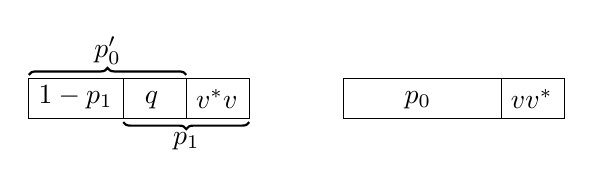
\begin{tikzpicture}
    \draw
            (0,0) rectangle (1.2,.5)
            (0,0) node[anchor=south west] {$1-p_1$}
            (1.2,0) rectangle (2,.5)
            (1.35,0) node[anchor=south west] {$q$} 
            (2,0) rectangle (2.8,.5)
            (2,0) node[anchor=south west] {$v^*v$} ;
    \draw [decorate,thick,decoration={brace}](2.8,-.05) -- (1.2,-.05) node[midway,anchor=north] {$p_1$};
    \draw [decorate,thick,decoration={brace}](0,.55) -- (2,.55) node[midway,anchor=south] {$p_0'$};
    \draw
            (4,0) rectangle (6,.5)
            (4.65,0) node[anchor=south west] {$p_0$} 
            (6,0) rectangle (6.8,.5)
            (6,0) node[anchor=south west] {$vv^*$} ;
\end{tikzpicture}
\end{center}
Note~$q = p_0'+p_1 - 1$ and~$p_0', p_1 \geq q$.
Define
\begin{equation*}
    D \ = \ \{d_0, d_1\} \qquad \text{where} \quad
    d_0 \ =\   e_1 q \qquad
    d_1 \ = \ e_0 + e_1v^*.
\end{equation*}
From~$p_1q=q$ it follows~$D$ is orthogonal.
Clearly~$\left<d_0,d_0\right>=q$ and
\begin{equation*}
    \left<d_1, d_1\right>
        \ =\ \left<e_0, e_0\right> + vp_1v^*    
        \ =\ p_0 + vv^* \ =\ 1.
\end{equation*}
So~$D$ is an orthonormal set.
Using~$0 = (1-p_0)p_0 = vv^*p_0 $ and~$q+v^*v = p_1$, we see
that for any~$x \equiv e_0 b_0 + e_1 b_1$
with~$b_0 \in p_0\scrB$ and~$b_1 \in p_1 \scrB$, we have
\begin{align*}
    d_0 \langle d_0, x \rangle + d_1 \langle d_1 , x \rangle
    &\ = \ d_0 b_1 + d_1(vb_1 + b_0) \\
    &\ = \ e_1 q b_1 + e_0 vb_1 + e_1v^*vb_1 + e_0 b_0 + e_1v^* b_0 \\
    &\ = \ e_1 q b_1 + e_0 p_0 vv^* vb_1 + e_1v^*vb_1 + e_0 b_0 + e_1v^* vv^* p_0 b_0 \\
    &\ = \ e_1 q b_1 + e_1v^*vb_1 + e_0 b_0  \\
    &\ = \ e_1 (q + v^*v) b_1 + e_0 b_0  \\
    &\ = \ e_1 b_1 + e_0 b_0 \ = \ x.
\end{align*}
Thus~$D$ is an orthonormal basis of~$\{e_0, e_1\}^{\perp\perp}$.
Hence~$E \equiv D \cup (E_1 - \{e_1\})$ is an orthonormal basis of~$X$
with~$d_1 \in E$ such that~$\left<d_1,d_1\right>=1$.
\end{point}
\begin{point}{70}%
For brevity, call~$X$ \Define{1-dim} if there is a one-element orthonormal basis of~$X$.
In~\sref{selfdual-normalish-form1} we saw
    how to create an orthonormal basis~$D$ of a non-1-dim~$X$
    with an~$e_0 \in D$ such that~$\left<e_0,e_0\right>=1$.
If~$\{e_0\}^\perp$ is not 1-dim,
    we can apply \sref{selfdual-normalish-form1}
    on~$\{e_0\}^\perp$ (instead of~$X$)
    to find an orthonormal basis~$D'$ of~$\{e_0\}^\perp$
    with~$e_1 \in D'$ such that~$\left<e_1,e_1\right>=1$.
This procedure can be continued using Zorn's lemma as follows.
Let~$P$ denote the poset of orthogonal subsets~$E \subseteq X$
    satisfying~$\langle e,e\rangle = 1$ for all~$e\in E$.
Clearly~$\emptyset\in P$
and for any non-empty chain~$C \subseteq P$
    we have~$\bigcup C \in P$.
By Zorn's lemma there is a maximal~$E \in P$.
Suppose~$E^\perp \neq \{0\}$ and~$E^\perp$ is not 1-dim.
Then by \sref{selfdual-normalish-form1}
    we can find an orthonormal basis~$E'$ of~$E^\perp$
    together with~$e \in E'$ such that~$\left<e,e\right>=1$.
Now~$E' \cup \{e\} \in P$, contradicting maximality of~$E$.
Apparently~$E^\perp = \{0\}$ or~$E^\perp$ is 1-dim.
If~$E^\perp = \{0\}$
    then we are done
    taking for~$\kappa$ the cardinality of~$E$.
For the other case, assume~$E^\perp = \{e\}^{\perp\perp}$
    for some~$e \in X$ with~$\left<e,e\right>$ a non-zero projection.
If~$E$ is finite, then we are done as well.
So, assume~$E$ is infinite.
Pick a sequence~$e_1, e_2, \ldots \in E$ of distinct elements.
Write~$p = \left<e,e\right>$
    and~$E_0 = \{e_n;\ n\in \N\}$.
Define
\begin{equation*}
    E_1 \ =\  \{e + e_1(1-p), \ e_1p + e_2(1-p),\  e_2p  +e_3(1-p),\  \ldots \}.
\end{equation*}
It is easy to see~$E_1$ is an orthogonal set
    with~$\left<d,d\right>=1$ for all~$d \in E_1$.
Furthermore~$E_1$ is an orthonormal basis for~$E_0 \cup \{e\}$,
    hence~$(E - E_0) \cup E_1$ is the desired orthonormal basis of~$X$. \qed
\end{point}
\end{point}
\end{point}
\begin{point}{80}%
Does this settle the issue raised
        in~\sref{thel2matter}?
      One might hope
    that~$\ell^2((1_{\mathscr{B}})_{\alpha \in \kappa}) \cong
        \ell^2((1_{\mathscr{B}})_{\beta\in\lambda})$
    implies~$\kappa=\lambda$ for all cardinals~$\kappa$,$\lambda$.
This is not the case.
Indeed, if~$\scrB$ is a type III factor
    of operators on a separable Hilbert space,
    then for any non-zero projection~$p$,
    we have~$p \sim 1 -p$ (by combining~\cite[dfn.~6.5.1]{kr}
        and~\cite[cor.~6.3.5]{kr})
    and so~$\scrB \cong p\scrB \oplus (1-p)\scrB \cong 
    \scrB \oplus \scrB$ as Hilbert C$^*$-modules.
\end{point}
\end{parsec}

\begin{parsec}{1630}%
\begin{point}{10}%
Before we continue to the next topic,
    the exterior tensor product of Hilbert C$^*$-modules,
    we will show that the ultranorm completion~\sref{dils-completion}
    is determined by its universal property.
    We will need this fact in our treatment
        of the exterior tensor product.
\end{point}
\begin{point}{20}[selfdual-compl-defining]{Proposition}%
Let~$\scrB$ be a von Neumann algebra and~$V$ a right~$\scrB$-module
    with~$\scrB$-valued inner product~$[\,\cdot\,,\,\cdot\,]$.
    \index{$[\,\cdot\,,\,\cdot\,]$!inner product!$\scrB$-valued}
There is an up-to-isomorphism unique
    self-dual Hilbert~$\scrB$-module~$X$
    together with inner product preserving $\scrB$-linear~$\eta \colon V \to X$
    with the following universal property.
    \begin{quote}
    For every bounded~$\scrB$-linear map~$T\colon V \to Y$
    to some self-dual Hilbert~$\scrB$-module~$Y$,
    there is a unique bounded~$\scrB$-linear map~$\hat{T}\colon X \to Y$
    with~$\hat{T} \after \eta = T$.
    \end{quote}
Moreover, for such~$\eta\colon V \to X$,
    the image of~$V$ under~$\eta$ is ultranorm dense.
\begin{point}{30}{Proof}%
We already know such a~$X$ and~$\eta\colon V \to X$
    exist by~\sref{dils-completion}
    and~\sref{selfdual-completion-univ}.
For this one~$\eta(V)$ is ultranorm dense in~$X$.
Assume there is another self-dual Hilbert~$\scrB$-module~$X_2$
    with inner product preserving~$\scrB$-linear~$\eta_2\colon V \to X_2$
    satisfying the universal property.
By the universal property of~$\eta$ applied to~$\eta_2$,
    there must exist a unique~$U \colon X  \to X_2$
    with~$U \after \eta  = \eta_2$.
Similarly, there is a~$V \colon X_2 \to X$
    with~$V \after \eta_2 = \eta$.
Clearly~$\id_{X} \after \eta = V \after \eta_2 = V \after U \after \eta$
    and so by the uniqueness~$\id = V\after U$.
    Similarly~$U \after V = \id$.
It remains to be shown~$U$ preserves the inner product.
As
\begin{equation*}
    \left<\eta(x),\eta(y)\right>
    \ =\  [x,y]
    \ =\  \left<\eta_2(x), \eta_2(y)\right>
    \ =\  \left<U \eta(x), U \eta(y)\right>
\end{equation*}
for all~$x,y \in X$, we know
$\eta(X)$ is ultranorm dense.
So by ultranorm continuity and bijectivity of~$U$,
    we know~$U(\eta(X)) = \eta_2(X)$ is ultranorm dense in~$X_2$.
Hence~$U$ preserves the inner product by~\sref{innerprod-ultraweak}
\qed
\end{point}
\end{point}
\end{parsec}

\subsection{Exterior tensor product}
\begin{parsec}{1640}%
\begin{point}{10}%
Suppose~$X$ is a Hilbert~$\scrA$-module
    and~$Y$ is a Hilbert~$\scrB$-module
    for some C$^*$-algebras~$\scrA$ and~$\scrB$.
The algebraic tensor product~$X \odot Y$
    is a right $\scrA \odot \scrB$-module
    via~$(x\otimes y)\cdot (a\otimes b) = (xa) \otimes (yb)$
    and has an~$\scrA \odot \scrB$-valued inner
    product fixed by~$[x\otimes y, x'\otimes y']
        = \left<x,x'\right> \otimes \left<y,y'\right>$.
Write~$\scrA \otimes_\sigma \scrB$ for the spatial
    C$^*$-tensor product~\cite[\S11.3]{kr} of~$\scrA$ and~$\scrB$.
The inner product on~$X \odot Y$ can be extended
    to an~$\scrA \otimes_\sigma \scrB$-valued inner product
    on the norm completion of~$X \odot Y$
    on which it is definite~\cite{lance}.
This is a Hilbert C$^*$-module,
    which is called the \emph{exterior tensor product} of~$X$ and~$Y$.
It is quite difficult to perform this construction:
    Lance discusses the difficulties in \cite[ch.~4]{lance}.
But if we assume~$\scrA$ and~$\scrB$ are von Neumann algebras
    \emph{and} that $X$ and~$Y$ are self-dual,
    it is rather easier.
In fact, we will directly construct the ultranorm completion
    of the exterior tensor product,
    which is a self-dual Hilbert $\scrA \otimes \scrB$-module,
    which we call the \emph{self-dual exterior tensor product}.
This self-dual exterior tensor product
    behaves much better than the plain exterior tensor product.
    As a first example, we will see (in \sref{ba-ext-tensor-pres})
    that~$\scrB^a(X) \otimes \scrB^a(Y) \cong \scrB^a(X\otimes Y)$
        for the self-dual exterior tensor product,
        which is false in general for the plain exterior tensor product.
The self-dual exterior tensor product also appears naturally
    when computing the Paschke dilation
    of a tensor product~$\varphi \otimes \psi$, see \sref{paschke-tensor}.
\end{point}
\begin{point}{20}[univprop-ext-tensor]{Theorem}%
Suppose~$\scrA$ and~$\scrB$ are von Neumann algebras.
For any self-dual Hilbert $\scrA$-module $X$
    and self-dual Hilbert~$\scrB$-module $Y$,
    there is an up-to-isomorphism unique
    self-dual Hilbert~$\scrA\otimes \scrB$-module
    $\Define{X \otimes Y}$, called the \Define{(self-dual exterior) tensor product}%
    \index{tensor product!of Hilbert $\scrB$-modules}%
    \index{*tensor@$\otimes$!Hilbert $\scrB$-modules},
    together with a~$\scrA \odot \scrB$-linear injective
    inner product preserving map~$\eta \colon X \odot Y \to X\otimes Y$
    with the following universal property.
    \begin{quote}
    For every self-dual~Hilbert~$\scrA\otimes\scrB$-module
    $Z$ with bounded~$\scrA \odot \scrB$-linear
        $T\colon X \odot Y \to Z$,
    there is a unique bounded~$\scrA \otimes \scrB$-linear
        map~$\hat{T}\colon X \otimes Y \to Z$
    with~$\hat{T} \after \eta= T$,
    \end{quote}
where we norm~$X \odot Y$ with~$\|t \| = \|[t,t]\|^{\frac{1}{2}}_{\scrA\otimes \scrB}$.
Write~$x \hotimes y = \eta(x\otimes y)$.
For any such~$X \otimes Y$ we have the following.
\begin{enumerate}
    \item The image of $X \odot Y$ under~$\eta$ is ultranorm dense in~$X \otimes Y$.
    \item If~$(e_i)_{i \in I}$ is an orthonormal basis of~$X$
                and~$(d_j)_{j \in J}$ of~$Y$,
                then
        \begin{enumerate}
            \item $(e_i \hotimes d_j)_{i,j\in I\times J}$
                is an orthonormal basis of~$X \otimes Y$ \emph{and}
            \item
                the linear span of
                \begin{equation*}
                    \{\, \ketbra{\,(e_i a) \hotimes (d_j b) \,}{\,
                        e_{k}\otimes d_{l} \,}; \ 
                        a \in \scrA, \ 
                        b \in \scrB,\ 
                        i,k \in I,\ 
                        j,l \in J \,
                    \} 
                \end{equation*}
                is ultraweakly dense in~$\scrB^a(X \otimes Y)$.
        \end{enumerate}
                
\end{enumerate}
\spacingfix{}
\begin{point}{30}{Proof}%
Pick orthonormal bases~$(e_i)_{i \in I}$ and~$(d_j)_{j \in J}$ of~$X$
    and~$Y$ respectively.
Write~$p_{ij} \equiv \left<e_i, e_i\right>\otimes \left<d_j,d_j\right>
    \in \scrA \otimes \scrB$.
Define~$X \otimes Y \equiv \ell^2((p_{ij})_{i,j \in I\times J})$,
    with~$\ell^2$ as in~\sref{hilbmod-el2}.
This definition of~$X \otimes Y$ seems to depend
    on the choice of bases~$(e_i)_i$ and~$(d_j)_h$.
    We show it does not (up-to-isomorphism), in \sref{ext-tensor-uniqueness}.
\begin{point}{40}[ext-tensor-dfn-eta]{Definition~$\eta$}%
Pick~$x \in X$ and~$y \in Y$.
Write~$x_i \equiv \left<e_i, x\right>$
and~$y_j \equiv \left<d_j, y\right>$.
Then
\begin{align*}
    \left<x,x\right> \otimes \left<y,y\right>
    &\ = \ \bigl( \sum_i x_i^*x_i\bigr) \otimes\bigl(\sum_jy_j^*y_j\bigr)
            &\quad&\text{by Parseval}  \\
            &\ = \ \sum_{i,j}  x_i^*x_i  \otimes y_j^*y_j \\
            &\ = \ \sum_{i,j}  (x_i \otimes y_j)^* (x_i  \otimes y_j).
\end{align*}
Hence~$(x_i \otimes y_j)_{i,j}$ is~$\ell^2$-summable,
    and so there is a unique~$\scrA \odot\scrB$-linear
    map~$\eta\colon X \odot Y \to X \otimes Y$ fixed
    by~$\eta(x \otimes y) = (x_i \otimes y_j)_{i,j}$.
\end{point}
\begin{point}{50}[ext-tensor-preserves-inner-prod]{$\eta$ preserves inner product}%
Pick additional~$x' \in X$ and~$y' \in Y$.
Writing~$x'_i = \left<e_i,x'\right>$
    and~$y'_j = \left<d_j, y'\right>$,
we have
\begin{equation*}
    \left<\eta(x\otimes y), \eta(x' \otimes y')\right>
    \ = \ \sum_{i,j} (x_i\otimes y_j)^* \otimes (x_i' \otimes y_j')
    \ = \ \sum_{i,j} x_i^*x_i' \otimes y_j^* y_j'
\end{equation*}
and
\begin{equation*}
    \bigl(\sum_i x_i^*x_i'\bigr) \otimes \bigl( \sum_j y_j^* y_j' \bigr)
    \ = \ \left<x,x'\right> \otimes \left<y,y'\right>
    \ = \ \left<x\otimes y,x' \otimes y'\right> .
\end{equation*}
Thus it is sufficient to show
    $\sum_{i,j} x_i^*x_i' \otimes y_j^* y_j'
    = \bigl(\sum_i x_i^*x_i'\bigr) \otimes \bigl( \sum_j y_j^* y_j' \bigr)$,
    which holds as the product np-functionals
    are separating by definition, see \sref{tensor}.
Thus indeed~$\eta$ preserves the inner product.
\end{point}
\begin{point}{60}{$\eta$ is injective}%
Let~$n \in \N$,~$x_1, \ldots, x_n \in X$
    and~$y_1,\ldots, y_n \in Y$
    be given such that~$\eta(\sum_l x_l \otimes y_l) = 0$
By~\sref{selfdual-gramschmidt}
    there are orthonormal~$e'_1,\ldots, e'_m \in X$
    such that~$x_l = \sum_i e'_i \langle e'_i, x_l\rangle$.
Similarly~$y_l = \sum_j d'_j \langle d'_j, y_l\rangle$
for some orthonormal~$d'_1, \ldots, d'_{m'} \in Y$.
As~$\eta$ preserves the inner product,
    the elements~$e_i'\hotimes d_j'$ are again orthonormal
    and so from
\begin{equation*}
    0 \ =\  \sum_l x_l \hotimes y_l
    \ =\  \sum_{i,j} (e'_i \hotimes d'_j) \bigl(\sum_l
         \langle e'_i, x_l\rangle \otimes \langle d'_j, y_l\rangle\bigr)
\end{equation*}
         it follows
         $\sum_l \langle e_i',x_l\rangle \otimes \langle d_j',y_l\rangle = 0$
         for all~$i,j$.
Consequently
\begin{equation*}
    \sum_l x_l \otimes y_l
        \ =\  \sum_{i,j} (e'_i \otimes d'_j) \bigl(\sum_l
        \langle e'_i, x_l \rangle \otimes \langle d'_j, y_l \rangle 
        \bigr) \ = \ 0,
\end{equation*}
which shows~$\eta$ is injective
    (and that the inner product on~$X \odot Y$ is definite).
\end{point}
\begin{point}{70}[ultranorm-dense-tensor-base]{Image $\eta$ ultranorm dense}%
For brevity, write~$E \equiv \{ e_i \hotimes d_j; \ i,j \in I\times J\}$.
By~\sref{tensor} (and \sref{ultraclosed})
    $\scrA \odot \scrB$ is ultrastrongly dense in~$\scrA \otimes \scrB$.
So~$E (\scrA \odot \scrB)$
    is ultranorm dense in~$E (\scrA \otimes \scrB)$,
    see~\sref{ultranormcontstruct}.
In turn the linear span of~$E (\scrA \otimes \scrB)$
    is (by construction) ultranorm dense in~$X \otimes Y$.
Thus the linear span of~$E (\scrA \odot \scrB)$
    is ultranorm dense in~$X \otimes Y$.
Hence the image of~$\eta$,
    which contains the linear span of~$E (\scrA \odot \scrB)$,
    is ultranorm dense in~$X \otimes Y$.
\end{point}
\begin{point}{80}{Universal property}%
Let~$Z$ be a self-dual~Hilbert $\scrA \otimes \scrB$-module
 with some bounded~$\scrA \odot \scrB$-linear $T\colon X \odot Y \to Z$.
If~$X \odot Y$ were an~$\scrA \otimes \scrB$-module
    \emph{and} both~$\eta$ and $T$ were~$\scrA \otimes \scrB$-linear,
    we could simply apply~\sref{selfdual-completion-univ}
    to get the desired~$\hat{T}$.
Instead, we will retrace the steps of its proof
    and modify it for the present situation.
Uniqueness of~$\hat{T}$ is the same:
    $\hat{T}$ is fixed by the ultranorm-dense image of~$\eta$
    as it is bounded~$\scrA\otimes\scrB$-linear
    and so ultranorm continuous by \sref{blinear-bounded-is-ultranorm}.
The argument for existence of~$\hat{T}$ is more subtle.
We will show
\begin{equation}\label{eq:exttensorcontT}
    \left<T t, T t\right> \leq \|T\|^2 [t,t]
        \qquad \text{for all~$t \in X \odot Y$}
\end{equation}
as a replacement for the ultranorm continuity of~$T$.
We cannot apply~\sref{blinear-inprod-inequality} directly:
    as~$\scrA \odot \scrB$ is not a C$^*$-algebra,
    we cannot construct~$(\left<t,t\right>+\varepsilon)^{-\frac{1}{2}}$
    required for its proof.
To prove \eqref{eq:exttensorcontT}, we will work in the norm completions.
Write~$\overline{\scrA \odot \scrB}$
    for the norm-closure of~$\scrA \odot \scrB$ in~$\scrA \otimes \scrB$.
Clearly~$\overline{\scrA \odot \scrB}$
    is a~C$^*$-algebra
    (in fact it is the spatial C$^*$-tensor product of~$\scrA$ and~$\scrB$).
Write~$\overline{X \odot Y}$
    for the norm-closure of the image of~$\eta$ in~$X \otimes Y$.
By norm continuity
    (see \sref{module-seminorm})
    the operations of~$X \otimes Y$
    restrict to turn~$\overline{X \odot Y}$ into a
    Hilbert~$\overline{\scrA \odot \scrB}$-module.
As~$T$ is uniformly continuous,
    there is a unique bounded~$\overline{\scrA\odot\scrB}$-linear
    $\overline{T}\colon \overline{X\odot Y} \to Z$
    with~$\overline{T} \after \eta = T$ and~$\|T\| = \|\overline{T}\|$.
Now we can apply the proof of~\sref{blinear-inprod-inequality}
    to~$\overline{T}$
    to find~$\langle \overline{T}s,\overline{T}s\rangle \leq
    \|\overline{T}\|^2\left<s,s\right>$
    for~$s \in \overline{X \odot Y}$.
Substituting~$s = \eta(t)$,
    we get \eqref{eq:exttensorcontT}.

To define~$\hat{T}$, pick any~$t \in X \otimes Y$.
As the image of~$\eta$ is ultranorm dense,
there is a net~$(\eta(t_\alpha))_\alpha$ with~$\eta(t_\alpha) \to t$ ultranorm.
For any~np-map~$f\colon \scrA\otimes \scrB \to \C$
\begin{align*}
    \|T(t_\alpha) - T(t_\beta) \|_f^2 
        &\ =\ f(\langle T(t_\alpha - t_\beta), T(t_\alpha - t_\beta) \rangle) \\
        & \ \leq \ \|T\|^2 f([t_\alpha-t_\beta, t_\alpha - t_\beta]) \\
        & \ = \ \|T\|^2 f(\left<\eta (t_\alpha)-\eta(t_\beta), \eta(t_\alpha) - \eta(t_\beta)\right>) \ \to\  0.
\end{align*}
So~$(T t_\alpha)_\alpha$ is ultranorm Cauchy in~$Z$.
With a similar argument we see~$(Tt_\alpha)_\alpha $
    is equivalent to~$ (T t'_\alpha)_\alpha$
whenever~$(\eta t_\alpha)_\alpha $ is equivalent
    to~$ (\eta t'_\alpha)_\alpha$.
So we may define
\begin{equation*}
\hat{T} t \ = \ \unlim_\alpha T t_\alpha.
\end{equation*}
Clearly~$\hat{T} \after \eta = T$.
With the same argument as for \sref{selfdual-completion-univ},
    we see~$\hat{T}$ is bounded and additive.
To show~$\hat{T}$ is~$\scrA\otimes \scrB$-linear,
    pick any~$b \in \scrA \otimes \scrB$.
There is a net~$b_\beta$ in~$\scrA \odot \scrB$
    with~$b_\beta \to b$ ultrastrongly.
If $\hat{T}$ is ultranorm continuous, we are done:
\begin{equation*}
    (\hat{T} t) b
    = \unlim_\beta (\unlim_\alpha T t_\alpha) b_\beta\\
     = \unlim_\beta \unlim_\alpha T (t_\alpha b_\beta) \\
     = \unlim_\beta \hat{T} (t b_\beta)\\
     = \hat{T} (tb).
\end{equation*}
To show~$\hat{T}$ is ultranorm continuous,
    assume~$t^\alpha \to 0$ ultranorm in~$X \otimes Y$.
It is sufficient to show~$\hat{T} t^\alpha \to 0$ ultranorm.
Let~$f\colon \scrA\otimes \scrB \to \C$ be any np-map.
Write~$\Phi$ for the set of entourages for ultranorm uniformity
    on~$X \otimes Y$.
As the image of~$\eta$ is ultranorm dense,
there is a~$\Phi$-indexed Cauchy net~$(t^\alpha_E)_{E \in \Phi}$ in
    $\eta (X \odot Y)$
    with~$t^\alpha_E \mathrel{E} t^\alpha$
    for each~$E \in \Phi$.
Thus~$\hat{T} t^\alpha = \unlim_E T t^\alpha_E$.
As~$t^\alpha \to 0$
    there is some~$\alpha_0$
    such that for all~$\alpha \geq \alpha_0$
    we have~$\|t^\alpha \|_f \leq \varepsilon$.
We can find~$E_0 \geq E_{f,\varepsilon}$
such that for all~$E \geq E_0$
we have~$\| \hat{T} t^{\alpha_0} -T t^{\alpha_0}_E \|_f \leq \varepsilon$.
For~$E \geq E_0$ we have~$E \geq E_{f,\varepsilon}$ and so
\begin{equation*}
 \|T t^{\alpha_0}_{E_0}\|_f
 \  \overset{\eqref{eq:exttensorcontT}}{\leq}\  \|T\| \|t^{\alpha_0}_{E_0}\|_f
  \  \leq\ \|T\|
  ( \|t^{\alpha_0}_{E_0} - t^{\alpha_0}\|_f +
  \| t^{\alpha_0} \|_f)
   \ \leq\  2 \|T\| \varepsilon.
\end{equation*}
    Consequently
\begin{equation*}
    \|\hat{T} t^{\alpha_0} \|_f \ \leq  \ 
    \|\hat{T} t^{\alpha_0} - T t^{\alpha_0}_{E_0} \|_f
                + \|T t^{\alpha_0}_{E_0}\|_f
    \ \leq\  \varepsilon + 2\|T\|\varepsilon.
\end{equation*}
So~$\hat{T}t^\alpha \to 0$ ultranorm, as desired.
\end{point}
\begin{point}{90}[ext-tensor-uniqueness]{Uniqueness}%
Assume there is a self-dual Hilbert~$\scrA\otimes\scrB$-module~$X \otimes_2 Y$
    together with a injective
    inner product-preserving~$\scrA\odot\scrB$-linear
    map~$\eta_2 \colon X \odot Y \to X \otimes_2 Y$
    also satisfying the universal property.
With the same reasoning as in \sref{selfdual-compl-defining}
    there is an invertible bounded~$\scrA\otimes\scrB$-linear
    $U\colon X \otimes Y \to X \otimes_2 Y$
    with~$U \after \eta = \eta_2$.
Clearly~$\left<Ux, U y\right> = \left<x,y\right>$
    for~$x,y \in E (\scrA\odot\scrB)$,
    where we defined~$E = \{e_i \hotimes d_j; \ i,j \in I\times J\}$.
As we saw the linear span of~$E (\scrA\odot\scrB)$
    is ultranorm dense in~$X \otimes Y$,
    we see~$U$ must preserve the inner product by \sref{innerprod-ultraweak}.
\end{point}
\begin{point}{100}%
Property 1 from the statement of the Theorem follows immediately
    from the fact that the exterior tensor product is unique
    up to an isomorphism which respects the embeddings.
Assume~$(e'_i)_{i \in I'}$ is an orthonormal basis of~$X$
    and~$(d'_j)_{j \in J'}$ is an orthonormal basis of~$Y$.
We will show $E_2 =\{ e'_i \hotimes d'_j; \ i,j \in I'\times J'\}$
is an orthonormal basis of~$X \hotimes Y$.
Clearly~$E_2$ is orthonormal.
By \sref{selfdual-orthn-basis} and \sref{hilbmod-projthm}
    it is sufficient to show~$e_{i_0} \hotimes d_{j_0} \in E_2^{\perp\perp}$
    for all~$i_0 \in I$ and $j_0 \in J$.
Write~$a_i = \left<e_i',e_{i_0}\right>$
    and~$b_j = \left<d_j',d_{j_0}\right>$.
By \sref{selfdual-orthn-basis} and \sref{ext-tensor-preserves-inner-prod}
    it suffices to show the latter equality in
    \begin{equation*}
        \bigl(\sum_i a_i^*a_i\bigr) \otimes \bigl(\sum_j b_j^*b_j\bigr) \ = \ 
    \langle e_{i_0}\hotimes d_{j_0}, e_{i_0}\hotimes d_{j_0}\rangle
    \ =\  \sum_{i,j} a_i^*a_i \otimes b_j^*b_j,
    \end{equation*}
    which holds as product np-functionals are separating
    by definition, see~\sref{tensor}.
\end{point}
\begin{point}{110}%
    Finally we prove that the linear span of
                \begin{equation*}
                    D \ \equiv \ \{ \ketbra{(e'_i a) \hotimes (d'_j b)}{
                        e_{k}\otimes d_{l} }; \ 
                        a \in \scrA, \ 
                        b \in \scrB,\ 
                        i,k \in I',\ 
                        j,l \in J'
                    \} 
                \end{equation*}
            is ultraweakly dense in~$\scrB^a(X \otimes Y)$.
By \sref{ketbra-ultraweakly-dense},
    the linear span
    of (the set of operators of
    the form)~$\ketbra{(e'_i \hotimes d'_j)t}{e'_k \hotimes d'_l}$
    with~$t \in \scrA \otimes \scrB$
    is ultraweakly dense in~$\scrB^a(X \otimes Y)$.
We will show that~$t \in \scrA \odot \scrB$ suffices.
    By~\sref{tensor}, \sref{ultraclosed} and~\sref{kaplansky},
    each~$t \in \scrA \otimes \scrB$
    is the ultrastrong limit
    of a norm bounded net~$t_\alpha$ in~$\scrA \odot \scrB$.
    So by \sref{ketbra-ultranorm-continuous} (and \sref{ultranormcontstruct}),
we see~$\ketbra{(e'_i \hotimes d'_j)t_\alpha}{e'_k \hotimes d'_l}$
converges ultraweakly to~$\ketbra{(e'_i \hotimes d'_j)t}{e'_k \hotimes d'_l}$.
So indeed, the linear span of~$D$
    is ultraweakly dense in~$\scrB^a(X \otimes Y)$. \qed
\end{point}
\end{point}
\end{point}

\begin{point}{120}{Examples}%
We give a few examples of the self-dual exterior tensor product
    and relate it to other notions of tensor product.
To avoid confusion, we will denote the self-dual exterior
    tensor product by~$\otimes_{\text{ext}}$
    (instead instead of the plain~$\otimes$.)
\begin{enumerate}
\item
Any Hilbert space is a self-dual Hilbert~$\C$ module.
For Hilbert spaces~$\scrH$ and~$\scrK$
    we have~$\scrH \otimes_{\text{Hilb}} \scrK
        \cong \scrH \otimes_{\text{ext}} \scrK$,
    where~$\otimes_{\text{Hilb}}$ denotes the regular tensor product of
    Hilbert spaces.
\item
Every von Neumann algebra is a self-dual Hilbert C$^*$-module
    over itself.
For any von Neumann algebras~$\scrA$ and~$\scrB$
    we have~$\scrA\otimes_{\text{vN}} \scrB
        \cong \scrA \otimes_{\text{ext}} \scrB$
        as Hilbert~$\scrA\otimes_{\text{vN}} \scrB$-modules,
        where~$\scrA\otimes_{\text{vN}}\scrB$ denotes the (spatial)
        tensor product of von Neumann algebras.
\item
Let~$X$ be a self-dual Hilbert~$\scrA$-module
    and~$Y$ be a self-dual Hilbert~$\scrB$-module
        for von Neumann algebras~$\scrA,\scrB$.
The norm closure of~$X\odot Y$
    in~$X \otimes_{\text{ext}} Y$
        is the plain exterior tensor product of~$X$ and~$Y$.
In turn, the ultranorm completion of the exterior tensor product
    of~$X$ and~$Y$ is isomorphic to~$X \otimes_{\text{ext}} Y$,
        the self-dual exterior tensor product.
\item
In~\sref{paschke-tensor} it will be shown that
\begin{equation*}
(\scrA_1 \otimes_{\varphi_1} \scrB_1)
    \otimes_{\text{ext}} (\scrA_2 \otimes_{\varphi_2} \scrB_2)
\ \cong \ 
(\scrA_1 \otimes \scrA_2) \otimes_{\varphi_1\otimes \varphi_2} (\scrB_1 \otimes \scrB_2)
\end{equation*}
        for all~ncp-maps $\varphi_i\colon \scrA_i \to \scrB_i$ ($i=1,2$)
    between von Neumann algebras.
\end{enumerate}
\spacingfix{}
\end{point}
\end{parsec}
\begin{parsec}{1650}%
\begin{point}{10}%
For Hilbert spaces~$\scrH$ and~$\scrK$,
    we have~$\scrB(\scrH \otimes \scrK)
        \cong \scrB(\scrH) \otimes \scrB(\scrK)$.
However, for Hilbert modules~$X$ and~$Y$
    and the regular (not necessarily self-dual)
        exterior tensor product
        it is not true in general
        that~$\scrB^a(X) \otimes \scrB^a(Y) \cong \scrB^a(X \otimes Y)$.
However, if~$X$ and~$Y$ are self-dual Hilbert modules over von Neumann
    algebras, then we do have the familiar formula
    for the self-dual exterior tensor product.
We need some preparation.
\end{point}
\begin{point}{20}{Setting}%
Let~$X$ be a self-dual Hilbert~$\scrA$-module
    and~$Y$ be a self-dual Hilbert~$\scrB$-module
    for von Neumann algebras~$\scrA$ and~$\scrB$.
\end{point}
\begin{point}{30}[dfn-tensor-of-hilbmod-maps]{Proposition}%
For any operators~$S \in \scrB^a(X)$ and~$T \in \scrB^a(Y)$,
there is a unique operator~$\Define{S \otimes T} \in \scrB^a(X\otimes Y)$%
    \index{*tensor@$\otimes$!module maps}%
    \index{tensor product!of module maps}
    fixed by~$(S \otimes T) (x \otimes y) = (S x) \otimes (T y)$
    for any~$x\in X$ and~$y \in Y$.
\begin{point}{40}{Proof}%
We will define~$S \otimes T$ using the universal
    property proven in \sref{univprop-ext-tensor}.
Write~$\Theta \colon X \odot Y \to X \otimes Y$
    for the map~$\Theta(x \otimes y) = (Sx) \otimes (Ty)$.
It is easy to see~$\Theta$ is~$\scrA \odot \scrB$-linear.
The hard part is to show that~$\Theta$ is bounded.
Pick any~$t \in X \odot Y$ --- say~$t \equiv \sum^n_{i=1} x_i \otimes y_i$.
To start, note~$(\left<Sx_i, Sx_j\right>)_{ij}$ is positive in $M_n \scrA$ ---
    indeed, for any~$a_1, \ldots, a_n \in \scrA$
    we have~$\sum_{i,j} a_i^* \left<S x_i, S x_j\right> a_j
            = \left<Sx,Sx\right> \geq 0$
                where~$x \equiv \sum_i x_i a_i$
                and so it is positive
                by \sref{when-a-matrix-over-a-cstar-algebra-is-positive}.
By reasoning in the same way for~$\sqrt{\|S\|^2 - S^*S}$
instead of~$S$,
it follows~$(\left<Sx_i, Sy_i \right>)_{ij} \leq (\|S\|^2 \left<x_i,x_j\right>)_{ij}$.
Similarly~$0 \leq (\left<Ty_i, Ty_j\right>)_{ij} \leq (\|T\|^2 \left<y_i, y_j\right>)_{ij}$ in~$M_n \scrB$.
Write~$s\colon (\scrA \otimes \scrB)^{\oplus n} \to \scrA \otimes \scrB$
    for the~$\scrA \otimes \scrB$-linear map
    given by~$s(t_1, \ldots, t_n) = t_1 + \cdots + t_n$.
    ($s$ is the \emph{row vector} filled with~$1$s).
It is easy to see~$s A s^* 1= \sum_{i,j} A_{ij}$
    for any matrix~$A$ over~$\scrA \otimes \scrB$.
As a final ingredient,
    recall that the
    bilinear map~$M_n(\otimes) \colon M_n \scrA \times M_n \scrB \to
                M_n( \scrA \otimes \scrB)$
        defined in the obvious way
        is positive by \sref{cp-bilinear} and \sref{tensor}.
    Putting everything together:
\begin{alignat*}{2}
    \langle \Theta t, \Theta t \rangle
        & \ = \ \sum_{i,j} \langle 
    (Sx_i) \otimes (Ty_i),
    (Sx_j) \otimes (Ty_j)
            \rangle  \\
        & \ = \ \sum_{i,j} 
    \langle Sx_i, S x_j \rangle
    \otimes \langle Ty_i, T y_j \rangle \\
    & \ = \ 
    s \,
    \left( 
    \langle Sx_i, S x_j \rangle
    \otimes \langle Ty_i, T y_j \rangle
\right)_{ij}  \,
     s^*1 \\
    & \ = \ 
     s \,
M_n(\otimes) \bigl(\,
    \left( 
    \langle Sx_i, S x_j \rangle \right)_{ij},
\left( \langle Ty_i, T y_j \rangle \right)_{ij} \,\bigr) 
\, s^*1 \\
    & \ \leq \ 
s \,
M_n(\otimes) \bigl(\,
    ( 
    \|S\|^2 \langle x_i,  x_j \rangle )_{ij},
(\|T\|^2 \langle y_i,  y_j \rangle )_{ij} \,\bigr) 
\, s^*1 \\
        & \ = \
    \|S\|^2\|T\|^2 \left<t,t\right>.
\end{alignat*}
We have proven that~$\Theta$ is bounded (by~$\|S\|\|T\|$).
Thus by \sref{univprop-ext-tensor},
    there exists a unique map~$S \otimes T \colon X\otimes Y \to X\otimes Y$
    with~$(S \otimes T) (x \otimes y) = \Theta(x \otimes y)
        \equiv (S x) \otimes (Ty)$,
        which is what we desired to prove. \qed
\end{point}
\end{point}
\begin{point}{50}[hilbmod-tensor-ketbra]{Exercise}%
Prove that for the
operation~$\otimes$ defined in \sref{dfn-tensor-of-hilbmod-maps}, we have
\begin{enumerate}
    \item $\ketbra{x_1}{x_2} \otimes \ketbra{y_1}{y_2}
            = \ketbra{x_1\otimes y_1}{x_2\otimes y_2}$,
        \item $1 \otimes 1 = 1$;
    \item $(S \otimes T) (S' \otimes T') = (SS' ) \otimes (TT')$
                \emph{and}
            \item $(S \otimes T)^* = S^* \otimes T^*$.

    (Hint:
    use that by the reasoning of \sref{ultranorm-dense-tensor-base}
    the linear
    span of
    \begin{equation*}
    \{ (e a) \otimes (d b); \ (a,b,e,d) \in \scrA \times \scrB
                    \times E \times D\}
    \end{equation*}
        is ultranorm dense in~$X \otimes Y$
        for any bases~$E$ of~$X$ and~$D$ of~$Y$.)

\end{enumerate}
\spacingfix{}
\end{point}
\begin{point}{60}[ba-ext-tensor-pres]{Theorem}%
There is an
    nmiu-isomorphism~$\vartheta\colon \scrB^a(X) \otimes \scrB^a(Y) \cong \scrB^a(X \otimes Y)$
    fixed by~$\vartheta(S\otimes T) = S \otimes T$.
\begin{point}{70}{Proof}%
We will show that
    the bilinear map~$\Theta \colon 
            \scrB^a(X) \times \scrB^a(Y) \to
    \scrB^a(X \otimes Y)$
    given by~$\Theta(S,T) = S \otimes T$
    is a tensor product in the sense of \sref{tensor}
    using~\sref{tensor-characterization}.
From this it follows
    by~\sref{tensor-uniqueness},
    that there is a
    nmiu-isomorphism
    \begin{equation*}
    \vartheta\colon \scrB^a(X) \otimes \scrB^a(Y) \ \cong\  \scrB^a(X \otimes Y)
    \end{equation*}
    with~$\vartheta(S\otimes T) = \Theta(S , T) = S \otimes T$, as promised.
\begin{point}{80}%
From \sref{hilbmod-tensor-ketbra}, it follows~$\Theta$ is an miu-bilinear map.
By~\sref{univprop-ext-tensor}
    the linear span of operators of the form~$
        \ketbra{e_i a}{e_k} \otimes \ketbra{d_j b }{d_l}
        = \ketbra{(e_i a) \otimes (d_j b)}{e_k \otimes d_l} $
        is ultraweakly dense in~$\scrB^a(X \otimes Y)$
        for an orthonormal basis~$e_i \otimes d_j$ of~$X \otimes Y$.
        So the image of~$\Theta$ generates~$\scrB^a(X\otimes Y)$.
\begin{point}{90}%
    It remains to be shown that there are sufficiently many product functionals
    (see~\sref{tensor} for the definition of product functional
    and their sufficiency).
    Write
    \begin{align*}
        \Omega_X &\ \equiv \ 
                    \{ f(\langle x, (\,\cdot\,) x \rangle);
                    \ f \colon \scrA \to \C \text{ np-map}, x\in X \} \\
        \Omega_Y& \  \equiv\ 
                    \{ g(\langle y, (\,\cdot\,) y \rangle);
                    \ g \colon \scrB \to \C \text{ np-map}, y\in Y \}.
    \end{align*}
From~\sref{hilbmod-ordersep}
    it follows~$\Omega_X$  and~$\Omega_Y$ are order separating.
For~$\sigma \in \Omega_X$ and~$\tau \in \Omega_Y$
 --- say~$\sigma \equiv f(\langle x, (\,\cdot\,) x\rangle)$,
    $\tau \equiv g(\langle y, (\,\cdot\,) y\rangle)$ ---
    define~$\sigma \otimes \tau \equiv
        (f \otimes g) (x \otimes y, (\,\cdot\,) x\otimes y) $
        and~$\Omega \equiv \{\sigma \otimes \tau; \sigma \in \Omega_X,
                    \ \tau \in \Omega_Y\}$.
We will show
    that~$\Omega$ is faithful
    and that~$(\sigma \otimes \tau)(\Theta(S,T)) = \sigma(S) \tau(T)$
    for all~$S \in \scrB^a(X)$ and~$T \in \scrB^a(Y)$,
    which is sufficient to show~$\Theta$ is a tensor product.
Indeed for any~$S \in \scrB^a(X)$ and $T \in \scrB^a(Y)$, we have
\begin{align*}
    (\sigma \otimes \tau)(\Theta(S, T))
        &\ = \ (f \otimes g) (\, \langle x \otimes y, 
                (S \otimes T) (x \otimes y) \rangle\,)\\
        &\ = \ (f \otimes g) (\,\langle x \otimes y, 
                (S x) \otimes (T y)\rangle\,)\\
        &\ = \ (f \otimes g) (\,
            \langle x, Sx\rangle \otimes
            \langle y, Ty\rangle \rangle\,)\\
        &\ = \ 
            f(\langle x, Sx\rangle ) \cdot
            g(\langle y, Ty\rangle \rangle)\\
        &\ = \ 
            \sigma(S) \tau(T).
\end{align*}
\end{point}
\spacingfix{}
\begin{point}{100}%
Finally, to show that~$\Omega$ is faithful,
        assume~$A \in \scrB^a(X \otimes Y)$, $A \geq 0$
        and $(\sigma \otimes \tau)(A) = 0$
        for all~$\sigma \otimes \tau \in \Omega$.
Then for all~$x \in X$ and~$y \in Y$,
    we have~$\langle x\otimes y, A (x\otimes y)\rangle = 0$,
        thus~$\| \sqrt{A} (x \otimes y) \|^2 = 0$,
        hence~$\sqrt{A} (x \otimes y) = 0$.
So~$\sqrt{A}$ vanishes on~$X \odot Y$,
    which is ultranorm dense in~$X \otimes Y$,
    whence~$\sqrt{A} = 0$. So~$A = 0$.
\qed
\end{point}
\end{point}
\end{point}
\end{point}
\end{parsec}

\begin{parsec}{1660}%
\begin{point}{10}%
To compute the tensor product of Paschke dilations,
    we will need to know a bit more about
    the ultranorm continuity of the exterior tensor product.
\end{point}
\begin{point}{20}[ultranorm-continuity-ext-tensor]{Lemma}%
Let~$X$ be a self-dual Hilbert~$\scrA$-module
    and~$Y$ be a self-dual Hilbert~$\scrB$-module
    for von Neumann algebras~$\scrA$ and~$\scrB$.
If~$x_\alpha \to x$ and~$y_\alpha \to y$ ultranorm
    for norm-bounded nets~$x_\alpha$ in~$X$ and~$y_\alpha$ in $Y$,
    then~$x_\alpha \otimes y_\alpha \to x \otimes y$ ultranorm.
\begin{point}{30}{Proof}%
As~$x_\alpha \otimes y_\alpha - x \otimes y
            = (x_\alpha -x )\otimes y_\alpha + x\otimes (y_\alpha - y)$,
            it is sufficient
    to show that both~$(x_\alpha -x) \otimes y_\alpha \to 0$
    and~$x\otimes (y_\alpha - y) \to 0$ ultranorm.
Clearly
\begin{align*}
    \langle (x_\alpha - x) \otimes y_\alpha,
        (x_\alpha - x) \otimes y_\alpha \rangle
    & \ = \ 
    \langle x_\alpha - x , x_\alpha - x \rangle\otimes 
    \langle y_\alpha ,y_\alpha \rangle \\
    & \ = \ 
    (\langle x_\alpha - x , x_\alpha - x \rangle\otimes 1) \cdot (1 \otimes 
    \langle y_\alpha ,y_\alpha \rangle ).
\end{align*}
The maps~$b \mapsto 1 \otimes b$ and~$a \mapsto a \otimes 1$
    are ncp % by \TODO{},
    so both~$1 \otimes \langle y_\alpha, y_\alpha \rangle$
    and~$\langle x_\alpha - x , x_\alpha - x \rangle\otimes 1$
    are bounded nets of positive elements.
    Also~$\langle x_\alpha - x , x_\alpha - x \rangle\otimes 1 \to 0$
        as~$x_\alpha \to x$ ultranorm.
Thus \sref{vanishing-effects} applies and we see
    $(\langle x_\alpha - x , x_\alpha - x \rangle\otimes 1) \cdot (1 \otimes 
    \langle y_\alpha ,y_\alpha \rangle ) \to 0$ ultraweakly,
    hence~$(x_\alpha - x) \otimes y_\alpha \to 0$ ultranorm.
With a similar argument
    one shows~$x\otimes (y_\alpha - y) \to 0$ ultranorm. \qed
\end{point}
\end{point}
\begin{point}{40}[exttensor-dense-subsets]{Lemma}%
Let~$X$ be a self-dual Hilbert~$\scrA$-module
    and~$Y$ be a self-dual Hilbert~$\scrB$-module
    for von Neumann algebras~$\scrA$ and~$\scrB$.
Suppose~$U \subseteq X$ and~$V \subseteq Y$
    are ultranorm-dense submodules.
Then the linear span of
\begin{equation*}
    U \otimes V \ \equiv\  \{ u \otimes v;\  u \in U,\ v \in V\}
\end{equation*}
is ultranorm dense in~$X \otimes Y$.
\begin{point}{50}{Proof}%
It is sufficient to show that every~$x \otimes y \in X \otimes Y$
    is the ultranorm limit of elements from~$U \otimes V$
    as the linear span of elements of the form~$x \otimes y$
    is ultranorm dense in~$X \otimes Y$.
So pick any element of the form~$x \otimes y \in X \otimes Y$.
By the Kaplansky density theorem for Hilbert C$^*$-modules,
 see \sref{kaplansky-hilbmod},
    there are norm-bounded nets~$x_\alpha$ in~$U$
    and~$y_\alpha$ in~$V$
    with~$x_\alpha \to x$ and~$y_\alpha \to y$ ultranorm.
So by \sref{ultranorm-continuity-ext-tensor},
    we see~$x_\alpha \otimes y_\alpha \to x \otimes y$. \qed
\end{point}
\end{point}
\begin{point}{60}[dilationspace-dense-subset]{Lemma}%
Let~$\varphi \colon \scrA \to \scrB$ be an ncp-map between von Neumann algebras
    together with ultrastrongly
    dense~$*$-subalgebras~$\scrA' \subseteq \scrA$
        and~$\scrB' \subseteq \scrB$.
Then: the linear span
    of~$ \scrT  \equiv \{ a \otimes b;\ a \in \scrA', \ b\in \scrB'\}$
is ultranorm dense in~$\scrA \otimes_\varphi \scrB$,
which was defined in  \sref{existence-paschke}.
\begin{point}{70}{Proof}%
It is sufficient to show that any~$a\otimes b \in \scrA \otimes_\varphi \scrB$
    is the ultranorm limit of elements from~$\scrT$.
    Pick any~$a\otimes b\in \scrA \otimes_\varphi \scrB$.
By \sref{dense-subalgebra}
    there are norm-bounded nets~$a_\alpha$ in~$\scrA'$ and
    $b_\alpha$ in~$\scrB'$
    with~$a_\alpha \to a$ and~$b_\alpha \to b$ ultrastrongly.
Say~$\|b_\alpha \|, \|a_\alpha\| \leq B$ for some~$B > 0$.
We will show~$a_\alpha \otimes b_\alpha - a\otimes b \to 0$ ultranorm.
As usual, we split it into two:
\begin{equation*}
a_\alpha \otimes b_\alpha - a \otimes b
\ = \ a_\alpha \otimes(b_\alpha -b )\  +\  (a_\alpha - a) \otimes b.
\end{equation*}
For the first term, note
\begin{align*}
    \langle a_\alpha \otimes (b_\alpha  - b),
    a_\alpha \otimes (b_\alpha  - b) \rangle
    & \ = \ 
    (b_\alpha - b)^* \,\varphi (a_\alpha^* a_\alpha) \,(b_\alpha - b) \\
    & \ \leq \ 
    B^2 \|\varphi\| \,(b_\alpha - b)^*  (b_\alpha - b),
\end{align*}
which converges to~$0$ ultraweakly as~$b_\alpha \to b$ ultrastrongly.
The second
\begin{align*}
    \langle
        (a_\alpha - a) \otimes b
        (a_\alpha - a) \otimes b \rangle
        & \ = \ 
        b^* \,\varphi((a_\alpha - a)^* (a_\alpha - a)) \, b,
\end{align*}
converges ultraweakly to~$0$
as and~$ b^* \varphi(\,\cdot\,) b$ is normal
and~$(a_\alpha - a)^*(a_\alpha - a)$ converges ultraweakly to~$0$
as~$a_\alpha \to a$ ultrastrongly. \qed
\end{point}
\end{point}
\end{parsec}

\begin{parsec}{1670}%
\begin{point}{10}[paschke-tensor]{Theorem}%
Suppose~$\varphi_i \colon \scrA_i \to \scrB_i$
    is an ncp-map between von Neumann algebras
    with Paschke dilation~$(\scrP_i, \varrho_i, h_i)$
    for~$i=1,2$.
Then~$(\scrP_1 \otimes \scrP_2, \varrho_1 \otimes \varrho_2, h_1\otimes h_2)$
    is a Paschke dilation of~$\varphi_1 \otimes \varphi_2$.
    Furthermore
\begin{equation}\label{tensor-of-paschke-dilation-spaces}
(\scrA_1 \otimes_{\varphi_1} \scrB_1)
\otimes (\scrA_2 \otimes_{\varphi_2} \scrB_2)
\ \cong \ 
(\scrA_1 \otimes \scrA_2) \otimes_{\varphi_1\otimes \varphi_2} (\scrB_1 \otimes \scrB_2).
\end{equation}
\spacingfix{}
\begin{point}{20}{Proof}%
We will prove \eqref{tensor-of-paschke-dilation-spaces} first.
We proceed as follows.
To start, we prove that~$
(\scrA_1 \odot \scrB_1) \odot (\scrA_2 \odot \scrB_2)$
    (with the obvious inclusion)
    is ultranorm dense in~$(\scrA_1 \otimes_{\varphi_1} \scrB_1)
\otimes (\scrA_2 \otimes_{\varphi_2} \scrB_2)$.
Then we show that~$
(\scrA_1 \odot \scrA_2) \odot (\scrB_1 \odot \scrB_2) $
is ultranorm dense in~$
(\scrA_1 \otimes \scrA_2) \otimes_{\varphi_1\otimes \varphi_2} (\scrB_1 \otimes \scrB_2)$.
We continue and show that the natural bijection
$U_0\colon (\scrA_1 \odot \scrB_1) \odot (\scrA_2 \odot \scrB_2) \cong
(\scrA_1 \odot \scrA_2) \odot (\scrB_1 \odot \scrB_2) $
preserves the induced inner products and
    so extends uniquely to an
    isomorphism~\eqref{tensor-of-paschke-dilation-spaces}.
Using this isomorphism,
    we prove that the tensor product of the standard Paschke dilations
    is a dilation of the tensor product.
    From this, we finally derive the stated result.
\begin{point}{30}[paschke-iso-tensor-density]{Density}%
By construction, $\scrA_1 \odot \scrB_1$ is an ultranorm-dense
        $\scrB_1$-submodule
    of~$\scrA_1 \otimes_{\varphi_1} \scrB_1$.
Similarly~$\scrA_2 \odot \scrB_2 $ is ultranorm dense
    in~$\scrA_2 \otimes_{\varphi_2} \scrB_2$.
Thus by \sref{exttensor-dense-subsets}
    $(\scrA_1 \odot \scrB_1) \odot(
    \scrA_2 \odot \scrB_2) $ is ultranorm dense in~$(\scrA_1 \otimes_{\varphi_1} \scrB_1)
\otimes (\scrA_2 \otimes_{\varphi_2} \scrB_2)$.
By \sref{tensor}
        (with~\sref{ultraclosed} and \sref{dense-subalgebra}),
    we know~$\scrA_1 \odot \scrA_2$
    is an ultrastrongly-dense subalgebra
    of~$\scrA_1 \otimes \scrA_2$.
Similarly~$\scrB_1 \odot \scrB_2$
    is ultrastrongly dense in~$\scrB_1 \otimes \scrB_2$.
Hence~$(\scrA_1 \odot \scrA_2) \odot 
    (\scrB_1 \odot \scrB_2)$ is ultranorm dense
    in
    $(\scrA_1 \otimes \scrA_2) \otimes_{\varphi_1 \otimes \varphi_2}
    (\scrB_1 \otimes \scrB_2)$
        by~\sref{dilationspace-dense-subset},
\end{point}
\begin{point}{40}{Inner product preservation}%
Clearly
\begin{alignat*}{2}
    &
    \bigl\langle\,
    (a_1 \otimes b_1)\otimes (a_2 \otimes b_2)\,,\,
    (\alpha_1 \otimes \beta_1 )\otimes( \alpha_2 \otimes \beta_2)
    \,\bigr\rangle \\
    & \qquad\ = \ 
    \langle a_1 \otimes b_1 , \alpha_1 \otimes \beta_1 \rangle \,\otimes\,
    \langle a_2 \otimes b_2 , \alpha_2 \otimes \beta_2 \rangle \\
    & \qquad\ = \ 
    (b_1^* \varphi_1( a_1^* \alpha_1) \beta_1)
    \,\otimes \,
    (b_2^* \varphi_2( a_2^* \alpha_2) \beta_2) \\
    & \qquad \ = \ 
    (b_1 \otimes b_2)^* \,(\varphi_1 \otimes \varphi_2)
    \bigl((a_1 \otimes a_2)^* (\alpha_1 \otimes \alpha_2)\bigr)
    \,(\beta_1 \otimes \beta_2) \\
    & \qquad \ = \ 
    \bigl\langle\,
    (a_1\otimes a_2)\otimes (b_1 \otimes b_2) \,,\,
    (\alpha_1\otimes \alpha_2)\otimes (\beta_1 \otimes \beta_2)
    \,\bigr\rangle;
\end{alignat*}
so $U_0 \colon (\scrA_1 \odot \scrB_1) \odot (\scrA_2 \odot \scrB_2) \cong
(\scrA_1 \odot \scrA_2) \odot (\scrB_1 \odot \scrB_2) $
preserves the inner product by linearity.
\end{point}
\begin{point}{50}%
As~$U_0$ preserves the inner product,
    it is ultranorm continuous.
So with the usual reasoning, there is a unique bounded
    $\scrB_1 \odot \scrB_2$-linear extension
\begin{equation*}
    U_1\colon (\scrA_1 \otimes_{\varphi_1} \scrB_1) \odot (\scrA_2 \otimes_{\varphi_2} \scrB_2) \ \to \ 
        (\scrA_1 \otimes \scrA_2) \otimes_{\varphi_1 \otimes \varphi_2} (\scrB_1 \otimes \scrB_2).
\end{equation*}
In turn, by the universal property of the self-dual exterior tensor product,
    there exists a unique
    bounded~$\scrB_1\otimes \scrB_2$-linear extension
\begin{equation*}
    U\colon (\scrA_1 \otimes_{\varphi_1} \scrB_1) \otimes (\scrA_2 \otimes_{\varphi_2} \scrB_2) \ \to\ 
        (\scrA_1 \otimes \scrA_2) \otimes_{\varphi_1 \otimes \varphi_2} (\scrB_1 \otimes \scrB_2).
\end{equation*}
    By the ultranorm density~\sref{paschke-iso-tensor-density}
    and \sref{innerprod-ultraweak}
    we know~$U$ also preserves the inner product.
    Also from~\sref{paschke-iso-tensor-density},
        it follows that~$U$ is surjective.
Thus~$U$ is an isomorphism with~$U^{-1} = U^*$.
    We have shown~\eqref{tensor-of-paschke-dilation-spaces}.
By \sref{ba-ext-tensor-pres}
there is a unique nmiu-isomorphism
\begin{equation*}
    \vartheta\colon
    \scrB^a (\scrA_1 \otimes_{\varphi_1} \scrB_1) \otimes
     \scrB^a(\scrA_2 \otimes_{\varphi_2} \scrB_2) \ \to\ 
    \scrB^a
     ((\scrA_1 \otimes_{\varphi_1} \scrB_1) \otimes
     (\scrA_2 \otimes_{\varphi_2} \scrB_2))
\end{equation*}
    fixed by~$\vartheta(S \otimes T) = S \otimes T$.
Let~$(\scrB^a((\scrA_1 \otimes \scrA_2) \otimes_{\varphi_1 \otimes \varphi_2} 
        (\scrB_1 \otimes \scrB_2)), \varrho, h)$
        and~$(\scrB^a(\scrA_i \otimes_{\varphi_i} \scrB_i), \varrho_i, h_i)$
    (for~$i=1,2$)
    denote the Paschke dilations
    of~$\varphi_1 \otimes \varphi_2$  and~$\varphi_i$, respectively,
    constructed in~\sref{existence-paschke}.
\end{point}%
\begin{point}{60}%
    Our next goal is to show
    \begin{align}\label{tensorpaschkesecondgoal}
    \ad_{U^*} \after \vartheta
                \after (\varrho_1 \otimes \varrho_2) &\ =\  \varrho
                & h \after \ad_{U^*} \after \vartheta 
                       & \ =\  h_1 \otimes h_2,
    \end{align}
    which is sufficient to show that~$(
        \scrB^a(\scrA_1 \otimes_{\varphi_1} \scrB_1)
        \otimes \scrB^a(\scrA_2 \otimes_{\varphi_2} \scrB_2),
        \varrho_1 \otimes \varrho_2,
        h_1 \otimes h_2)$
    is a Paschke dilation of~$\varphi_1 \otimes \varphi_2$.
    We start with the equation on the left.
\begin{align*}
    &\bigl((\ad_{U^*} \after \vartheta \after  (\varrho_1 \otimes \varrho_2)) (\alpha_1 \otimes \alpha_2)\bigr)
    \, (a_1 \otimes a_2) \otimes (b_1 \otimes b_2) \\
    &\qquad \ = \ 
    \bigl((\ad_{U^*} \after \vartheta) (\varrho_1 (\alpha_1)\otimes \varrho_2(\alpha_2)) \bigr)
    \, (a_1 \otimes a_2) \otimes (b_1 \otimes b_2) \\
    &\qquad \ = \ 
    U \,(\varrho_1 (\alpha_1)\otimes \varrho_2(\alpha_2)) \, U^*
    \, (a_1 \otimes a_2) \otimes (b_1 \otimes b_2) \\
    &\qquad \ = \ 
    U \,(\varrho_1 (\alpha_1)\otimes \varrho_2(\alpha_2)) 
    \, (a_1 \otimes b_1) \otimes (a_2 \otimes b_2) \\
    &\qquad \ = \ 
    U \,  ((\alpha_1 a_1) \otimes b_1) \otimes ((\alpha_2 a_2) \otimes b_2) \\
    &\qquad \ = \ 
     ((\alpha_1 \otimes \alpha_2)\cdot (a_1 \otimes a_2)) \otimes (b_1 \otimes b_2) \\
    &\qquad \ = \ 
    \varrho(\alpha_1 \otimes\alpha_2) \,(a_1 \otimes a_2) \otimes (b_1 \otimes b_2).
\end{align*}
As the linear span of
    elements of the form~$(a_1 \otimes a_2) \otimes (b_1 \otimes b_2)$
    is ultranorm dense in~$(\scrA_1 \otimes \scrA_2)
                            \otimes_{\varphi_1 \otimes \varphi_2}
                            (\scrB_1 \otimes \scrB_2) $,
    we see~$(\ad_{U^*} \after \vartheta \after (\varrho_1 \otimes \varrho_2))
            (\alpha_1 \otimes \alpha_2)
            = \varrho(\alpha_1 \otimes \alpha_2)$
            for all~$\alpha_1\in\scrA_1$ and~$\alpha_2\in\scrA_2$.
In turn, as the linear span of elements of the form~$\alpha_1 \otimes \alpha_2$
    is ultrastrongly dense in~$\scrA_1 \otimes \scrA_2$
    and ncp-maps are ultrastrongly continuous,
    we see~$\ad_{U^*} \after \vartheta \after (\varrho_1 \otimes \varrho_2) =
        \varrho$.
        We continue with the equation on the right
        of~\eqref{tensorpaschkesecondgoal}.
\begin{align*}
    (h \after \ad_{U^*} \after \vartheta) (T \otimes S)
        & \ = \ \langle (1 \otimes 1) \otimes (1 \otimes 1),
                        \ U\, (T \otimes S)\, U^*(1 \otimes 1) \otimes (1 \otimes 1)
                        \rangle \\
        & \ = \ \langle U^* \,(1 \otimes 1) \otimes (1 \otimes 1),
                        \  (T \otimes S)\, U^*(1 \otimes 1) \otimes (1 \otimes 1)
                        \rangle \\
        & \ = \ \langle (1 \otimes 1) \otimes (1 \otimes 1),
                        \  (T \otimes S)\, (1 \otimes 1) \otimes (1 \otimes 1)
                        \rangle \\
        & \ = \
        \langle 1 \otimes 1, \,T\, 1\otimes 1\rangle \,\otimes\,
        \langle 1 \otimes 1, \,S\, 1\otimes 1\rangle \\
        & \ = \
        h_1(T) \otimes h_2(S) \\
        & \ = \
        (h_1\otimes h_2)(T \otimes S)
\end{align*}
From ultrastrong density, again, it
    follows~$h \after \ad_{U^*} \after \vartheta = h_1 \otimes h_2$. \qed
\end{point}
% \begin{point}%
% Assume that~$(\scrP_i, \varrho_i', h_i')$
%     is any (other) Paschke dilation of~$\varphi_i$ (for~$i=1,2$).
% Then there are isomorphisms~$\beta_1,\beta_2$
%     with~$\beta_i \after \varrho_i = \varrho_i'$
%     and~$h_i' \after \beta_i = h_i$.
% So~$\varrho'_1 \otimes \varrho'_2
%         = (\beta_1 \otimes \beta_2) \after (\varrho_1 \otimes \varrho_2)$
%         and~$(h_1' \otimes h_2') \after (\beta_1 \otimes \beta_2) = h_1 \otimes h_2$.
% As~$\beta_1 \otimes \beta_2$ is an isomorphism,
%     the previous shows that~$(\scrP_1 \otimes \scrP_2, \varrho_1' \otimes \varrho_2', h_1' \otimes h_2')$ is also a Paschke dilation of~$\varphi_1 \otimes \varphi_2$. \qed
% \end{point}
\end{point}
\end{point}
\end{parsec}

\section{Pure maps}
\begin{parsec}{1680}%
\begin{point}{10}%
Schr\"odinger's equation is invariant under the reversal of time
    and so the isolated quantum mechanical processes (ncp-maps) described by
    it are invertible.
In stark contrast, the ncp-maps corresponding to measurement and discarding
    are rarely invertible.
There are, however, many  processes in between
    which might not be invertible, but are still pure enough to be `reversed'
        in some consistent and useful fashion.
For instance, the ncp-map~$\ad_V$
    has the obvious reversal~$(\ad_V)^\dagger = \ad_{V^*}$
        (which is in general not the inverse.)
    Stinespring's theorem (\sref{stinespring-theorem})
        implies that every ncp-map into~$\scrB(\scrH)$
    splits as a reversible~$\ad_V$ after a (possibly) non-reversible
    nmiu-map~$\varrho$.
Using Paschke's dilation,
    we see that every ncp-map factors
    as an nmiu-map~$\varrho$ before some particular~ncp-map~$h$.
Is this~ncp-map~$h$ reversible in some sense?
In~\sref{paschke-pure} we will see that these~$h$
    are pure (in the sense of \sref{pure})
    and in~\sref{dagger-theorem}
    we will see that these pure maps are (in a sense) reversible.
\begin{point}{20}%
The reversibility of pure maps (in a much more general setting)
    is the main result of the next chapter.
In the remainder of this chapter, we study purity of ncp-maps a bit more.
We consider a seemingly unrelated  alternative notion of purity,
    which is based on Paschke's dilation,
    and show (in \sref{paschke-pure})
    that this alternative notion is in fact equivalent to the original.
We end this chapter by giving a different proof
    of the ncp-extremeness of pure and nmiu-maps.
\end{point}
\begin{point}{30}[dils-pure-discussion]%
Before we continue, let's rule out generalizations
    of more familiar notions of purity
    to arbitrary ncp-maps.
\begin{enumerate}
\item
A state~$\varphi\colon \scrA \to \C$ is called pure if it is an extreme
    point among all states.
It is unreasonable to define an arbitrary ncp-map to be pure
    if it is extreme, as every nmiu-map (including 
    von Neumann measurements and discarding)
    is extreme among the unital ncp-maps.
This follows from~\sref{rigid-ncp-extreme} and~\sref{nmiu-rigid},
    but will be proven again in~\sref{nmiu-ncp-extreme}.
In fact, in \sref{ncp-extreme-comp}
    we show that every ncp-map is the composition
    of two extreme maps.

\item
Inspired by the GNS-correspondence between pure states and
    irreducible representations,
St\o rmer defines a map~$\varphi\colon \scrA \to \scrB(\scrH)$ to be pure
    if the only maps below~$\varphi$ in the completely positive ordering
    are scalar multiples of~$\varphi$.
For every central element~$z$ of~$\scrA$,
    the map~$a \mapsto za$ is below~$\id_\scrA$
    and so the identity on non-factors is not pure in the sense
        of St\o rmer,
        even though the identity map is clearly reversible.
\end{enumerate}
\spacingfix{}
\end{point}
\begin{point}{40}%
Let's recall how we came to the notion of purity in \sref{pure},
    by generalizing~$\ad_V$.
Pick~$V \colon \scrH \to \scrK$.
    By polar decomposition, see~\sref{polar-decomposition}, we know that~$V = U A$
    for~$A \equiv \sqrt{V^*V} \colon \scrH \to \ceil{A} \scrH$
    and some isometry~$U \colon \ceil{A} \scrH \to \scrK$.
Thus we have~$\ad_V = \ad_A \after \ad_U$.
These two maps admit dual universal properties:
    $\ad_U$ is a \emph{corner}
    and~$\ad_A$ is a \emph{filter}.
An ncp-map~$\varphi$ is pure
    if it is the composition of a filter after a corner.
It turns out that~$\varphi$ is pure in this sense
    if and only if the map on the left-hand side of
    its Paschke dilation is surjective.
\end{point}
\end{point}
\end{parsec}

\begin{parsec}{1690}%
\begin{point}{10}%
We recall the definition of corner
        from \cite[dfn.~2]{westerbaan2016universal} and \sref{corner}.
\end{point}
\begin{point}{20}[dils-corner]{Definition}%
An ncp-map~$h \colon \scrA \to \scrB$
is a \Define{corner}\index{corner} for~$a \in [0,1]_\scrA$ if~$h(a)=h(1)$
    and
    \begin{quote}
        for every ncp-map $f\colon \scrA \to \scrC$
            with~$f(1)=f(a)$,
            there is a unique ncp-map~$f'\colon \scrB \to \scrC$
            with~$f = f' \after h$.
    \end{quote}
\spacingfix{}
\begin{point}{30}{Remark}%
In the next chapter we will study maps with a similar universal property
    as corners in a more general setting,
    but with all arrows in the reverse direction.
To help alleviate some confusion caused by the change of direction,
    we call those maps \emph{comprehensions},
    see \sref{dfn-comprehension}.  See also~\cite{effintro}.
\end{point}
\end{point}
\begin{point}{40}{Example}%
    The map~$h_a \colon \scrA \to \floor{a} \scrA \floor{a}$ given
    by~$b \mapsto \floor{a} b \floor{a}$
    is a corner of~$a \in [0,1]_\scrA$.
    We call~$h_a$ the \Define{standard corner}\index{corner!standard} of~$a$.
    See \sref{dfn-standard-corner-and-filter}, \sref{prop-corner}
        or \cite[prop.~5]{westerbaan2016universal}.
\end{point}
\begin{point}{50}[h-is-corner-for-unital-map]{Lemma}%
If~$(\scrP, \varrho, h)$ is a Paschke dilation of a unital ncp-map,
    then~$h$ is a corner.
\begin{point}{60}{Proof}%
(This is a different proof of our similar result \cite[cor.~27]{wwpaschke}.)
Let~$\varphi \colon \scrA \to \scrB$ be any unital ncp-map.
It is sufficient to prove~$h$
    is a corner for the
    standard dilation~$(\scrP , \varrho, h)$
    constructed in \sref{existence-paschke},
    so~$\scrP \equiv \scrB^a(\scrA \otimes_\varphi \scrB)$
    and~$h(T) = \langle e, T e\rangle$, where~$e \equiv 1\otimes 1$.
    Write~$p \equiv \ketbra{e}{e}$.
From~$\langle e,e\rangle = \varphi(1) = 1$
    it follows~$p$ is a projection.
Define~$\vartheta\colon \scrB \to p \scrP p$
    by~$\vartheta(b) = \ketbra{e \cdot b}{e}$.
    Some straightforward computations (using~\sref{hilbmodketbrarules})
    show~$\vartheta$ is an miu-map
    with inverse~$pTp \mapsto h(pTp)$.
So~$\vartheta$ is an miu-isomorphism and thus also normal.
    Furthermore~$h = \vartheta^{-1}(p (\,\cdot\,) p)$
     and so~$h$ is indeed a corner (of~$p$). \qed
\end{point}
\end{point}
\begin{point}{70}%
We recall the definition of filter, see \sref{filter}. 
\end{point}
\begin{point}{80}[dils-def-filter]{Definition}%
An ncp-map~$c \colon \scrA \to \scrB$
is a \Define{filter}\index{filter} for~$b \in\scrB$, $b \geq 0$ if~$c(1)\leq b$
    and
    \begin{quote}
        for every ncp-map $f\colon \scrC \to \scrB$
            with~$f(1) \leq b$,
            there is a unique ncp-map~$f'\colon \scrC \to \scrA$
            with~$f = c \after f'$.
    \end{quote}
\spacingfix{}
\begin{point}{90}{Remark}%
The direction-reversed counterpart
    of filters are called \emph{quotients},
    see~\sref{dfn-quotient} and~\cite{effintro} .
Filters were introduced by us in \cite[dfn.~2]{westerbaan2016universal}
    under the name \emph{compressions}.
To avoid confusion with \cite{alfsen2012}
    and be closer to e.g.~\cite{wilce2016royal},
    we changed the name from compression to filter.
Filters are named after polarization filters:
    the action of a polarization filter on the polarization
        of a photon is the same as a filter for
        the projection of the space of polarizations
        the polarization filter allows to pass without disturbance.
Combining two polarization filters corresponds
    to composing the corresponding filters.
This composed filter is in general a filter for an effect instead
    of a projection.
This corresponds with the fact that there might not be a polarization
    of the photon anymore,
    with which it can pass both filters undisturbed.
\end{point}
\end{point}
\begin{point}{100}[dils-stand-filter]{Example}%
    The map~$c_b\colon \scrB \to \ceil{b} \scrB \ceil{b}$
        given by~$a \mapsto \sqrt{b} a \sqrt{b}$ is a filter
        of~$b\in \scrB$, $b\geq 0$.
        We call~$c_b$ the \Define{standard filter}\index{filter!standard} of~$b$.
    See \sref{canonical-filter}, \sref{dfn-standard-corner-and-filter}
        or \cite[prop.~6]{westerbaan2016universal}.
\end{point}
\begin{point}{110}[dils-filter-basics-exercise]{Exercise}%
Let~$\varphi\colon \scrA \to \scrB$ be any ncp-map
    between von Neumann algebras.
\begin{enumerate}
\item
    Let~$c \colon \scrB \to \scrC$ be any filter.
    Show that if~$(\scrP, \varrho, h)$ is a Paschke dilation
            of~$\varphi$,
    that then~$(\scrP, \varrho, c \after h)$ is a Paschke dilation
        of~$c \after \varphi$.
\item
    Assume~$c'\colon \scrC' \to \scrB$ is a filter of~$\varphi(1)$.
    Prove that there is a unique unital ncp-map~$\varphi'$
        with~$\varphi = c \after \varphi'$.
    Conclude that if~$(\scrP, \varrho, h)$ is a Paschke dilation
            of~$\varphi'$,
            that then~$(\scrP, \varrho, c' \after h)$
            is a Paschke dilation of~$\varphi$.
\end{enumerate}
(See \sref{dils-abstract-basics} and \sref{quotient-total} for the proofs
        in the more general case.)
\end{point}
\begin{point}{120}[dils-filters-injective]{Exercise}%
Derive (perhaps from~\sref{dils-stand-filter} and~\sref{mult-cancellation}),
    that filters are injective.
\end{point}
\end{parsec}
\begin{parsec}{1700}%
\begin{point}{10}[dils-def-pure]{Definition}%
    Filters, corners and their compositions are called \Define{pure}.
    \index{pure!ncp-map}
\begin{point}{11}{Remark}%
This definition is equivalent to our previous definition
    of purity given in \cite[dfn.~21]{wwpaschke};
    see~\sref{pure-fundamental}.
\end{point}
\end{point}
\begin{point}{20}[dils-examples-pure]{Examples}%
Isomorphisms are pure.  Less trivial examples follow.
\begin{enumerate}
\item
The pure maps~$\scrB(\scrH) \to \scrB(\scrK)$
    are precisely of the form~$\ad_T$
    for some bounded operator~$T\colon \scrK \to \scrH$.
\item
Let~$(\scrP, \varrho, h)$ be a Paschke dilation of some ncp-map~$\varphi$.
In \sref{h-is-corner-for-unital-map} we saw that if~$\varphi$ is unital,
        that then~$h$ is a corner (and thus pure).
In general, $h = c \after h'$ for some filter~$c$ and corner~$h'$
    by \sref{dils-filter-basics-exercise},
        and so~$h$ is pure.
\end{enumerate}
\spacingfix{}
\end{point}
\begin{point}{30}{Remark}%
By definition, the set of pure maps is closed under composition.
In the next chapter we will see (\sref{dagger-theorem}) that
    there is a unique dagger~$\dagger$
    which turns the subcategory of von Neumann
    algebras with pure maps into a~$\dagger$-category
    such that~$f^\dagger$ is contraposed to~$f$;
            $\diamond$-positive maps are~$\dagger$-positive
            and~$\dagger$-positive maps have unique roots.
For this unique~$\dagger$, we have~$(\ad_V)^\dagger = \ad_{V^*}$.
\end{point}
\begin{point}{40}[surjective-nmiu]{Exercise}%
Show that any surjective nmiu-map between von Neumann algebras
        is a corner of a central projection, hence pure
        --- and conversely,
        that any corner of a central projection is a surjective nmiu-map.
\end{point}
\end{parsec}

\begin{parsec}{1710}%
\begin{point}{10}%
We will prove that a map is pure if and only if
    the left-hand side map of its Paschke dilation
    is surjective.  We need the following result.
\end{point}
\begin{point}{20}[paschke-corner]{Theorem}%
Let~$\scrA$ be a von Neumann algebra together with a projection~$p \in \scrA$.
Then a Paschke dilation of the standard corner~$h_p \colon \scrA \to p\scrA p$,
$a \mapsto pap$
is given by~$(\cceil{p}\scrA, h_{\cceil{p}}, h'_p)$,
    where~$\cceil{p}$ is the central  carrier of~$p$,
    see \sref{cceil-fundamental};
    $h_{\cceil{p}}$ is the standard corner for~$\cceil{p}$
        and~$h'_p \colon \cceil{p} \scrA \to p\scrA p$
        is the restriction of~$h_p$.
\begin{point}{30}{Proof}%
(This is a simplified proof of the result we published earlier.
    \cite[thm.~28]{wwpaschke})
Let~$(\scrA \otimes_{h_p} p\scrA p, \varrho, h)$
    denote the Paschke dilation constructed in~\sref{existence-paschke}.
We proceed in three steps:
    first we show~$\scrA p$ is a self-dual Hilbert~$p\scrA p$-module,
    then we prove~$\scrA \otimes_{h_p} p\scrA p \cong \scrA p$
    and finally we show~$\scrB^a(\scrA p) \cong \cceil{p} \scrA$.
\begin{point}{40}%
Note $\scrA p$ is a pre-Hilbert $p \scrA p$-module
    with scalar multiplication~$(\alpha p)\cdot (pap) = \alpha pap$
    and inner product~$\left<\alpha p, ap\right> = p\alpha^*ap$.
Since by the C$^*$-identity the norm on~$\scrA p$
    as a Hilbert module coincides with that as a subset of~$p \scrA p$;
    $\scrA p$ is norm closed in~$\scrA$ \emph{and}~$\scrA$ is norm complete,
    we see~$\scrA p$ is a Hilbert~$p \scrA p$-module.

Recall~$\scrA$ itself is a self-dual Hilbert~$\scrA$-module.
The uniformity induced on~$\scrA p$ by the ultranorm uniformity
    of~$\scrA$ coincides with the ultranorm uniformity of~$\scrA p$ itself.
The module $\scrA p$ is ultranorm closed in~$\scrA$
    as~$x_\alpha \to x$ ultranorm
    implies~$x_\alpha p \to xp$ ultranorm.
As self-duality is equivalent to ultranorm completeness,
    we see~$\scrA p$ is self dual as well.
\end{point}
\begin{point}{50}%
Concerning~$\scrA \otimes_{h_p} p \scrA p \cong \scrA p$,
    define~$B\colon \scrA \times  p \scrA p \to \scrA p$
    by~$B(\alpha, pap) = \alpha pap$.
A straightforward computation
    shows~$B$ is a~$h_p$-compatible complex bilinear map
    (see \sref{phi-compatible-paschke})
    and so by \sref{existence-paschke},  there is a unique bounded module
    map~$U \colon \scrA \otimes_{h_p} p \scrA p \to \scrA p$
    fixed by~$U (\alpha \otimes pap) = B(\alpha,pap) \equiv \alpha pap $.
We will show~$U$ is an isomorphism.
   Clearly~$U$ is surjective.

An easy computation shows~$a \otimes p\alpha p - ap\alpha p \otimes p = 0$
    for all~$a, \alpha \in \scrA$.
So the set~$\{a \otimes p;\ a\in \scrA\}$
    is ultranorm dense in~$\scrA \otimes_{h_p} p \scrA p$.
From this and
    $\left<\alpha \otimes p, a\otimes p\right> = 
        p \alpha^* a p
        =\left< U \alpha \otimes p, U a \otimes p\right> $
        we see~$U$ preserves the inner product.
Hence~$U$ is an isomorphism with~$U^* = U^{-1}$
    given by~$U^* a = a\otimes p$.
\end{point}
\begin{point}{60}%
To show~$\scrB^a(\scrA p) \cong \cceil{p}\scrA$,
we will first find a convenient orthonormal basis of~$\scrA p$.
By \sref{cceil-sum},
    there are partial isometries~$(u_i)_i$
    with~$\sum_i u_iu_i^* = \cceil{p}$
    and~$u_i^*u_i \leq p$.
Write~$E = \{u_i; \ i \in I\}$.
As~$u_i = u_i p$ and~$u_i= u_i u_i^* u_i$
    we see~$E$ is an orthonormal subset of~$\scrA p$.
For any~$ap \in \scrA p$, we have
\begin{equation*}
    ap \ =\  a \cceil{p} p
       \ =\  \cceil{p} a p
       \ = \ \bigl(\sum_i u_i u_i^*\bigr) ap
       \ = \ \sum_i u_i u_i^* ap
       \ = \ \sum_i u_i \left<u_i,ap\right>,
\end{equation*}
where the sums converge ultrastrongly in~$\scrA$.
Thus the last sum converges ultranorm in~$\scrA p$ as well.
Hence~$E$ is an orthonormal basis of~$\scrA p$.

Define~$\varrho_0 \colon \scrA \to \scrB^a(\scrA p)$
    by~$\varrho_0 = \ad_{U^*} \after \varrho$.
Note~$\varrho_0$ is an nmiu-map and~$\varrho_0(\alpha)ap = \alpha ap$.
The map~$\varrho_0$ is surjective:
    indeed for any~$T \in \scrB^a(\scrA p)$
\begin{equation*}
    T (ap) \ = \ \sum_i T( u_i ) u_i^* ap
           \ = \ \bigl(\sum_i T( u_i ) u_i^*\bigr) ap
           \ = \ \varrho_0 \bigl(\sum_i T( u_i ) u_i^*\bigr) ap.
\end{equation*}
Next, we show~$\ceil{\varrho_0} = \cceil{p}$.
It suffices to prove for all~$\alpha \in \scrA$,$\alpha \geq 0$, that
\begin{equation*}
    \alpha ap = 0 \text{ \ for all\  } a\in \scrA
    \quad\iff \quad
    \alpha \cceil{p} = 0.
\end{equation*}
    Clearly,
    $\alpha \cceil{p} = 0$ implies~$\alpha ap = \alpha \cceil{p} ap= 0$.
For the converse, assume that we have~$\alpha ap = 0$ for all~$a\in\scrA$.
Then in particular~$\alpha u_ip = 0$,
    hence~$\alpha \cceil{p} = \alpha \sum_i u_iu_i^*  = \sum_i \alpha u_ipu_i^*=0$.
    Indeed~$\ceil{\varrho_0} = \cceil{p}$.

    By~\sref{surjective-nmiu}
    there is an nmiu-isomorphism~$\varphi\colon
    \cceil{p} \scrA \to \scrB^a(\scrA p)$
    with~$\varrho_0 = \varphi \after h_{\cceil{p}}$.
Hence~$h_{\cceil{p}} = (\varphi^{-1} \after \ad_{U^*}) \after \varrho$.
We compute
\begin{equation*}
h'_p \after h_{\cceil{p}}
    \ = \ h_p
    \ =\  h \after \varrho
    \ =\ h \after \ad_U \after \varrho_0
    \ = \ h \after \ad_U \after \varphi \after h_{\cceil{p}}.
\end{equation*}
Using surjectivity of~$h_{\cceil{p}}$
and rearranging, we find~$h'_p \after (\varphi^{-1} \after \ad_{U^*}) = h$.
Thus indeed~$(\cceil{p} \scrA, h_{\cceil{p}}, h'_p)$
is a Paschke dilation of~$h_p$.  \qed
\end{point}
\end{point}
\end{point}
\begin{point}{70}[paschke-pure]{Theorem}%
    Let~$\varphi\colon \scrA \to \scrB$ be an ncp-map
    between von Neumann algebras with
    Paschke dilation~$(\scrP, \varrho, h)$.
The map~$\varphi$ is pure if and only if~$\varrho$ is surjective.
\begin{point}{80}{Proof}%
Assume~$\varrho$ is surjective.
The kernel of~$\varrho$ is an ultraweakly closed
two-sided ideal and so~$\ker\varrho = z \scrA$ for some central projection~$z$,
see \sref{prop:weakly-closed-ideal}.
The standard corner~$h_{z^\perp} \colon \scrA \to z^\perp \scrA$
    is the quotient-map of~$z \scrA$
    and so by the isomorphism theorem $\varrho$ is a corner as well.
In \sref{dils-examples-pure} we saw~$h$ is pure.
So~$\varphi$ is the composition of pure maps, hence pure itself.

For the converse, assume~$\varphi$ is pure.
For brevity, write~$p \equiv \ceil{\varphi}$.
There is a unique ncp-map~$c$ with~$\varphi = c \after h_p$,
    where~$h_{\ceil{\varphi}}$ is the standard corner of~$p$.
The map~$c$ is a filter,
    see \sref{square-f}.
By \sref{paschke-corner},
    the triple~$(\cceil{p}\scrA, h_{\cceil{p}}, h'_p)$
    is a Paschke dilation of~$h_p$,
    where~$h'_p$ denotes the restriction of~$h_p$ to~$\cceil{p} \scrA$.
So by \sref{dils-filter-basics-exercise}
    we see~$(\cceil{p}\scrA, h_{\cceil{p}}, c\after h'_p)$
    is a Paschke dilation of~$ \varphi$.
Clearly~$h_{\cceil{p}}$ is surjective.
If~$(\scrP', \varrho', h')$ is any other Paschke dilation of~$\varphi$,
    then~$\varrho' = \vartheta \after h_{\cceil{p}}$
    for some isomorphism~$\vartheta$
    and so~$\varrho'$ is surjective as well. \qed
\end{point}
\end{point}
\end{parsec}

\begin{parsec}{1720}[paschke-corresp-pure]%
\begin{point}{10}%
The order correspondence \sref{paschke-correspondence}
    has several corollaries.
\end{point}
\begin{point}{20}{Definition}%
Assume~$\varphi\colon \scrA \to \scrB$ is an ncp-map between von Neumann
    algebras.
We say~$\varphi$ is \Define{ncp-extreme}\index{ncp-extreme}
    if~$\varphi$ is an extreme point among
    the ncp-maps with the same value on~$1$~\cite{stormer1963positive}
    ---
    that is:
    for any~$0 < \lambda < 1$, ncp-maps~$\varphi_1,\varphi_2\colon \scrA \to \scrB$
    with~$\varphi_1(1) = \varphi_2(1) = \varphi(1)$
    we have
    \begin{equation*}
    \lambda \varphi_1  +  (1-\lambda)\varphi_2 \ =\  \varphi
    \quad \implies \quad
    \varphi_1\ =\ \varphi_2\ =\ \varphi.
    \end{equation*}
\end{point}
\spacingfix{}
\begin{point}{30}[ncp-extreme-paschke]{Theorem}%
Assume~$\varphi\colon \scrA \to \scrB$ is an ncp-map
    with Paschke dilation~$(\scrP, \varrho, h)$.
Then the following are equivalent.
\begin{enumerate}
    \item The map $h$ is injective on~$\varrho(\scrA)^\square$,
                the commutant of~$\varrho(\scrA)$.
    \item The map $h$ is injective on~$[0,1]_{\varrho(\scrA)^\square}$.
    \item The map~$\varphi$ is ncp-extreme.
\end{enumerate}
\spacingfix{}
\begin{point}{40}{Proof}%
(Based on \cite[prop.~1.4.6]{arveson}
    and \cite[thm.~5.4]{paschke}.)
We prove~$1 \Rightarrow 2 \Rightarrow 3 \Rightarrow 1$.
\begin{point}{50}{$1 \Rightarrow 2$}%
Trivial.
\end{point}
\begin{point}{60}{$2 \Rightarrow 3$}%
Assume~$h$ is injective on~$[0,1]_{\varrho(\scrA)^\square}$.
Suppose~$\varphi = \lambda \psi + (1 - \lambda) \psi'$
    for some~$0 < \lambda < 1$
    and ncp~$\psi,\psi'\colon \scrA \to \scrB$
    with~$\psi(1) = \psi'(1) = \varphi(1)$.
Note~$0 \leq_\ncp \lambda\psi \leq_\ncp \varphi$
hence~$\lambda\psi = \varphi_t$ for some~$t \in [0,1]_{\varrho(\scrA)^\square}$
by~\sref{paschke-correspondence}.
So
\begin{equation*}
    h(\lambda 1)
    \ =\  \varphi_{\lambda1}(1) \ =\  \lambda \varphi(1) 
    \ =\  \lambda \psi(1)
    \ =\  \varphi_t (1)  \ =\  h(t).
\end{equation*}
By the injectivity of~$h$,
    we find~$t = \lambda 1$,
    thus~$\lambda \psi = \lambda \varphi$
    and so~$\psi = \varphi$.
The proof of~$\psi' = \varphi$ is the same.
Hence~$\varphi$ is ncp-extreme.
\end{point}
\begin{point}{70}{$3 \Rightarrow 1$}%
Suppose~$\varphi$ is ncp-extreme.
Pick any~$a \in \varrho(\scrA)^\square$ with~$h(a) = 0$.
We want to show~$a = 0$.
Clearly~$\Real{h(a)} = h(\Real{a}) = 0$
and~$\Imag{h(a)} = h(\Imag{a}) = 0$,
so it is sufficient to prove~$\Real{a} = \Imag{a}=0$.
Thus we may assume without loss of generality that~$a$ is self adjoint.

By~\sref{dils-examples-pure}~$h$ is pure
    and thus splits as~$h = c \after h_p$
    for some filter~$c \colon p\scrP p \to \scrB$
    and the standard corner~$h_p\colon \scrP \to p\scrP p$
    for~$p = \ceil{h}$.
By \sref{dils-filters-injective} filters are injective
    and so from the assumption~$0 = h(a) = c(pap)$
    it follows~$pap = 0$.
Using \sref{cstar-positive} and some easy algebra,
    we can find~$0 < \mu,\lambda$
    such that~$\frac{1}{4} \leq \mu a + \lambda \leq \frac{3}{4}$.
Define~$t = \mu a + \lambda$.
For the moment, note~$\varphi_t$ is ncp.
As $pap = 0$, we see~$ptp = \lambda p$ and
so~$\frac{1}{4} p \leq  ptp = \lambda p
    \leq \frac{3}{4} p$.
Thus either~$0 < \lambda < 1$ or~$p = 0$.
If~$p = 0$ then~$\varphi=0$ hence~$\scrP = \{0\}$
    and~$a = 0$ as desired.
For the non-trivial case, assume~$0 < \lambda <1$.
Note~$\varphi_t(1) = h(t) = c(ptp) = \lambda c(p1p) = \lambda \varphi(1)$
    and similarly~$\varphi_{1-t}(1) = (1-\lambda) \varphi(1)$.
Define~$\psi_1 = \lambda^{-1} \varphi_t$
and~$\psi_2 = (1-\lambda)^{-1}\varphi_{1-t}$.
By the previous,~$\psi_1$ and~$\psi_2$ are ncp-maps
    with~$\psi_1(1)=\psi_2(1)=\varphi(1)$.
    Also~$\lambda \psi_1 + (1-\lambda) \psi_2 = \varphi$.
As~$\varphi$ is ncp-extreme,
    we must have~$\psi_1 = \psi_2 = \varphi$.
So~$\varphi_t = \lambda \varphi = \varphi_{\lambda 1}$,
    thus~$\lambda = t \equiv \mu a + \lambda$.
    Rearranging:~$\mu a = 0$.
    As~$\mu > 0$, we find~$a=0$, as desired. \qed
\end{point}
\end{point}
\end{point}
\begin{point}{80}[nmiu-ncp-extreme]{Corollary}%
Any nmiu-map~$\varrho\colon \scrA \to \scrB$ is ncp-extreme.
    (For a different proof, see e.g.~\cite[thm.~3.5]{stormer1963positive}.)
\begin{point}{90}{Proof}%
Easy: $(\scrB, \varrho, \id)$ is a Paschke dilation of~$\varrho$
and~$\id$ is injective.  \qed
\end{point}
\end{point}
\begin{point}{100}{Theorem}%
Any pure ncp-map~$\varphi\colon \scrA \to \scrB$ is ncp-extreme.
\begin{point}{110}{Proof}%
By \sref{pure-fundamental} $\varphi = c \after h_p$
    for a filter~$c\colon p\scrA p \to \scrB$
    and projection~$p \equiv \ceil{\varphi}$.
    Combining \sref{dils-filter-basics-exercise} and \sref{paschke-corner}
    we see~$(\cceil{p}\scrA, h_{\cceil{p}}, c\after h_p)$
    is a Paschke dilation of~$\varphi$.
Appealing to~\sref{ncp-extreme-paschke},
    we are done if we can show~$c \after h_p$
    is injective on~$[0,1]_{h_{\cceil{p}}(\scrA)^\square}$.
As~$h_{\cceil{p}}$ is surjective,
    $h_{\cceil{p}}(\scrA)^\square = Z(\cceil{p} \scrA)$.
    Assume~$t \in [0,1]_{Z(\cceil{p} \scrA)}$ with~$c(ptp)=0$
We want to show~$t = 0$.
As~$c$ is injective by~\sref{dils-filters-injective},
        we must have~$ptp = 0$.
So~$p \leq 1- \ceil{t}$
and~$\cceil{p} \leq 1- \ceil{t}$.
Hence~$\cceil{p} \leq \cceil{p} - \ceil{t} \leq \cceil{p}$.
So~$t \leq \ceil{t }=0$, as desired. \qed
\end{point}
\end{point}
\begin{point}{120}[ncp-extreme-comp]{Corollary}%
    Any~ncp-map is the composition of two ncp-extreme maps.
\end{point}
\end{parsec}


% vim: ft=tex.latex
